% $Id$
% !Mode:: "TeX:DE"    % Setting document mode and submode for WinEdt
% ...........................................................................
%       KAPITEL 3:  P R I M Z A H L E N
%
% - Todo for new version: always check "Eyecatcher_neue-Mersenne"
%                         in primes.text and numbertheory.tex!
% ~~~~~~~~~~~~~~~~~~~~~~~~~~~~~~~~~~~~~~~~~~~~~~~~~~~~~~~~~~~~~~~~~~~~~~~~~~~

\begin{refsegment}

\newpage
\hypertarget{Chapter_Primes}{}

\chapter{Primzahlen}
\label{Chapter_Primes}  %Die Kapitelnummer von \label wird per \ref geholt.
(\hyperlink{author_Bernhard-Esslinger}{Bernhard Esslinger}, Mai 1999;
 Updates: Nov. 2000, Dez. 2001, Juni 2003, Mai 2005, März 2006, Juni 2007,
          Jan. 2010, Aug. 2013, Juli 2016, Apr. 2018)

\begin{ctsquote}
    Der Fortschritt lebt vom Austausch des Wissens.
\caption[Albert Einstein]{Albert Einstein\footnotemark}
\end{ctsquote}
\addtocounter{footnote}{0}\footnotetext{%
  Albert Einstein, deutscher Physiker und Nobelpreisträger,
  14.03.1879$-$14.04.1955.
}

% --------------------------------------------------------------------------
\section{Was sind Primzahlen?}
\index{Primzahl} \index{Zahlen!Primzahl} Primzahlen sind ganze,
positive Zahlen größer gleich $2$, die man nur durch 1 und durch
sich selbst teilen kann. Alle anderen natürlichen Zahlen größer gleich $4$
sind zusammengesetzte Zahlen und lassen sich durch Multiplikation von
Primzahlen bilden.

 Somit bestehen die {\em natürlichen} \index{Zahlen} Zahlen
$ \mathbb{N} = \{1, 2, 3, 4,\cdots \} $ aus
\begin{itemize}
   \item der Zahl $1$ (dem Einheitswert)
   \item den Primzahlen (primes) und
   \item den zusammengesetzten Zahlen (composite numbers).
\end{itemize}

 Primzahlen haben aus drei Gründen besondere Bedeutung erlangt:
\begin{itemize}
  \item Sie werden in der Zahlentheorie als die Grundbausteine der
        natürlichen Zahlen betrachtet, anhand derer eine Menge genialer
        mathematischer Überlegungen geführt wurden.
  \item Sie haben in der modernen \index{Kryptographie!modern} Kryptographie
        (Public-Key-Kryptographie\index{Kryptographie!Public-Key}) große
        praktische Bedeutung erlangt. Das verbreiteteste Public-Key-Verfahren
        ist die Ende der siebziger Jahre erfundene \index{RSA}
        RSA-Verschlüsselung. Nur die Verwendung (großer) Primzahlen für
        bestimmte Parameter garantiert die Sicherheit des Algorithmus sowohl
        beim RSA-Verfahren als auch bei noch moderneren Verfahren
        (z.B. Elliptische Kurven).
  \item Die Suche nach den größten bekannten Primzahlen hat wohl bisher
        keine praktische Verwendung, erfordert aber die besten Rechner, gilt
        als hervorragender Benchmark (Möglich"-keit zur Leistungsbestimmung von
        Computern) und führt zu neuen Formen der Berechnungen auf mehreren
        Computern (siehe auch: \url{http://www.mersenne.org/prime.htm}).
\end{itemize}
Von Primzahlen ließen sich im Laufe der letzten zwei Jahrtausende sehr viele
Menschen faszinie"-ren.
Der Ehrgeiz, zu neuen Erkenntnissen über Primzahlen zu gelangen, führte
dabei oft zu genialen Ideen und Schlussfolgerungen.
Im folgenden wird in einer leicht verständlichen Art in die mathematischen
Grundlagen der Primzahlen eingeführt. Dabei klären wir auch, was über die
Verteilung (Dichte, Anzahl von Primzahl in einem bestimmten Intervall) der
Primzahlen bekannt ist oder wie Primzahltests funktionieren.


% --------------------------------------------------------------------------
\section{Primzahlen in der Mathematik}\label{primesinmath}

Jede ganze Zahl hat Teiler. Die Zahl 1 hat nur einen, nämlich
sich selbst. Die Zahl $12$ hat die sechs Teiler $1, 2, 3, 4, 6,
12$. Viele Zahlen sind nur durch sich selbst und durch $1$ teilbar.
Bezüglich der Multiplikation sind dies die \glqq Atome\grqq
~ im Bereich der Zahlen. Diese Zahlen nennt man Primzahlen.

In der Mathematik ist eine etwas andere (aber äquivalente) Definition üblich.

\begin{definition}\label{def-pz-prime}
Eine ganze Zahl $p \in \textbf{N}$ heißt Primzahl \index{Zahlen!Primzahl}, wenn $p > 1$ und $p$ nur die trivialen
Teiler $\pm 1$ und $\pm p$ besitzt.
\end{definition}


Per definitionem ist die Zahl $1$ keine Primzahl. Im weiteren bezeichnet der Buchstabe $p$ stets eine Primzahl.

Die Primzahlenfolge startet mit
$$ 2,~ 3,~ 5,~ 7, ~ 11, ~ 13, ~ 17, ~ 19, ~ 23, ~ 29, ~ 31, ~ 37, ~ 41, ~ 43, ~ 47, ~ 53, ~ 59, ~ 61, ~ 67, ~ 71, ~ 73, ~ 79, ~ 83, ~ 89, ~ 97, \cdots .$$
Unter den ersten 100 Zahlen gibt es genau 25 Primzahlen. Danach nimmt ihr prozentualer Anteil stets
ab. Primzahlen können nur auf eine einzige {\em triviale} Weise zerlegt werden:
$$5 = 1 \cdot 5,\quad  17 = 1 \cdot 17, \quad 1013 = 1 \cdot 1013,  \quad 1.296.409 = 1 \cdot 1.296.409.$$
Alle Zahlen, die $2$ und mehr von 1 verschiedene Faktoren haben, nennt man \index{Zahlen!zusammengesetzt} {\em zusammengesetzte} Zahlen. Dazu gehören
$$ 4 = 2 \cdot 2, \quad 6 = 2\cdot 3 $$
aber auch Zahlen, die {\em wie Primzahlen aussehen}, aber doch keine sind:
$$ 91 = 7 \cdot 13, \quad 161=7 \cdot 23, \quad 767 =13 \cdot 59. $$


\newpage
Die folgende Tabelle vermittelt einen Eindruck, wie Primzahlen in den natürlichen Zahlen verteilt sind. Es gibt auch viele grafische Darstellungsformen (am bekanntesten ist die Ulam-Spirale), diese brachten bisher keinen konkreten Erkenntnisgewinn, doch sie erweckten bei manchen den Eindruck, dass es in der zufälligen Verteilung zumindest lokale Muster gäbe.

\begin{figure}[!hb]
\begin{center}
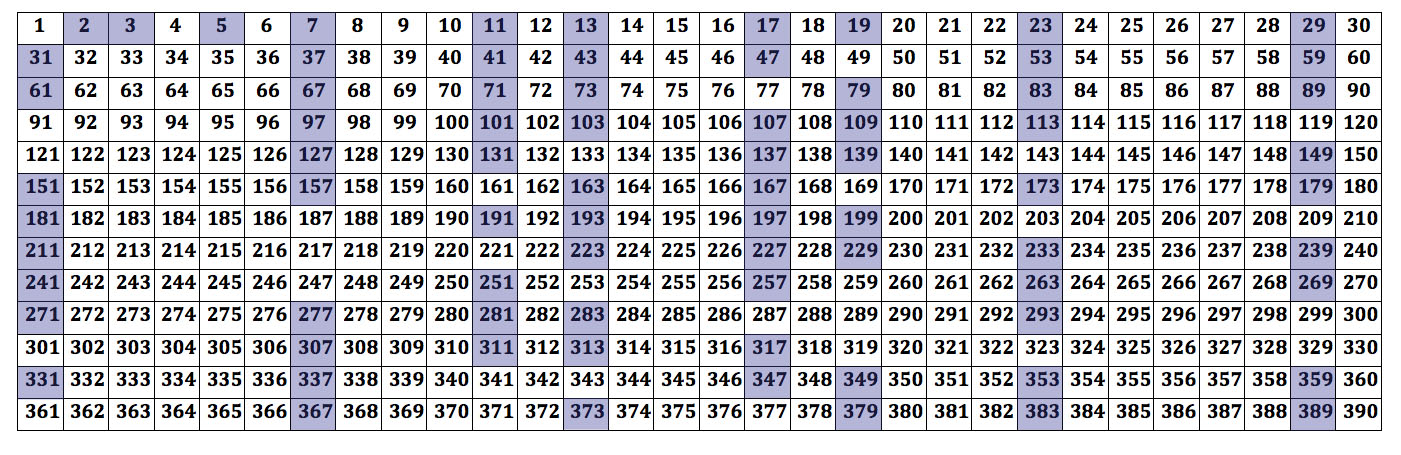
\includegraphics[scale=0.3]{figures/Numberrectangle-with-colored-primes_Irisprime.jpg}
\caption[Primzahlen unter den ersten 390 natürlichen Zahlen -- farblich markiert]
        {Primzahlen unter den ersten 390 natürlichen Zahlen -- farblich markiert\protect\footnotemark}
\label{Primes-in-a-390-integer-rechtangle-figure}
\end{center}
\end{figure}
\footnotetext{%
   Grafik von
   \url{http://mathforum.org/mathimages/index.php/Image:Irisprime.jpg}, 30*13-Rechteck
   % BE_8.8.2018: mathforum.org seemed to become https://www.nctm.org/mathforum/,
   %              but we couldn't find this image again.
}

\begin{figure}[!hb]
\begin{center}
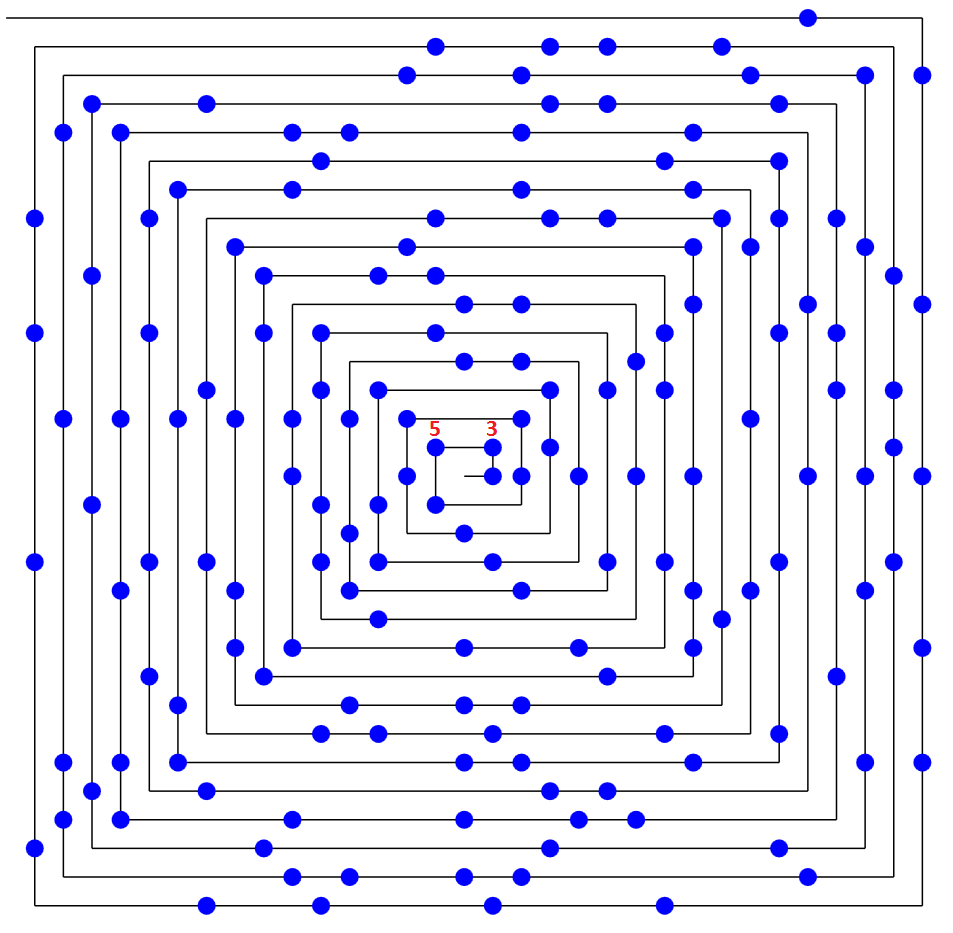
\includegraphics[scale=0.41]{figures/Ulam_spiral_via-CT2-within-1-999.png}
\caption[Primzahlen unter den ersten 999 natürlichen Zahlen -- als Ulam-Spirale]
        {Primzahlen unter den ersten 999 natürlichen Zahlen -- als Ulam-Spirale\protect\footnotemark}
\label{Primes-in-a-999-integer-ulam-spiral-figure}
\end{center}
\end{figure}
\footnotetext{%
   Grafik von CT2, Menü Kryptotutorien, Die Welt der Primzahlen,
   Verteilung der Primzahlen, Ulam-Spirale; 32*32 Punkte.\index{CT2}
}
%\newpage
\begin{figure}[!hb]
\begin{center}
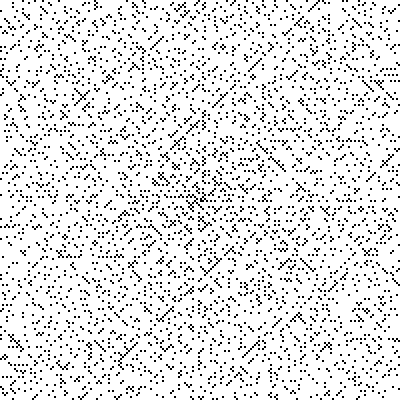
\includegraphics{figures/Ulam_spiral_Wikipedia.png}
\caption[Primzahlen unter den ersten 4000 natürlichen Zahlen -- als Ulam-Spirale]
        {Primzahlen unter den ersten 4000 natürlichen Zahlen -- als Ulam-Spirale\protect\footnotemark}
\label{Primes-in-a-4000-integer-ulam-spiral-figure}
\end{center}
\end{figure}
\footnotetext{%
   Grafik von
   \url{http://mathforum.org/mathimages/index.php/Image:Ulam_spiral.png}, 200*200 Ulam-Spirale
   % BE_8.8.2018: mathforum.org seemed to become https://www.nctm.org/mathforum/,
   %              but we couldn't find this image again.
   }



\newpage
\begin{satz}\label{thm-pz-sqr}
Jede ganze Zahl $m$ größer als $1$ besitzt einen kleinsten Teiler größer als $1$.
Dieser ist eine Primzahl $p$. Sofern $m$ nicht selbst eine Primzahl ist, gilt:
$p$ ist kleiner oder gleich der Quadratwurzel aus $m$.
\end{satz}

Aus den Primzahlen lassen sich alle ganzen Zahlen größer als $1$ zusammensetzen --- und das sogar in
einer eindeutigen Weise. Dies besagt der \textbf{1. Hauptsatz der Zahlentheorie} (= Hauptsatz der elementaren Zahlentheorie =
fundamental theorem of arithmetic = fundamental building block of all positive integers).\index{Zahlentheorie!Hauptsatz}

\begin{satz}\label{thm-pz-prod}
Jedes Element $n$ größer als $1$ der natürlichen Zahlen lässt sich als Produkt
$n = p_1 \cdot p_2 \cdot \dots \cdot p_m$ von Primzahlen schreiben.
Sind zwei solche Zerlegungen
$$n =  p_1 \cdot p_2 \cdots p_m = p'_1 \cdot p'_2 \cdots p'_{m'}$$
gegeben, dann gilt nach eventuellem Umsortieren $\;m = m'\;$ und  für alle $i$:  $\;p_i = p'_i$. \\
($p_1, p_2, \dots, p_m$ nennt man die Primfaktoren\index{Primfaktor} von n).
\end{satz}

In anderen Worten: Jede natürliche Zahl außer der $1$ lässt sich auf genau eine Weise als Produkt von
Primzahlen schreiben, wenn man von der Reihenfolge der Faktoren absieht. Die Faktoren sind also
eindeutig (die {\em Expansion in Faktoren} ist eindeutig)!
Zum Beispiel ist
$$ 60 = 2 \cdot 2 \cdot 3 \cdot 5 = 2^2\cdot 3^1 \cdot 5^1 $$
Und das ist --- bis auf eine veränderte Reihenfolge der Faktoren
--- die einzige Möglichkeit, die Zahl $60$ in Primfaktoren zu
zerlegen. Wenn man nicht nur Primzahlen als Faktoren zulässt,
gibt es mehrere Möglichkeiten der Zerlegung in Faktoren und die
\textbf{Eindeutigkeit} (\hypertarget{uniqueness}{uniqueness}) geht verloren:
$$ 60 = 1 \cdot 60 = 2 \cdot 30 = 4 \cdot 15 = 5 \cdot 12 =6 \cdot 10 = 2 \cdot 3 \cdot 10 =
        2 \cdot 5 \cdot 6 = 3 \cdot 4 \cdot 5 = \cdots . $$

Der folgende Absatz wendet sich eher an die mit der mathematischen Logik vertrauteren Menschen:
Der 1. Hauptsatz ist nur scheinbar selbstverständlich\label{remFundTheoOfArithm}. Man kann viele andere Zahlenmengen
(ungleich der positiven ganzen Zahlen größer als 1) konstruieren, bei denen selbst eine Zerlegung in
die Primfaktoren dieser Mengen nicht eindeutig ist:
In der Menge $M = \{1, 5, 10, 15, 20, \cdots\}$ gibt es unter der Multiplikation kein Analogon zum Hauptsatz.
Die ersten fünf Primzahlen dieser Folge sind $5, 10, 15, 20, 30$ (beachte: $10$ ist prim, da innerhalb
dieser Menge $5$ kein Teiler von $10$ ist --- das Ergebnis $2$ ist kein Element der gegebenen Grundmenge
$M$). Da in $M$ gilt:
$$ 100 = 5 \cdot 20 = 10 \cdot 10 $$
und sowohl $5, 10, 20$ Primzahlen dieser Menge sind, ist hier die Zerlegung in Primfaktoren nicht
eindeutig.

% --------------------------------------------------------------------------
\section{Wie viele Primzahlen gibt es?}
\label{Section_pr_How-many-primes}

Für die natürlichen Zahlen sind die Primzahlen vergleichbar mit den
Elementen in der Chemie oder den Elementarteilchen in der Physik
(vgl. \cite[S. 22]{Blum1999}).

Während es nur $92$ natürliche chemische Elemente gibt, ist die Anzahl
der Primzahlen unbegrenzt.
Das wusste schon der Grieche \index{Euklid} Euklid\footnote{%
Euklid, griechischer Mathematiker des 4./3. Jahrhunderts vor Christus.
Wirkte an der Akademie in Alexandria und verfasste mit den
\glqq Elementen\grqq~ das bekannteste systematische Lehrbuch
der griechischen Mathematik.}
im dritten vorchristlichen Jahrhundert.

\begin{satz}[Euklid\footnote{Die üblich gewordene Benennung bedeutet nicht
unbedingt, dass Euklid der Entdecker des Satzes ist, da dieser
nicht bekannt ist. Der Satz wird bereits in Euklids \glqq Elementen\grqq~(Buch IX, Satz 20)
formuliert und bewiesen. Die dortige Formulierung ist insofern bemerkenswert,
als sie das Wort \glqq unendlich\grqq~ nicht verwendet; sie lautet
$$
O\acute{\iota}~\pi\varrho\tilde{\omega}\tau o \iota~\grave{\alpha}\varrho\iota\vartheta\mu o\grave{\iota}~
\pi\lambda\varepsilon\acute{\iota}o \upsilon\varsigma~\varepsilon\grave{\iota}\sigma\grave{\iota}~
\pi\alpha\nu\tau\grave{o}\varsigma~\tau o \tilde{\upsilon}~
\pi\varrho o \tau\varepsilon\vartheta\acute{\varepsilon}\nu\tau o \varsigma~
\pi\lambda\acute{\eta}\vartheta\ o \upsilon\varsigma~
\pi\varrho\acute{\omega}\tau\omega\nu~
\grave{\alpha}\varrho\iota\vartheta\mu\tilde{\omega}\nu,
$$
zu deutsch: Die Primzahlen sind mehr als jede vorgegebene Menge von Primzahlen.
}]\label{thm-pz-euklid}\hypertarget{thm-pz-euklid}{} % Ende der Fußnote
Die Folge der Primzahlen bricht nicht ab, es gibt also unendlich
viele Primzahlen.
\end{satz}

Sein Beweis, dass es unendlich viele Primzahlen gibt, gilt bis heute als
ein Glanzstück mathematischer Überlegung und Schlussfolgerung
(\textbf{Widerspruchsbeweis}\index{Widerspruchsbeweis}).
Er nahm an, es gebe nur endlich viele Primzahlen und damit eine größte
Primzahl. Daraus zog er solange logische Schlüsse, bis er auf einen
offensichtlichen Widerspruch stieß. Damit musste etwas falsch sein. Da
sich in die Schlusskette kein Lapsus eingeschlichen hatte, konnte es nur
die Annahme sein. Demnach musste es unendlich viele Primzahlen geben!\\

\hypertarget{ht_euclid}{}
\index{Euklids Widerspruchsbeweis}\index{Widerspruchsbeweis}
% \paragraph*{Euklids Widerspruchsbeweis}
% Bei /paragraph den * angefügt, damit es auch bei 4 Ebenen nicht im Inh.verzeichnis erscheint
% führt die Argumentation wie folgt:
\begin{Beweis}{nach Euklid (Widerspruchsbeweis)\\}
\textbf{Annahme:} \quad Es gibt {\em endlich} viele Primzahlen.
\\*[4pt] \textbf{Schluss:} \quad Dann lassen sie sich auflisten $p_1
< p_2 < p_3 < \dots < p_n$, wobei $n$ für die (endliche) Anzahl
der Primzahlen steht. $p_n$ wäre also die größte Primzahl. Nun
betrachtet Euklid die Zahl $a = p_1 \cdot p_2 \cdots p_n +1$.
Diese Zahl kann keine Primzahl sein, da sie in unserer
Primzahlenliste nicht auftaucht. Also muss sie durch eine Primzahl
teilbar sein. D.h. es gibt eine natürliche Zahl $i$ zwischen $1$
und $n$, so dass $p_i$ die Zahl $a$ teilt. Natürlich teilt $p_i$
auch das Produkt $a-1 = p_1 \cdot p_2 \cdots p_n$, da $p_i$ ja ein
Faktor von $a-1$ ist. Da $ p_i $ die Zahlen $ a $ und $ a-1 $
teilt, teilt sie auch die Differenz dieser Zahlen. Daraus folgt:
$p_i$ teilt  $a - (a-1) = 1$. $p_i$ müsste also $1$ teilen und
das ist unmöglich.\\*[4pt]
\textbf{Widerspruch}: \quad Unsere Annahme war falsch.\par

Also gibt es {\em unendlich} viele Primzahlen
(siehe \hyperlink{primhfk}{Übersicht unter \ref{s:primhfk}} über die
Anzahl von Primzahlen in verschiedenen Intervallen).
\end{Beweis}

\par \vskip + 10pt

Wir erwähnen hier auch noch eine andere, auf den ersten Blick
überraschende Tatsache, dass nämlich in der Folge aller
Primzahlen $p_1, p_2, \cdots $ Lücken von beliebig großer
Länge $n$ auftreten. Unter den $n$ aufeinanderfolgenden
natürlichen Zahlen
$$
    (n+1)!+2, \cdots, (n+1)!+(n+1),
$$
ist keine eine Primzahl, da ja in ihnen der Reihe nach die
Zahlen $2,\cdots, n+1$ als echte Teiler enthalten sind
(Dabei bedeutet $n!$ das Produkt der ersten $n$ natürlichen
Zahlen, also $n!=n*(n-1)* \cdots *3*2*1$).


% --------------------------------------------------------------------------
% --------------------------------------------------------------------------
%% \vskip + 20pt
\newpage
\section{Die Suche nach sehr großen Primzahlen}
\label{search_for_very_big_primes}   % chap. 3.4

Die größten heute bekannten Primzahlen haben mehrere
Millionen Stellen.\footnote{%
	In CT1\index{CT1} können Sie über das Menü
	\textbf{Einzelverfahren \textbackslash{} Zahlentheorie
	interaktiv \textbackslash{} Mersenne-Zahlen berechnen}
	alle Stellen einer solch großen Zahl sehr schnell berechnen.
	%% zur Die 50. – und bislang größte bekannte – Mersenne-Primzahl
	%% Auf meinem PC war die Zahl in 20 sec berechnet (wohlgemerkt, das ist nur die Zeit für die Berechnung der Zweierpotenz, nicht der Beweis, dass die Zahl prim ist). Das Abspeichern und Anzeigen der knapp 23 MB großen Zahl dauerte dann länger als die Berechnung.
}
Das ist unvorstellbar groß. Die Anzahl der Elementarteilchen im
Universum wird auf eine \glqq nur\grqq\ $80$-stellige Dezimalzahl
geschätzt \hyperlink{grosord}{(siehe Übersicht unter \ref{s:grosord}
über verschiedene Größenordnungen / Dimensionen)}.



% --------------------------------------------------------------------------
\hypertarget{RecordPrimes}{}
\subsection{Die 30+ größten bekannten Primzahlen (Stand Jan. 2018)}  % Eyecatcher_neue-Mersenne
\index{Primzahlrekorde}
\label{RecordPrimes}

In der folgenden Tabelle \ref{L_n_Largest_Known-Primes} sind die größten, derzeit bekannten Primzahlen und
eine Beschreibung des jeweiligen Zahlentyps aufgeführt.\footnote{%
Eine jeweils aktuelle Fassung findet sich im Internet
unter  \url{https://primes.utm.edu/primes/search.php?Number=1000},
% at   \url{http://primes.utm.edu/largest.html},
unter  \url{http://primes.utm.edu/mersenne/index.html}, und
unter  \url{http://www.mersenne.org/primes/}.
}
% Bsp-Meldungen
% - http://www.heise.de/newsticker/meldung/Neue-groesste-bekannte-Primzahl-mit-ueber-22-Millionen-Stellen-gefunden-3079127.html  20.01.2016
% - http://www.spiegel.de/wissenschaft/mensch/primzahlen-neue-rekord-zahl-mit-22-33-millionen-stellen-gefunden-a-1072883.html  20.1.16
%
%	10 & $1.372.930^{131.072}+1$ &   804.474 & 2003 & Verallg. Fermat\footnote{%
% $ 1.372.930^{131.072} + 1 = 1.372.930^{(2^{17})}+1 $ } \\

\index{Mersenne!Mersennezahl!verallgemeinert}
\index{Fermat!Fermatzahl!verallgemeinert}

%% Der Aufruf von \rowno[0] machte immer auch gleich eine Ausgabe.
%% Ich wollte Ausgabe unterdrücken (suppress, discard-command-output)
%% \setcounter{rowno}{0} tat nicht, weil rowno ein command (e ex. nur interner counter)
\ignoreoutput{\rowno[0]} % Could have used \rowno[1] in the 1st row of the table.
                         % However, to make maintenance for adding new records
			 % easier, I wanted to have always "\rowno" in each line.
                         % Therefore I have to call the command (which sets the
			 % counter and increases it by one) before, but suppress
			 % the output.

\begin{table}[ht]   % Vgl. http://primes.utm.edu/largest.html
\begin{center}
\begin{tabular}{|c|cccc|}
\hline \rule{0pt}{10pt}     % Eyecatcher_neue-Mersenne
 	& \textbf{Definition} & \textbf{Dezimalstellen} & \textbf{Wann} & \textbf{Beschreibung} \\
\hline \rule{0pt}{15pt} % Damit erreicht, dass die Exponenten nicht in die waagrechte Linie hineinragen.
        \rowno & $2^{77.232.917}-1$ & 23.249.425 & 2018 & Mersenne, 50. bekannte \\
        \rowno & $2^{74.207.281}-1$ & 22.338.618 & 2016 & Mersenne, 49. bekannte \\
	\rowno & $2^{57.885.161}-1$ & 17.425.170 & 2013 & Mersenne, 48. bekannte \\
	\rowno & $2^{43.112.609}-1$ & 12.978.189 & 2008 & Mersenne, M-47 \\
	\rowno & $2^{42.643.801}-1$ & 12.837.064 & 2009 & Mersenne, M-46 \\
	\rowno & $2^{37.156.667}-1$ & 11.185.272 & 2008 & Mersenne, M-45 \\
	\rowno & $2^{32.582.657}-1$ &  9.808.358 & 2006 & Mersenne, M-44 \\
	\rowno & $2^{30.402.457}-1$ &  9.152.052 & 2005 & Mersenne, M-43 \\
	\rowno & $2^{25.964.951}-1$ &  7.816.230 & 2005 & Mersenne, M-42 \\
	\rowno & $2^{24.036.583}-1$ &  7.235.733 & 2004 & Mersenne, M-41 \\
	\rowno & $2^{20.996.011}-1$ &  6.320.430 & 2003 & Mersenne, M-40 \\
	\rowno & $2^{13.466.917}-1$ &  4.053.946 & 2001 & Mersenne, M-39 \\
	\rowno & $19.249 \cdot 2^{13.018.586}+1$ & 3.918.990 & 2007 & Verallgem. Mersenne\footnotemark \\%%%

	\rowno & $3 \cdot 2^{11.895.718}-1$ & 3.580.969 & 2015 & Verallgem. Mersenne \\
	\rowno & $3 \cdot 2^{11.731.850}-1$ & 3.531.640 & 2015 & Verallgem. Mersenne \\
	\rowno & $3 \cdot 2^{11.484.018}-1$ & 3.457.035 & 2014 & Verallgem. Mersenne \\
	\rowno & $3 \cdot 2^{10.829.346}+1$ & 3.259.959 & 2014 & Verallgem. Mersenne \\
	\rowno & $ 475.856^{524.288}+1$ &   2.976.633 & 2012 & Verallgem. Fermat \\
	\rowno & $ 356.926^{524.288}+1$ &   2.911.151 & 2012 & Verallgem. Fermat \\
	\rowno & $ 341.112^{524.288}+1$ &   2.900.832 & 2012 & Verallgem. Fermat \\

	\rowno & $27.653 \cdot 2^{9.167.433}+1$ & 2.759.677 & 2005 & Verallgem. Mersenne \\%%%

	\rowno & $90.527 \cdot 2^{9.162.167}+1$ & 2.758.093 & 2010 & Verallgem. Mersenne \\
	\rowno & $2.038 \cdot 366^{1.028.507}-1$ & 2.636.562 & 2016 & Verallgem. Fermat \\
	\rowno & $75.898^{524.288}+1$ & 2.558.647 & 2011 & Verallgem. Fermat \\

	\rowno & $28.433 \cdot 2^{7.830.457}+1$ & 2.357.207 & 2004 & Verallgem. Mersenne \\%%%

	\rowno & $502.573 \cdot 2^{7.181.987}-1$ & 2.162.000 & 2014 & Verallgem. Mersenne \\
	\rowno & $402.539 \cdot 2^{7.173.024}-1$ & 2.159.301 & 2014 & Verallgem. Mersenne \\
	\rowno & $161.041 \cdot 2^{7.107.964}+1$ & 2.139.716 & 2015 & Verallgem. Mersenne \\
	\rowno & $3 \cdot 2^{7.033.641}+1$ & 2.117.338 & 2011 & Verallgem. Mersenne \\
	\rowno & $33.661 \cdot 2^{7.031.232}+1$ & 2.116.617 & 2007 & Verallgem. Mersenne \\

	\rowno & $2^{ 6.972.593}-1$ & 2.098.960 & 1999 & Mersenne, M-38 \\%%%
        ... &  &  &  & \\
%	16 & $5.359 \cdot 2^{5.054.502}+1$ & 1.521.561 & 2003 & Verallgem. Mersenne \\
%	17 & $4.847 \cdot 2^{3.321.063}+1$ & 999.744 & 2005 & Verallgem. Mersenne \\
%	18 & $3 \cdot 2^{3.136.255}-1$ & 944.108 & 2007 & Verallgem. Mersenne \\
%	19 & $2^{ 3.021.377}-1$ &   909.526 & 1998 & Mersenne, M-37 \\
%	20 & $2^{ 2.976.221}-1$ &   895.932 & 1997 & Mersenne, M-36 \\
%	21 & $222.361 \cdot 2^{2.854.840}+1$ & 859.398 & 2006 & Verallgem. Mersenne \\
        % Eyecatcher_neue-Mersenne
	329 & $1.372.930^{131.072}+1$ &   804.474 & 2003 & Verallgem. Fermat\footnotemark \\
%	23 & $1.361.244^{131.072}+1$ &   803.988 & 2004 & Verallgem. Fermat \\
%	24 & $1.176.694^{131.072}+1$ &   795.695 & 2003 & Verallgem. Fermat \\
        ... &  &  &  & \\
        % Eyecatcher_neue-Mersenne
	343 & $342.673 \cdot 2^{2.639.439}-1$ & 794.556 & 2007 & Verallgem. Mersenne \\

   \hline
\end{tabular}
\caption{Die 30+ größten Primzahlen und ihr jeweiliger Zahlentyp
         (Stand Apr. 2018)}    %  Eyecatcher_neue-Mersenne
\label{L_n_Largest_Known-Primes}
\end{center}
\end{table}
\addtocounter{footnote}{-1}
\footnotetext{\index{Zahlen!Sierpinski}\index{Seventeen or Bust SoB}%
Diese Zahl wurde am 26.3.2007 im verteilt rechnenden Internet-Projekt
"`Seventeen or Bust"' (SoB) (\url{https://de.wikipedia.org/wiki/Seventeen_or_Bust})
% (\url{http://www.seventeenorbust.com}) Not accessible at July 19, 2016
gefunden. Anders als das bekannte \hyperlink{GIMPS-project}{GIMPS-Projekt}
(Kapitel~\ref{zahlentyp_mersenne}), das immer größere der unendlich
vielen Primzahlen aufspürt, könnte SoB aber irgendwann mal die
gesetzte Aufgabe vollständig erledigt haben.

Das SoB-Projekt versucht rechnerisch zu beweisen, dass die Zahl
$k = 78.557$ die kleinste Sierpinski-Zahl ist (John Selfridge
bewies 1962, dass $78.557$ eine Sierpinski-Zahl ist).

Der berühmte polnische Mathematiker Waclaw Sierpinski (1882 bis 1969) hatte im
Jahre 1960 nachgewiesen, dass es unendlich viele ungerade natürliche Zahlen k gibt,
die folgende Eigenschaft erfüllen: Für jede Sierpinski-Zahl k gilt: Sämtliche Zahlen
$N = k \cdot 2^{n}+1$ sind für alle natürlichen $n>=1$ zusammengesetzte Zahlen
(Sierpinski's Composite Number Theorem,
\url{http://mathworld.wolfram.com/SierpinskisCompositeNumberTheorem.html}).

Am Projektanfang im Jahre 2002 gab es noch 17 mögliche Kandidaten $< 78557$ (daher der Name des Projekts "`Seventeen or Bust"'). Es reicht, wenn man ein einziges Gegenbeispiel findet, um einen Kandidaten k auszuschließen, also ein einziges $n>=1$ zu finden, so dass $N = k \cdot 2^{n}+1$ prim ist. Dass bei dieser Suche sehr große Primzahlen gefunden werden, ist also eigentlich nur ein "`Nebenprodukt"' der Aufgabenstellung.

Vergleiche auch die Meldung vom 10.05.2007: %%% Diesen Link nur in der deutschen Fassung.
\url{http://www.heise.de/newsticker/meldung/89582}.
%% http://www.heise.de/newsticker/meldung/Neue-groesste-bekannte-Nicht-Mersenne-Primzahl-177280.html

Seit Mitte April 2016 ist der SoB-Server nicht mehr erreichbar und damit die Zukunft des Grundprojektes ungewiss.
}
\addtocounter{footnote}{1}
\footnotetext{%
Verallgemeinerte Fermatzahl: $ 1.372.930^{131.072} + 1 = 1.372.930^{(2^{17})}+1 $
\index{Fermat!Fermatzahl!verallgemeinert}
}
%be_2005: footnotemark und footnotetext statt nur footnote (sonst sieht man nur
%         die Fussnoten-Nr., aber nicht den Text!

\clearpage  %% Erzwingen, dass die Tabelle noch in diesem Kapitel und vor Fig. 3.4




Die zeitliche Entwicklung wird in Abbildung \ref{Figure_Caldwell_Largest-Known-Prime-From1975}
verdeutlicht. Sie startet mit M21701 (gefunden 1978). Bitte die logarithmische vertikale Skala beachten.
\begin{figure}[ht]
\begin{center}
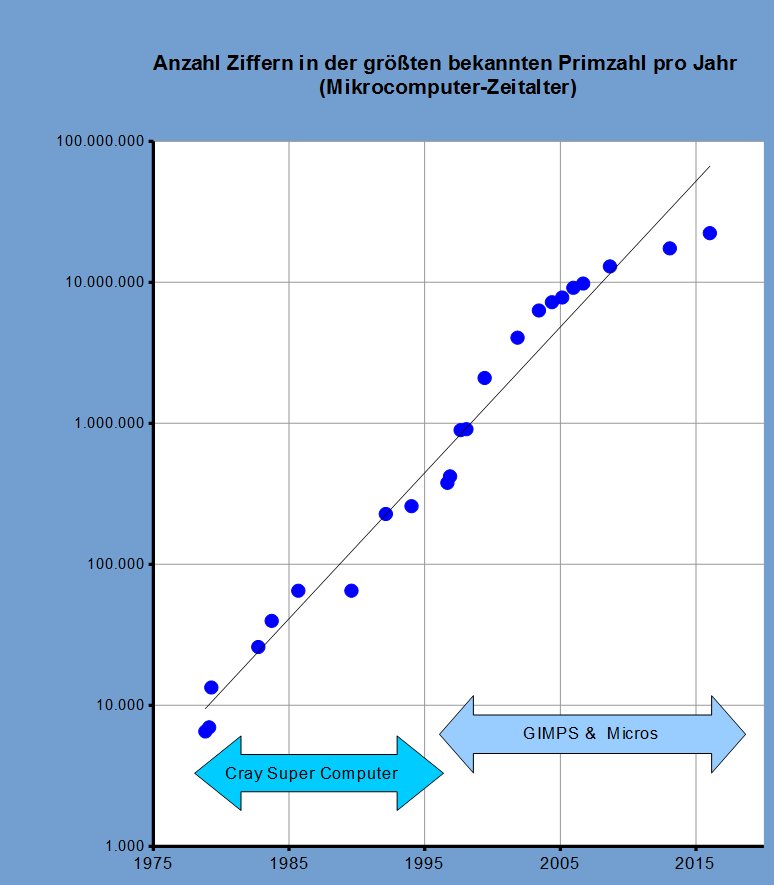
\includegraphics[scale=0.7]{figures/Caldwell_From1975-2016-de.png}
\caption[Anzahl Ziffern der größten bekannten Primzahl nach Jahren seit 1975]
        {Anzahl Ziffern der größten bekannten Primzahl nach Jahren (Stand Juli 2016)\footnotemark}
\label{Figure_Caldwell_Largest-Known-Prime-From1975}
\end{center}
\end{figure}
\index{Caldwell, Chris}
\footnotetext{
  Quelle: Chris Caldwell, \url{http://primes.utm.edu/notes/by_year.html}
}

Die größte, momentan bekannte Primzahl ist eine Mersenne-Primzahl.
Diese wurde vom \hyperlink{GIMPS-project}{GIMPS-Projekt}
(Kapitel~\ref{zahlentyp_mersenne}) gefunden.
Unter den größten bekannten Primzahlen befinden sich außerdem Zahlen
vom Typ \hyperlink{generalizedMersennenumbers}{verallgemeinerte Mersennezahl}
(Kapitel~\ref{generalized-mersenne-no1})
und
vom Typ \hyperlink{generalizedFermatprimes}{verallgemeinerte Fermatzahl}
(Kapitel~\ref{generalized-fermat}).

% clearpage war nötig, denn sonst stand Tab. 3.1 erst auf S. 90 unter 3.8.1
% Im Englischen passt das -- ohne händische Korrektur -- alles noch in 3.4.1.
\clearpage


% --------------------------------------------------------------------------
\hypertarget{MersenneNumbers01}{}
\subsection{Mersennezahlen und Mersenne-Primzahlen}
\label{zahlentyp_mersenne}
\index{Mersenne!Mersennezahl}

Nahezu alle bekannten riesig großen Primzahlen sind spezielle
Kandidaten, sogenannte {\em Mersennezahlen}\footnote{%
Marin Mersenne, französischer Priester und Mathematiker,
08.09.1588$-$01.09.1648.
\index{Mersenne, Marin}
}
der Form $2^p -1,$ wobei $p$ eine Primzahl ist.
Nicht alle Mersennezahlen sind prim:
$$
\begin{array}{cl}
2^2 - 1 = 3 & \Rightarrow {\rm prim} \\
2^3 - 1 = 7 & \Rightarrow {\rm prim} \\
2^5 - 1 = 31    & \Rightarrow {\rm prim} \\
2^7 - 1 = 127    & \Rightarrow {\rm prim} \\
2^{11} - 1 = 2.047 = 23 \cdot 89    & \Rightarrow  {\rm NICHT~prim} !
\end{array}
$$

\index{Zahlen!Mersennezahl}
\index{Mersenne!Mersennezahl}
\index{Mersenne!Satz}

Dass Mersennezahlen nicht immer Primzahlen (Mersenne-Primzahlen) sind,
wusste auch schon Mersenne (siehe Exponent $p = 11$).
Eine Mersennezahl, die prim ist, wird Mersenne-Primzahl
\index{Mersenne!Mersenne-Primzahl} genannt.  \\

Dennoch ist ihm der interessante Zusammenhang zu verdanken, dass eine
Zahl der Form $2^n-1$ keine Primzahl sein kann, wenn $n$ eine
zusammengesetzte Zahl ist:

\begin{satz}[Mersenne]\label{thm-pz-mersenne}
  Wenn $2^n - 1$ eine Primzahl ist, dann folgt, $n$ ist ebenfalls eine
  Primzahl (oder anders formuliert: $2^n - 1$ ist nur dann prim,
  wenn $n$ prim ist).
\end{satz}

\begin{Beweis}{}
Der Beweis des Satzes von Mersenne kann durch Widerspruch
\index{Widerspruchsbeweis}
durchgeführt werden. Wir nehmen also an, dass es eine
zusammengesetzte natürliche Zahl $ n $ mit echter Zerlegung
$\; n=n_1 \cdot n_2 $
gibt, mit der Eigenschaft, dass $ 2^n -1 $ eine
Primzahl ist.

Wegen
\begin{eqnarray*}
(x^r-1)((x^r)^{s-1} + (x^r)^{s-2} + \cdots + x^r +1) & = &  ((x^r)^s + (x^r)^{s-1} + (x^r)^{s-2} + \cdots + x^r) \\
&  & -((x^r)^{s-1} + (x^r)^{s-2} + \cdots + x^r +1)  \\
& = & (x^r)^s -1 = x^{rs } -1,
\end{eqnarray*}
folgt
\[ 2^{n_1 n_2} - 1 = (2^{n_1} -1)((2^{n_1})^{n_2 -1} + (2^{n_1})^{n_2 -2} + \cdots + 2^{n_1} + 1). \]
Da $ 2^n - 1 $ eine Primzahl ist, muss einer der obigen beiden
Faktoren auf der rechte Seite gleich 1 sein. Dies kann nur dann
der Fall sein, wenn $ n_1 =1 $ oder $ n_2 =1$ ist. Dies ist aber
ein Widerspruch zu unserer Annahme. Deshalb ist unsere Annahme
falsch. Also gibt es keine zusammengesetzte Zahl $ n, $ so dass $
2^n -1 $ eine Primzahl ist.
\end{Beweis}

\vskip + 5pt
\hypertarget{Mer-nums-not-always-prim}{}
Leider gilt dieser Satz nur in einer Richtung (die Umkehrung gilt
nicht, keine Äquivalenz): Das heißt, dass es prime Exponenten gibt,
für die die zugehörige Mersennezahl \textbf{nicht} prim ist (siehe das
obige Beispiel $2^{11}-1, $ wo $11$ prim ist, aber $2^{11}-1$ nicht).
% Das ist auf dem Cover = Titelblatt.

Mersenne behauptete, dass $2^{67}-1$ eine Primzahl ist. Auch zu
dieser Behauptung gibt es eine interessante mathematische Historie:
Zuerst dauerte es über 200 Jahre, bis \index{Lucas, Edouard}
Edouard Lucas (1842-1891) bewies, dass diese Zahl zusammengesetzt
ist. Er argumentierte aber indirekt und kannte keinen der
Faktoren. 1903 zeigte Cole\index{Cole, Frank Nelson}\footnote{%
Frank Nelson Cole, amerikanischer Mathematiker, 20.09.1861$-$26.05.1926.\\
},
aus welchen Faktoren diese Primzahl besteht:
$$ 2^{67} -1
=147. 573. 952. 589. 676. 412. 927 = 193. 707. 721 \cdot 761. 838. 257. 287. $$
Er gestand, 20 Jahre an der \textbf{Faktorisierung} \index{Faktorisierung}
(Zerlegung in ein Produkt aus Primfaktoren)%
\footnote{%
  Mit CT1\index{CT1} können Sie Zahlen auf folgende Weise
  faktorisieren: Menü \textbf{Einzelverfahren \textbackslash{} RSA-Kryptosystem
  \textbackslash{} Faktorisieren einer Zahl}. \\
  In sinnvoller Zeit zerlegt CT1 mit dem Quadratischen Sieb (QS)
  auf einem Einzel-PC Zahlen bis 250 Bit Länge. Zahlen größer
  als 1024 Bit werden zur Zeit von CT1 sowieso nicht angenommen.\\

   CT2\index{CT2} hat die Komponente GeneralFactorizer
  (basierend auf YAFU\index{YAFU}). Diese ist schneller als die in CT1
  implementierten Funktionen.
  Damit bietet CT2 die folgenden Faktorisierungsverfahren:
  \begin{compactitem}
   \item[-] Brute-force mit kleinen Primzahlen
   \item[-] Fermat
   \item[-] Shanks Square Forms Factorization (squfof)
   \item[-] Pollard rho
   \item[-] Pollard p-1
   \item[-] Williams p+1
   \item[-] Lenstra Elliptic Curve Method (ECM)
   \item[-] Self-initializing Quadratic Sieve (SIQS)
   \item[-] Multiple-polynomial Quadratic Qieve (MPQS)
   \item[-] Special Number Field Sieve (SNFS)
   \item[-] General Number Field Sieve (GNFS).
  \end{compactitem}

   CT2 hat begonnen, mit einer allgemeinen Infrastruktur für verteiltes
  Rechnen zu experimentieren (CrypCloud\index{CrypCloud}, die sowohl Peer-to-Peer
  als auch zentralisiert eingesetzt werden kann). Damit wird CT2 in Zukunft in die
  Lage versetzt, Berechnungen auf viele Computer zu verteilen.
  Was man erreichen kann, wenn die Komponenten für die Parallelisierung eingerichtet
  sind, zeigte ein Cluster zur verteilten Kryptoanalyse von DES und AES:
  Stand 21. März 2016 funktionierte ein Brute-force-Angriff (verteilte Schlüsselsuche)
  gegen AES auf 50 i5-PCs, jeder mit 4 virtuelles CPU-Kernen. Diese 200 virtuellen
  \glqq Worker Threads\grqq~konnten ca. 350 Millionen AES-Schlüssel/sec testen. Die
  \glqq Cloud\grqq~verarbeitete dabei insgesamt ca. 20 GB/sec an Daten. CrypCloud
  ist eine Volunteering-Cloud, so dass CT2-Nutzer sich freiwillig bei
  verteilten Jobs anschließen können.

   Die aktuellen Faktorisierungsrekorde finden Sie in Kapitel
  \ref{nt:NoteFactorization}.
  \index{Faktorisierung!Faktorisierungsrekorde}
}
dieser 21-stelligen Dezimalzahl gearbeitet zu haben!

Dadurch, dass man bei den Exponenten der Mersennezahlen nicht alle
natürlichen Zahlen verwendet, sondern nur die Primzahlen, engt man
den {\em Versuchsraum} deutlich ein. Die derzeit bekannten $50$
    % Eyecatcher_neue-Mersenne  % be_2005_UPDATEN_if-new-mersenne-prime-appears
Mersenne-Primzahlen\index{Primzahl!Mersenne}\index{Mersenne!Mersenne-Primzahl}
gibt es für die folgenden Exponenten\footnote{%
  Landon Curt Noll\index{Noll, Landon Curt} listet in einer Tabelle alle
  bekannten Mersenne-Primzahlen samt Entdeckungsdatum und Wert in Zahlen-
  und Wortform auf:
      \url{http://www.isthe.com/chongo/tech/math/prime/mersenne.html}\\
  Siehe auch:
      \url{http://www.utm.edu/}.
}
$$
\begin{array}{c}
2, ~ 3, ~ 5, ~ 7, ~ 13, ~ 17, ~ 19, ~ 31, ~ 61, ~ 89, ~ 107, ~ 127, ~ 521, ~ 607, ~ 1.279, ~ 2.203, ~ 2.281, ~ 3.217, ~ 4.253, \\
4.423, ~9.689, ~ 9.941, ~ 11.213, ~ 19.937, ~ 21.701, ~ 23.207, ~ 44.497, ~ 86.243, ~ 110.503, ~ 132.049,\\
216.091, ~ 756.839, ~ 859.433, ~ 1.257.787, ~ 1.398.269, ~ 2.976.221, ~ 3.021.377, ~ 6.972.593,\\
 ~ 13.466.917, ~ 20.996.011, ~ 24.036.583, ~ 25.964.951, ~ 30.402.457, ~ 32.582.657,\\
 ~ 37.156.667, ~ 42.643.801, ~ 43.112.609, ~ 57.885.161, ~ 74.207.281, ~ 77.232.917.
% be_2005_UPDATEN_if-new-mersenne-prime-appears          ~ xxx.xxx.xxx.
\end{array}
$$


\vskip +10 pt
Die $19$. Zahl mit dem Exponenten $4.253$ war die erste mit mindestens $1.000$
Stellen im Zehnersystem (der Mathematiker Samual \index{Yates,
Samual} Yates prägte dafür den Ausdruck {\em titanische}
\index{Primzahl!titanisch} Primzahl; sie wurde 1961 von Hurwitz
gefunden); die $27$. Zahl mit dem Exponenten $44.497$ war die
erste mit mindestens $10.000$ Stellen im Zehnersystem (Yates
prägte dafür den Ausdruck \index{Primzahl!gigantisch}  {\em
gigantische} Primzahl. Diese Bezeichnungen sind heute längst
veraltet).

% \vskip - 4pt 
% \begin{quote}
% (Der Supercomputerhersteller SGI Cray Research beschäftigte nicht
% nur hervorragende Mathematiker, sondern benutzte die Primzahltests
% auch als Benchmarks für seine Maschinen.)
% \end{quote}

% \vspace{-10pt}
% \begin{itemize}
%  \item[] \url{http://reality.sgi.com/chongo/prime/prime_press.html}
% \end{itemize}


\vskip +10 pt
Für die ersten 47  % be_2005_UPDATEN_if-new-mersenne-prime-appears % Eyecatcher_neue-Mersenne
Mersenne-Primzahlen weiß man inzwischen, dass diese Liste vollständig ist.
Die Exponenten bis zur 50.  % be_2005_UPDATEN_if-new-mersenne-prime-appears    % Eyecatcher_neue-Mersenne
bekannten Mersenne-Primzahl sind noch nicht vollständig geprüft.\footnote{%
Den aktuellen Status der Prüfung findet man auf der Seite:
      \url{http://www.mersenne.org/primenet/}.\\
%     \url{http://www.mersenne.org/status.htm}.\\
Hinweise, wie man Zahlen auf ihre Primalität prüfen kann, finden sich auch
in Kapitel \ref{primality_tests}, Primzahltests\index{Primzahltest}.      }


% be_2005_UPDATEN_if-new-mersenne-prime-appears    % Eyecatcher_neue-Mersenne
Inzwischen (Stand 2018-04-23) wurden alle primen Exponenten kleiner als
$ 43.261.403 $ getestet und nochmal geprüft\footnote{%
Siehe die Homepage des GIMPS-Projekts:
      \url{http://www.mersenne.org/report_milestones}.
  }:
Somit können wir sicher sein, dass dies wirklich
% be_2005_UPDATEN_if-new-mersenne-prime-appears    % Eyecatcher_neue-Mersenne
die 47. Mersenne-Primzahl ist und dass keine kleineren unentdeckten
Mersenne-Primzahlen existieren (es ist üblich, die Bezeichnung M-nn erst dann
zu verwenden, wenn die nn. bekannte Mersenne-Primzahl auch bewiesenermaßen die
nn. Mersenne-Primzahl ist).

\vskip +10 pt
Hier einige Beispiele mit ein paar mehr Details:

\vskip +10 pt
\paragraph*{M-37 -- Januar 1998} \index{Mersenne!Mersenne-Primzahl!M-37}\mbox{}

Die 37. Mersenne-Primzahl, $$2^{3.021.377} - 1 $$
wurde im Januar 1998 gefunden und hat
909.526 Stellen im Zehnersystem, was 33 Seiten in der FAZ entspricht!


\vskip +25 pt
\paragraph*{M-38 -- Juni 1999}\index{Mersenne!Mersenne-Primzahl!M-38}\mbox{}

Die 38. Mersenne-Primzahl, genannt M-38, $$ 2^{6.972.593} - 1 $$
wurde im Juni 1999 gefunden und hat $2.098.960$ Stellen im
Zehnersystem (das entspricht rund 77 Seiten in der FAZ).


\vskip +25 pt
\hypertarget{M-39}{}
\paragraph*{M-39 -- Dezember 2001}
\index{Mersenne!Mersenne-Primzahl!M-39}\mbox{}

Die 39. Mersenne-Primzahl, genannt M-39, $$2^{13.466.917}-1$$
wurde am 6.12.2001 bekanntgegeben: genau genommen war am 6.12.2001
die Verifikation der am 14.11.2001 von dem kanadischen Studenten
Michael Cameron gefundenen Primzahl abgeschlos"-sen.
Diese Zahl hat rund 4 Millionen Stellen (genau 4.053.946 Stellen).
Allein zu ihrer Darstellung
$$
924947738006701322247758 \; \cdots  \; 1130073855470256259071
$$
bräuchte man in der FAZ knapp 200 Seiten.

%\vskip +25 pt
%\paragraph*{Mxxxxxxxxx -- Juni 2003 -- M-40 ?}
%\index{Mersenne!Mersenne-Primzahl!M-40}\mbox{}

%Als 40. Mersenne-Primzahl wurde die folgende Zahl gefunden (und schon als M-40
%bezeichnet, obwohl noch nicht sicher ist, ob es zwischen M-39 und
%Mxxxxxxxxxx nicht noch weitere Mersenne-Primzahlen gibt), $$2^{xx.xxx.xxx}-1$$
%Bekanntgegeben wurde sie am xx.06.2003: genau genommen war am xx.06.2003
%die Verifikation der am 02.06.2003 von xxxxxxxxxxxxxxxx
%gefundenen Primzahl abgeschlossen.
%Initiator und Projektleiter George Woltman gibt eine gefundene Mersenne-Zahl
%erst bekannt, wenn eine Kontrollrechnung bestätigt, dass sie prim ist.
%Diese Zahl hat rund xxx Millionen Stellen (genau xx.xxx.xxx Dezimalstellen).
%Die erste Meldung in Deutsch dazu erschien
%m.W. im Heise-Ticker\index{Heise-Ticker}:
%{\url{http://www.heise.de/newsticker/data/as-02.06.03-000/} }.




\vskip +25 pt
\paragraph*{GIMPS}\index{GIMPS}\mbox{}
\hypertarget{GIMPS-project}{}

Das GIMPS-Projekt\index{GIMPS} (Great Internet Mer"-senne-Prime Search)
wurde 1996 von George Woltman\index{Woltman, George} gegründet, um neue
größte Mersenne-Primzahlen zu finden ({\url{http://www.mersenne.org}}).
Genauere Erläuterungen zu diesem Zahlentyp finden sich unter
\hyperlink{MersenneNumbers02}{Mersennezahlen} und
\hyperlink{MersenneNumbers01}{Mersenne-Primzahlen}.

\begin{sloppypar}
Bisher hat das GIMPS-Projekt 16  %% vgl. Tab. auf https://www.mersenne.org/primes/
   % be_2005_UPDATEN_if-new-mersenne-prime-appears    % Eyecatcher_neue-Mersenne
größte Mersenne-Primzahlen entdeckt, inklusive der größten bekannten
Primzahl überhaupt.
\end{sloppypar}

Tabelle \ref{Primes_GIMPS-Primes_table-reference} enthält diese Mersenne
Rekord-Primzahlen.\footnote{%
Eine up-to-date gehaltene Version dieser Tabelle steht im Internet unter
     \url{http://www.mersenne.org/history.htm}.%%% = http://www.mersenne.org/various/history.php
}$^,$\footnote{%  Doppelfussnote
Bei jedem neuen Rekord, der gemeldet wird, beginnen in den einschlägigen
Foren die immer gleichen, oft ironischen Diskussionen: Hat diese Forschung
einen tieferen Sinn? Lassen sich diese Ergebnisse für irgendwas verwenden?\\
Die Antwort ist, dass das noch unklar ist. Aber gerade das ist bei
Grundlagenforschung normal, dass man nicht sofort sieht, ob und wie es die
Menschheit voranbringt.
}

   % be_2005_UPDATEN_if-new-mersenne-prime-appears    % Eyecatcher_neue-Mersenne
\ignoreoutput{\rowno[0]}
\begin{table}[ht]
\begin{center}
\begin{tabular}{|c|cccc|}
\hline \rule{0pt}{10pt}
	& \textbf{Definition} & \textbf{Dezimalstellen} & \textbf{Wann} & \textbf{Wer} \\
\hline \rule{0pt}{15pt}

	\rowno & $2^{77.232.917}-1$ & 23.249.425 & 26. Dez. 2017 & Jonathan Pace  \\
	\rowno & $2^{74.207.281}-1$ & 22.338.618 & 7. Jan. 2016 & Curtis Cooper  \\
	\rowno & $2^{57.885.161}-1$ & 17.425.170 & 25. Jan. 2013 & Curtis Cooper  \\
	\rowno & $2^{43.112.609}-1$ & 12.978.189 & 23. Aug. 2008 & Edson Smith  \\
	\rowno & $2^{42.643.801}-1$ & 12.837.064 & 12. Apr. 2009 & Odd Magnar Strindmo \\
	\rowno & $2^{37.156.667}-1$ & 11.185.272 & 6. Sep. 2008 & Hans-Michael Elvenich \\

	\rowno & $2^{32.582.657}-1$ &  9.808.358 & 4. Sep. 2006 & Curtis Cooper/Steven Boone \\
	\rowno & $2^{30.402.457}-1$ &  9.152.052 & 15. Dez. 2005 & Curtis Cooper/Steven Boone \\
	\rowno & $2^{25.964.951}-1$ &  7.816.230 & 18. Feb. 2005 & Martin Nowak \\
	\rowno & $2^{24.036.583}-1$ &  7.235.733 & 15. Mai 2004  & Josh Findley     \\
	\rowno & $2^{20.996.011}-1$ &  6.320.430 & 17. Nov. 2003 & Michael Shafer   \\
	\rowno & $2^{13.466.917}-1$ &  4.053.946 & 14. Nov. 2001 & Michael Cameron  \\
	\rowno & $2^{ 6.972.593}-1$ &  2.098.960 & 1. Juni 1999 & Nayan Hajratwala \\
	\rowno & $2^{ 3.021.377}-1$ &    909.526 & 27. Jan. 1998 & Roland Clarkson  \\
	\rowno & $2^{ 2.976.221}-1$ &    895.932 & 24. Aug. 1997 & Gordon Spence    \\
	\rowno & $2^{ 1.398.269}-1$ &    420.921 & November 1996 & Joel Armengaud   \\
\hline
\end{tabular}
   % be_2005_UPDATEN_if-new-mersenne-prime-appears    % Eyecatcher_neue-Mersenne
\caption{Die größten vom GIMPS-Projekt gefundenen Primzahlen (Stand Jan. 2018)}
\label{Primes_GIMPS-Primes_table-reference}
\end{center}
\end{table}



Richard Crandall\index{Crandall, Richard} erfand den Transformations-Algorithmus,
der im GIMPS-Programm benutzt wird. George Woltman implementierte
Crandall's Algorithmus in Maschinensprache, wodurch das Primzahlenprogramm
eine vorher nicht da gewesene Effizienz erhielt.
Diese Arbeit führte zum GIMPS-Projekt.

Am 1. Juni 2003 wurde dem GIMPS-Server eine Zahl gemeldet, die evtl. die 40.
Mersenne-Primzahl sein konnte. Diese wurde dann wie üblich überprüft,
bevor sie veröffentlich werden sollte.
Leider musste der Initiator und GIMPS-Projektleiter George Woltman Mitte Juni
melden, dass diese Zahl zusammengesetzt war (dies war die erste falsche
positive Rückmeldung eines Clients an den Server in 7 Jahren).

Am GIMPS-Projekt beteiligen sich z.Zt. rund 130.000
freiwillige Amateure und Experten, die ihre Rechner in das ursprünglich von der
Firma Entropia organisierte \glqq PrimeNet\grqq~ einbinden.






% --------------------------------------------------------------------------
\vskip +25 pt
\subsection{Wettbewerb der Electronic Frontier Foundation (EFF)}\index{EFF}
Angefacht wird diese Suche noch zusätzlich durch einen Wettbewerb, den die
Non\-profit-Orga"-nisa"-tion EFF (Electronic Frontier Foundation) mit den
Mitteln eines unbekannten Spenders gestartet hat. Den Teilnehmern winken
Gewinne im Gesamtwert von 500.000 USD, wenn sie die längste Primzahl
finden. Dabei sucht der unbekannte Spender nicht nach dem schnellsten Rechner,
sondern er will auf die Möglichkeiten des {\em cooperative networking}
aufmerksam machen: \\
{\url{https://www.eff.org/awards/coop}}

Der Entdecker von M-38 erhielt für die Entdeckung der ersten Primzahl
mit über 1 Million Dezimalstellen von der EFF eine Prämie von 50.000 USD.

% be_2005_UPDATEN_if-new-mersenne-prime-appears
Für die von 100.000 USD von der EFF für eine Primzahl mit mehr als
10 Millionen Dezimalstellen hat sich Edson Smith qualifiziert, der
im GIMPS-Projekt $ 2^{43.112.609}-1 $ fand.

Nach den Preisregeln der EFF sind dann als nächste Stufe 150.000 US-Dollar
für eine Primzahl mit mehr als 100 Millionen Stellen ausgelobt.


Edouard Lucas\index{Lucas, Edouard} (1842-1891) hielt über 70 Jahre den
Rekord der größten bekannten Primzahl, indem er nachwies, dass
$2^{127}-1$ prim ist. So lange wird wohl kein neuer Rekord mehr Bestand haben.


% --------------------------------------------------------------------------
% \section[Primzahltests]{Primzahltests\footnotemark}
\section[Primzahltests]{Primzahltests\footnotemark$^,$\footnotemark}
\addtocounter{footnote}{-1}
\footnotetext{
  Ein didaktisch aufbereiteter Artikel zu den verschiedenen Primzahltests
  mit Schwerpunkt auf dem Miller-Rabin-Test findet sich in der Artikelserie
  {\em RSA \& Co. in der Schule: Moderne Kryptologie, alte Mathematik, raffinierte Protokolle}.
  Siehe NF Teil 5 \cite{Witten2010b}.\index{RSA \& Co. in der Schule}
}
\addtocounter{footnote}{1}
\footnotetext{%
    \index{ZT, Lernprogramm Zahlentheorie}%
    \index{Lernprogramm ZT}%
    In dem Lernprogramm \textbf{ZT} können Sie den Fermat-Test und den
    Miller-Rabin-Test geführt Schritt für Schritt anwenden: Siehe die
    NT-Lern-Kapitel 3.2 und 3.3, Seiten 3-11/11.\\
    ZT können Sie in CT1\index{CT1} über das Menü
    \textbf{Einzelverfahren \textbackslash{} Zahlentheorie interaktiv
    \textbackslash{} Lernprogramm für Zahlentheorie} aufrufen.
    Siehe auch Anhang \ref{s:appendix-Learn-NT}.\\
    Eine Visualisierung dieser Verfahren ist in CT2\index{CT2}
    in dem Tutorial \glqq \textbf{Die Welt der Primzahlen}\grqq~enthalten.
}
\label{primality_tests}   % chap. 3.5
\index{Primzahltest}

Für die Anwendung sicherer Verschlüsselungsverfahren braucht man sehr große
Primzahlen (Zahlen im Bereich von $2^{2.048}$ haben im Zehnersystem
über $600$ Stellen).

Sucht man nach den Primfaktoren, um zu entscheiden, ob eine Zahl prim ist,
dauert die Suche zu lange, wenn schon der kleinste Primfaktor riesig ist.
Die Zerlegung in Faktoren mittels rechnerischer systematischer Teilung oder
mit dem \hyperlink{SieveEratosthenes01}{Sieb des Eratosthenes}
\index{Eratosthenes!Sieb} ist mit heutigen Computern anwendbar
für Zahlen mit bis zu circa $20$ Stellen im Zehnersystem.
Die größte Zahl, die bisher in ihre beiden annähernd gleich großen
Primfaktoren zerlegt werden konnte, hatte 232 Stellen
(vgl. \hyperlink{RSA-768-chap3}{RSA-768} in Kapitel~\ref{nt:NoteFactorization}).
% be_2005 Das ist eine gute Art zu referenzieren !!!!!!!!!!!!!!!

% be_2005_UPDATEN_if-new-factorization-record-appears

Ist aber etwas über die {\em Bauart} (spezielle Struktur) der fraglichen
Zahl bekannt, gibt es sehr hochentwickelte Verfahren, die deutlich schneller
sind. Diese Verfahren beantworten nur die Primalitätseigenschaft einer Zahl,
können aber nicht die Primfaktoren sehr großer zusammengesetzter Zahlen
bestimmen.

\hypertarget{FermatNumbers01}{}\label{FermatNumbers01}%
Fermat\footnote{%
Pierre de Fermat, französischer Mathematiker, 17.8.1601 -- 12.1.1665.
\index{Fermat, Pierre}
}
\index{Fermat, Pierre} hatte im 17. Jahrhundert an Mersenne
\index{Mersenne, Marin} geschrieben, dass er vermute,
dass alle Zahlen der Form $$ f(n) = 2^{2^n} + 1 $$
für alle ganzen Zahlen $ n \geq 0 $ prim seien
(\hyperlink{FermatNumbers02}{siehe unten}, Kapitel~\ref{L-FermatNumbers02}).
\index{Zahlen!Fermatzahl}\index{Fermat!Fermatzahl}

Schon im 19. Jahrhundert wusste man, dass die $29$-stellige Zahl
$$ f(7) = 2^{2^7} + 1 $$
keine Primzahl ist. Aber erst 1970 fanden Morrison/Billhart ihre Zerlegung.
\label{F7Morrison}
\begin{eqnarray*}
f(7) & = & 340.282.366.920.938.463.463.374.607.431.768.211.457 \\
& = & 59. 649. 589. 127. 497. 217 \cdot  5.704.689.200.685.129.054.721
\end{eqnarray*}

Auch wenn sich Fermat bei seiner Vermutung irrte, so stammt in diesem
Zusammenhang von ihm doch ein sehr wichtiger Satz: Der (kleine)
Fermatsche Satz, den Fermat im Jahr 1640 aufstellte, ist der
Ausgangspunkt vieler schneller Primzahltests
(\hyperlink{KleinerSatzFermat-chap3}{siehe Kap.
\ref{Label_KleinerSatzFermat-chap3}}).

\hypertarget{KleinerSatzFermat-chap2}{}
\index{Fermat!kleiner Satz}
\begin{satz}[\glqq kleiner\grqq\ Fermat]\label{thm-pz-fermat1}
Sei $p$ eine Primzahl und $a$ eine beliebige ganze Zahl, dann gilt für
alle $a$ $$a^p \equiv a \; {\rm mod} \; p.$$
Eine alternative Formulierung lautet: \\
Sei $p$ eine Primzahl und $a$ eine beliebige ganze Zahl, die kein
Vielfaches von $p$ ist (also $a \not\equiv 0 \; {\rm mod} \; p$),
dann gilt $a^{p-1} \equiv 1 \; {\rm mod} \; p$.
\end{satz}

Wer mit dem Rechnen mit Resten (Modulo-Rechnung) nicht so vertraut ist,
möge den Satz einfach so hinnehmen oder erst \hyperlink{Chapter_ElementaryNT}
{Kapitel \ref{Chapter_ElementaryNT} \glqq Einführung
in die elementare Zahlentheorie mit Beispielen\grqq} lesen.
Wichtig ist, dass aus diesem Satz folgt, dass wenn
diese Gleichheit für irgendein ganzes $a$ nicht erfüllt ist, dann ist
$p$ keine Primzahl! Die Tests lassen sich (zum Beispiel für die erste
Formulierung) leicht mit der {\em Testbasis} $a = 2$ durchführen.

Damit hat man ein Kriterium für Nicht-Primzahlen, also einen negativen
Test, aber noch keinen Beweis, dass eine Zahl $a$ prim ist.
Leider gilt die Umkehrung zum Fermatschen Satz nicht, sonst hätten
wir einen einfachen Beweis für die Primzahleigenschaft (man sagt auch,
man hätte dann ein einfaches Primzahlkriterium).


\vskip +25 pt
\paragraph*{Pseudoprimzahlen}%
\index{Primzahl!Pseudoprimzahl}\index{Zahlen!Pseudoprimzahl}%
\hypertarget{HT-Pseudoprimenumber01}{}\label{L-Pseudoprimenumber01}%
\mbox{}
\vskip +10 pt
Zahlen n, die die Eigenschaft
$$ 2^n \equiv 2 \;{\rm mod}\; n $$
erfüllen, aber nicht prim sind, bezeichnet man als {\em Pseudoprimzahlen}
(der Exponent n ist also keine Primzahl).
Die erste Pseudoprimzahl ist $$ 341 = 11 \cdot 31 .$$


\vskip +25 pt
\paragraph*{Carmichaelzahlen}%
\index{Zahlen!Carmichaelzahl}%
\hypertarget{HT-Carmichael-number01}{}\label{L-Carmichael-number01}%
\mbox{}
\vskip +10 pt
Es gibt Pseudoprimzahlen n, die den Fermat-Test
$$ a^{n-1} \equiv 1 \;{\rm mod}\; n $$
mit allen Basen a, die teilerfremd zu n sind [$ gcd (a,n) = 1 $], bestehen,
obwohl die zu testenden Zahlen n nicht prim sind: Diese Zahlen heißen
{\em Carmichaelzahlen}. Die erste ist
$$ 561 = 3 \cdot 11 \cdot 17 .$$

\begin{example}{: Die zu testende Zahl sei 561.}\\
Da $561 = 3 \cdot 11 \cdot 17$ ist, ergibt sich: \\
Die Testbedingung $a^{560} \;{\rm mod}\; 561 = 1$ \\
ist erfüllt für $a = 2, 4, 5, 7, \cdots $, \\
aber nicht für $a = 3, 6, 9, 11, 12, 15, 17, 18, 21, 22, \cdots$.\\
D.h. die Testbedingung muss nicht erfüllt sein, wenn die Basis ein
Vielfaches von 3, von 11 oder von 17 ist.\\
Der Test angewandt auf $a=3$ ergibt: $3^{560} \;{\rm mod}\; 561 = 375$. \\
Der Test angewandt auf $a=5$ ergibt: $5^{560} \;{\rm mod}\; 561 = 1$.
\end{example}

\vskip +25 pt
\paragraph*{Starke Pseudoprimzahlen}%
\index{Primzahl!starke Pseudoprimzahl} \index{Zahlen!starke Pseudoprimzahl}%
\hypertarget{HT-Strongpseudoprimenumber01}{}\label{L-Strongpseudoprimenumber01}%
\mbox{}
\vskip +10 pt
Ein stärkerer Test stammt von\index{Miller Gary L.}\index{Rabin, Michael O.}
Miller/Rabin\footnote{
  1976 veröffentlichte Prof. Rabin einen effizienten probabilistischen
  Primzahltest, der auf einem zahlentheoretischen Ergebnis von Prof. Miller aus
  der Jahr davor basierte.\\
  Prof. Rabin arbeitete an der Harvard und Hebrew Universität.
  Michael Oser Rabin wurde 1931 in Breslau geboren. Seine Familie
  emigrierte wegen der Nazi-Politik 1935 nach Palästina. Er ist ein weiteres Beispiel
  dafür, welch immensen intellektuellen Aderlass die Nazi-Rassenpolitik für Deutschland
  bewirkte.\\
  Prof. Miller arbeitete an der Carnegie-Mellon Universität, School of Computer
  Science.\\
  In \cite{Witten2010b} wird die Funktionsweise des Miller-Rabin-Tests anhand eines
  Python-Programms\index{Python} Schritt für Schritt erklärt.
}%
: Dieser wird nur von sogenannten {\em starken Pseudoprimzahlen} bestanden.
Wiederum gibt es starke Pseudoprimzahlen, die keine Primzahlen sind, aber
das passiert deutlich seltener als bei den (einfachen) Pseudoprimzahlen oder
bei den Carmichaelzahlen. Die kleinste starke Pseudoprimzahl zur Basis $2$ ist
$$ 15.841 = 7 \cdot 31 \cdot 73. $$
Testet man alle 4 Basen $2, 3, 5$ und $7$, so findet man bis $25 \cdot 10^9$
nur eine starke Pseudoprimzahl, also eine Zahl, die den Test besteht und doch keine Primzahl ist.

Weiterführende Mathematik hinter dem Rabin-Test gibt dann die Wahrscheinlichkeit an, mit der die
untersuchte Zahl prim ist (solche Wahrscheinlichkeiten liegen heutzutage bei circa  $10^{-60}$).

Ausführliche Beschreibungen zu Tests, um herauszufinden, ob eine Zahl
prim ist, finden sich zum Beispiel unter:
\vspace{-10pt}
\begin{itemize}
  \item[] \url{http://www.utm.edu/research/primes/mersenne.shtml} \\
          \url{http://www.utm.edu/research/primes/prove/index.html}
\end{itemize}



% --------------------------------------------------------------------------
\vskip +30 pt
\section{Spezial-Zahlentypen und die Suche nach einer Formel für Primzahlen}
\label{spezialzahlentypen}
\index{Primzahl!Formel}
Derzeit sind keine brauchbaren, offenen (also nicht rekursiven) Formeln bekannt,
die nur Prim"-zahlen liefern (rekursiv bedeutet, dass zur Berechnung der Funktion
auf dieselbe Funktion in Abhängigkeit einer kleineren Variablen zugegriffen wird).
Die Mathematiker wären schon zufrieden, wenn sie eine Formel fänden, die wohl
Lücken lässt (also nicht alle Primzahlen liefert), aber sonst keine
zusammengesetzten Zahlen (Nicht-Primzahlen) liefert.

Optimal wäre, man würde für das Argument $n$ sofort die $n$-te Primzahl
bekommen, also für
$f(8) = 19\,$ oder für  $f(52) = 239$.

Ideen dazu finden sich in
\vspace{-10pt}
\begin{itemize}
  \item[] {\url{http://www.utm.edu/research/primes/notes/faq/p_n.html}}.
\end{itemize}


\hyperlink{ntePrimzahl}{Die Tabelle unter \ref{s:ntePrimzahl}} enthält
die exakten Werte für die $n$-ten Primzahlen für ausgewählte $ n.$
\\

%  \glqq Primzahlformeln''
%  \glqq Primzahlformeln \grqq  (das Blank vor UND nach dem Text ist nötig!
%        be_20050527: Aber dann war das Blank innerhalb der Hochkommata -> auch nicht gut
%  Fehlt es danach, wird der folgende Text direkt ohne Blank dahintergestellt!
Für \glqq Primzahlformeln\grqq~werden meist ganz spezielle Zahlentypen
benutzt. Die folgende Auf"-zählung enthält die verbreitetesten Ansätze
für \glqq Primzahlformeln\grqq, und welche Kenntnisse wir über
sehr große Folgeglieder haben: Konnte die Primalität bewiesen werden?
Wenn es zusammengesetzte Zahlen sind, konnten die Primfaktoren bestimmt werden?


% --------------------------------------------------------------------------
\vskip +10 pt
\hypertarget{MersenneNumbers02}{}
\subsection{Mersennezahlen \texorpdfstring{$f(n) = 2^n - 1$ für $ n $}{f(n) = 2\^{}n - 1 für n} prim}
    \index{Primzahl!Mersenne} \index{Mersenne!Mersenne-Primzahl}
    Wie \hyperlink{MersenneNumbers01}{oben} gesehen, liefert diese
    Formel wohl relativ viele große Primzahlen, aber es kommt -- wie
    für $n=11$ [$f(n)=2.047$] -- immer wieder vor, dass das Ergebnis
    auch bei primen Exponenten \hyperlink{Mer-nums-not-always-prim}{nicht}
    prim ist. \\
    Heute kennt man alle Mersenne-Primzahlen mit bis zu ca. 4.000.000
    Dezimalstellen (\hyperlink{M-39}{M-39}
    \index{Mersenne!Mersenne-Primzahl!M-39}):
\vspace{-10pt}
\begin{itemize}
  \item[] {\url{http://yves.gallot.pagesperso-orange.fr/primes/index.html}}
\end{itemize}     % be_2005_UPDATEN_if-new-mersenne-prime-appears

% --------------------------------------------------------------------------
\vskip +10 pt
\subsection
    [Verallgemeinerte Mersennezahlen \texorpdfstring{$f(k,n) = k \cdot 2^n \pm 1$}{f(k,n) = k ... 2\^{}n +- 1} / Proth-Zahlen]
    {Verallgemeinerte Mersennezahlen
    $f(k,n) = k \cdot 2^n \pm 1 $ für $ n $ prim und $ k $ kleine Primzahl
    / Proth-Zahlen\footnotemark}
    \footnotetext{%
       Diese wurden nach dem französischen Landwirt François Proth (1852-1879)
       benannt. Berühmter noch als die Proth-Primzahlen dürfte das eng damit
       zusammenhängende Sierpinski-Problem\index{Zahlen!Sierpinski} sein,
       nämlich Zahlen k zu finden, so dass $k*2^n+1$ zusammengesetzt ist für
       alle $n>0$. Siehe Tab. \ref{L_n_Largest_Known-Primes}.
    }
    \label{generalized-mersenne-no1}

    Diese erste Verallgemeinerung der
    Mersennezahlen\index{Mersenne!Mersennezahl!verallgemeinert}
    erzeugt die sogenannten Proth-Zahlen\index{Zahlen!Proth-Zahl}.
    Dafür gibt es (für kleine $k$)
    ebenfalls sehr schnelle Primzahltests (vgl. \cite{Knuth1998}).\\
    Praktisch ausführen lässt sich das zum Beispiel mit der Software
    Proths von Yves Gallot\index{Gallot, Yves}:
\vspace{-10pt}
\begin{itemize}
  \item[] {\url{http://www.prothsearch.net/index.html}}.
\end{itemize}


% --------------------------------------------------------------------------
\vskip +10 pt
\hypertarget{generalizedMersennenumbers}{}
\subsection
    [Verallgemeinerte Mersennezahlen \texorpdfstring{$ f(b,n) = b^n \pm 1$}{ f(b,n) = b\^{}n +- 1} / Cunningham-Projekt]
    {Verallgemeinerte Mersennezahlen
    $ f(b,n) = b^n \pm 1$ / Cunningham-Pro"-jekt}

    Dies ist eine zweite mögliche Verallgemeinerung der
    Mersennezahlen\index{Mersenne!Mersennezahl!verallgemeinert}.
    Im \index{Cunningham-Projekt} \textbf{Cunningham-Pro"-jekt} werden die
    Faktoren aller zusammengesetzten Zahlen bestimmt, die sich in folgender
    Weise bilden:
    $$ f(b,n) = b^n \pm 1  \quad \mbox{für } b = 2, 3, 5, 6, 7, 10, 11, 12 $$
    ($b$ ist ungleich der Vielfachen von schon benutzten Basen wie $4, 8, 9$).

    Details hierzu finden sich unter:
\vspace{-10pt}
\begin{itemize}
  \item[] {\url{http://www.cerias.purdue.edu/homes/ssw/cun}}
\end{itemize}


% --------------------------------------------------------------------------
\vskip +10 pt
\hypertarget{FermatNumbers02}{}
\subsection[Fermatzahlen \texorpdfstring{$f(n) = 2^{2^n} + 1$}{f(n) = 2\^{}{2\^{}n} + 1}]
              {Fermatzahlen\footnotemark~$f(n) = 2^{2^n} + 1$}
    \footnotetext{%
       Die Fermatschen Primzahlen spielen unter
       anderem eine wichtige Rolle in der Kreisteilung.
       Wie Gauss \index{Gauss, Carl Friedrich}
       bewiesen hat, ist das reguläre $p$-Eck für eine Primzahl $p>2$ dann
       und nur dann mit Zirkel und Lineal konstruierbar, wenn $p$ eine
       Fermatsche Primzahl ist.
    }
    \label{L-FermatNumbers02}
    \index{Zahlen!Fermatzahl}\index{Fermat!Fermatzahl}
    \index{Primzahl!Fermat} \index{Fermat!Fermat-Primzahl}
    Wie \hyperlink{FermatNumbers01}{oben} in Kapitel~\ref{FermatNumbers01}
    erwähnt, schrieb Fermat an
    Mersenne, dass er vermutet, dass alle Zahlen dieser Form prim seien.
    Diese Vermutung wurde jedoch von Euler (1732) widerlegt.
    Es gilt $641 | f(5)$.\footnote{%
    Erstaunlicherweise kann man mit Hilfe des Satzes von Fermat diese Zahl leicht
    finden (siehe z.B. \cite[S. 176]{Scheid2006}) %% Die Seitenzahl bezog sich auf Scheid 1994.
    }

	
%    Erstaunlicherweise wäre es für ihn möglich gewesen, mit dem auf
%    seinem kleinen Satz beruhenden negativen Primzahltest für $n=5$ ein
%    positives Ergebnis zu erhalten.
$$
\begin{array}{lll}
f(0) = 2^{2^0} + 1  = 2^1 + 1 & = 3 &   \mapsto {\rm ~prim}  \\
f(1) = 2^{2^1} + 1  = 2^2 + 1 & = 5 &   \mapsto {\rm ~prim}  \\
f(2) = 2^{2^2} + 1  = 2^4 + 1 & = 17 &  \mapsto {\rm ~prim}  \\
f(3) = 2^{2^3} + 1  = 2^8 + 1 & = 257 & \mapsto {\rm ~prim}  \\
f(4) = 2^{2^4} + 1  = 2^{16} + 1 &  = 65.537 &  \mapsto {\rm ~prim}  \\
f(5) = 2^{2^5} + 1  = 2^{32} + 1 &  = 4.294.967.297 = 641 \cdot
6.700.417 &  \mapsto {\rm ~NICHT~prim} !\\
f(6) = 2^{2^6} + 1  = 2^{64} + 1 &  = 18.446.744.073.709.551.617 \\
                                 &  = 274.177 \cdot 67.280.421.310.721
																 & \mapsto {\rm ~NICHT~prim} ! \\
f(7) = 2^{2^7} + 1  = 2^{128} + 1 & = \mbox{(siehe Seite~\pageref{F7Morrison})}
																 & \mapsto {\rm ~NICHT~prim} !
															
\end{array}
$$

    Innerhalb des Projektes \glqq Distributed Search for Fermat Number
    Dividers\grqq, das von Leonid Durman angeboten wird, gibt es ebenfalls
    Fortschritte beim Finden von neuen Primzahl-Riesen
    ({\url{http://www.fermatsearch.org/}}  --  diese Webseite hat
    Verknüpfungen zu Seiten in russisch, italienisch und deutsch).
    \begin{sloppypar}
    Die entdeckten Faktoren können sowohl zusammengesetzte natür"-liche als
    auch prime natürliche Zahlen sein.
    \end{sloppypar}

    Am 22. Februar 2003 entdeckte John Cosgrave
    \begin{itemize}
     \item die größte bis dahin bekannte zusammengesetzte Fermatzahl und
     \item die größte bis dahin bekannte prime nicht-einfache Mersennezahl
           mit 645.817 Dezimalstellen.
    \end{itemize}


    Die Fermatzahl
    $$ f(2.145.351) = 2^{(2^{2.145.351})} + 1 $$
    ist teilbar durch die Primzahl
    $$ p = 3*2^{2.145.353} + 1 $$ \\
    Diese Primzahl p war damals die größte bis dahin bekannte prime
    verallgemeinerte Mersennezahl\index{Mersenne!Mersennezahl!verallgemeinert}
    und die 5.-größte damals bekannte Primzahl überhaupt.

    Zu diesem Erfolg trugen bei: NewPGen von Paul Jobling's, PRP von
    George Woltman's, Proth von Yves Gallot's Programm\index{Gallot, Yves} und
    die Proth-Gallot-Gruppe am St. Patrick's College, Dublin.

    Weitere Details finden sich unter
    \vspace{-10pt}
    \begin{itemize}
      \item[] \url{http://www.fermatsearch.org/history/cosgrave_record.htm}
    \end{itemize}

%    ({\url{http://perso.wanadoo.fr/yves.gallot/primes/index.html} }).
% M.E. ist die Zahl auf seiner Webseite zu groß, da M-39 "nur" 4 Mio. Stellen hat !
%    Heute kennt man alle Fermatschen Primzahlen mit bis zu 2.000.000.000 ???
%    Dezimalstellen. \\




% --------------------------------------------------------------------------
\vskip +10 pt
\hypertarget{generalizedFermatprimes}{}    %be_2005 Eigentlich sind es "Zahlen", nicht nur "Primes" !
\subsection
    [Verallgemeinerte Fermatzahlen \texorpdfstring{$f(b,n) = b^{2^n} + 1$}{f(b,n) = b\^{}{2\^{}n} + 1}]
    {Verallgemeinerte Fermatzahlen\footnotemark~$f(b,n) = b^{2^n} + 1$}
    \footnotetext{%
      Hier ist die Basis b nicht notwendigerweise 2.
      Noch allgemeiner wäre:  $f(b,c,n) = b^{c^n} \pm 1$
    }
\label{generalized-fermat}
\index{Fermat!Fermatzahl!verallgemeinert}
    Verallgemeinerte Fermatzahlen kommen häufiger vor als Mersennezahlen
    gleicher Größe, so dass wahrscheinlich noch viele gefunden werden
    können, die die großen Lücken zwischen den Mersenne-Primzahlen
    verkleinern.
    Fortschritte in der Zahlentheorie haben es ermög"-licht, dass Zahlen,
    deren Repräsentation nicht auf eine Basis von 2 beschränkt ist,
    nun mit fast der gleichen Geschwindigkeit wie Mersennezahlen getestet
    werden können.

    Yves Gallot\index{Gallot, Yves} schrieb das Programm Proth.exe zur
    Untersuchung verallgemeinerter Fermat"-zahlen.

    Mit diesem Programm fand Michael Angel am 16. Februar 2003 eine
    prime verallgemeinerte Fermatzahl mit 628.808 Dezimalstellen,
    die zum damaligen Zeitpunkt zur 5.-größten bis dahin bekannten
    Primzahl wurde:
    $$ b^{2^{17}} + 1  =  62.722^{131.072} + 1. $$

    Weitere Details finden sich unter
    \vspace{-10pt}
    \begin{itemize}
      \item[] \url{http://primes.utm.edu/top20/page.php?id=12}
    \end{itemize}




% --------------------------------------------------------------------------
\vskip +10 pt
\subsection{Carmichaelzahlen}\index{Zahlen!Carmichaelzahl}
Wie \hyperlink{HT-Carmichael-number01}{oben} in
Kapitel~\ref{L-Carmichael-number01} erwähnt,
sind nicht alle Carmichaelzahlen prim.


% --------------------------------------------------------------------------
\vskip +10 pt
\subsection{Pseudoprimzahlen}
\index{Primzahl!Pseudoprimzahl}\index{Zahlen!Pseudoprimzahl}
Siehe \hyperlink{HT-Pseudoprimenumber01}{oben} in
Kapitel~\ref{L-Pseudoprimenumber01}.


% --------------------------------------------------------------------------
\vskip +10 pt
\subsection{Starke Pseudoprimzahlen}
\index{Primzahl!starke Pseudoprimzahl} \index{Zahlen!starke Pseudoprimzahl}
Siehe \hyperlink{HT-Strongpseudoprimenumber01}{oben} in
Kapitel~\ref{L-Strongpseudoprimenumber01}.



% --------------------------------------------------------------------------
\vskip +10 pt
\subsection
    [Idee aufgrund von Euklids Beweis \texorpdfstring{$p_1 \cdot p_2 \cdots p_n +1$}{p\_1 ... p\_2 ... p\_n +1}]
    {Idee aufgrund von Euklids Beweis $p_1 \cdot p_2 \cdots p_n +1$}
Diese Idee entstammt \hyperlink{ht_euclid}{Euklids Beweis} %\hyperlink{thm-pz-euklid}{Euklids Beweis},
(siehe Kapitel \ref{Section_pr_How-many-primes}),
dass es unendlich viele Primzahlen gibt.
$$
\begin{array}{lll}
2{\cdot}3 +1 &      = 7 &          \mapsto {\rm ~prim} \\
2{\cdot}3{\cdot}5 +1 &      = 31    &      \mapsto {\rm ~prim} \\
2{\cdot}3{\cdot}5{\cdot}7 +1 &      = 211   &      \mapsto {\rm ~prim} \\
2{\cdot}3{\cdots}11 +1 &        = 2311  &      \mapsto {\rm ~prim} \\
2\cdot3 \cdots 13 +1 &  = 59 \cdot 509 &    \mapsto {\rm ~NICHT~prim} ! \\
2\cdot3 \cdots 17 +1 &  = 19 \cdot 97 \cdot 277 &   \mapsto {\rm ~NICHT~prim} ! \\
\end{array}
$$


% --------------------------------------------------------------------------
\vskip +10 pt
\subsection{Wie zuvor, nur \texorpdfstring{$-1$ statt $+1$: $p_1 \cdot p_2 \cdots p_n -1$}{-1 statt +1: p\_1 ... p\_2 ... p\_n -1}}
$$
 \begin{array}{lll}
2\cdot 3 -1     &   = 5 &   \mapsto {\rm ~prim} \\
2\cdot 3 \cdot  5  -1   &   = 29 &  \mapsto {\rm ~prim} \\
2\cdot 3 \cdots 7  -1   &   = 11 \cdot 19 & \mapsto {\rm ~NICHT~prim} ! \\
2\cdot 3 \cdots 11 -1   &   = 2309 &    \mapsto {\rm ~prim} \\
2\cdot 3 \cdots 13 -1  &    = 30029 &   \mapsto {\rm ~prim} \\
2\cdot 3 \cdots 17 -1    &  = 61 \cdot 8369 &   \mapsto {\rm ~NICHT~prim!}
\end{array}
$$


% --------------------------------------------------------------------------
\vskip +10 pt
\subsection[Euklidzahlen \texorpdfstring{$e_n = e_0 \cdot e_1 \cdots e_{n-1} + 1$}{e\_n = e\_0 ... e\_1 ... e\_n-1 + 1}]
              {Euklidzahlen $e_n = e_0 \cdot e_1 \cdots e_{n-1} + 1$
	       mit $ n \geq 1 $ und $ e_0 := 1 $}
%	       mit $n$ größer oder gleich $1$ und $e_0 := 1$}
    \index{Euklidzahlen}
    $e_{n-1}$ ist nicht die $(n-1)$-te Primzahl, sondern die zuvor hier
    gefundene Zahl.
    Diese Formel ist leider nicht offen, sondern rekursiv.
    Die Folge startet mit
$$
\begin{array}{lll}
e_1 = 1 + 1 &   = 2 &   \mapsto {\rm ~prim} \\
e_2 = e_1 + 1   &   = 3 &   \mapsto {\rm ~prim} \\
e_3 = e_1 \cdot e_2 + 1 &   = 7 &   \mapsto {\rm ~prim} \\
e_4 = e_1 \cdot e_2 \cdot e_3 + 1 & = 43 &  \mapsto {\rm ~prim} \\
e_5 = e_1 \cdot e_2 \cdots e_4 + 1 &    = 13 \cdot 139 &    \mapsto {\rm ~NICHT~prim} ! \\
e_6 = e_1 \cdot e_2 \cdots e_5 + 1 &    = 3.263.443 &   \mapsto {\rm ~prim} \\
e_7 = e_1 \cdot e_2 \cdots e_6 + 1 &    = 547 \cdot 607 \cdot 1.033 \cdot 31.051 & \mapsto {\rm ~NICHT~prim} ! \\
e_8 = e_1 \cdot e_2 \cdots e_7 + 1 &    = 29.881\cdot 67.003 \cdot 9.119.521 \cdot 6.212.157.481 & \mapsto {\rm ~NICHT~prim} !
\end{array}
$$

 Auch $e_9, \cdots, e_{17}$ sind zusammengesetzt, so dass dies auch
keine brauchbare Primzahlformel ist.

\begin{remark}{:}\\
Das Besondere an diesen Zahlen ist, dass sie jeweils paarweise
keinen gemeinsamen Teiler außer $1$ haben\footnote{%
Dies kann leicht gezeigt werden mit Hilfe der Rechenregel für den
{\em größten gemeinsamen Teiler ggT} \\
mit $ggT(a,b) = ggT(b-\lfloor b/a\rfloor \cdot a, a)$.\\
Es gilt für $i<j$: \\
$ggT(e_i,e_j) \le ggT(e_1 \cdots e_i \cdots e_{j-1}, e_j) = ggT(e_j - e_1 \cdots e_i \cdots e_{j-1}, e_1 \cdots e_i \cdots e_{j-1})
= ggT(1, e_1 \cdots e_i \cdots e_{j-1}) = 1$.\\
Siehe Seite \pageref{nt:NumberTheory_Appendix_GCD}.  %KORR_NumberTheory_Appendix_A mk56_ok_now
}, sie sind also%
\index{Primzahl!relativ}\index{Zahlen!relativ prim} {\em relativ zueinander prim}.
\end{remark}

% --------------------------------------------------------------------------
% f(40) hier und f(80) im folgenden Kapitel nach Hinweis von Erik Berger korr. (2005-05)
\vskip +10 pt
\subsection{\texorpdfstring{$f(n) = n^2 + n + 41$}{f(n) = n\^{}2 + n + 41}}
\label{L-Polynomfunktion01-41}
   Diese Folge hat einen sehr {\em erfolgversprechenden} Anfang,
   aber das ist noch lange kein Beweis.
$$
\begin{array}{lll}
f(0) = 41 & &  \mapsto {\rm ~prim} \\
f(1) = 43 & &  \mapsto {\rm ~prim} \\
f(2) = 47 & &  \mapsto {\rm ~prim} \\
f(3) = 53 & &  \mapsto {\rm ~prim} \\
f(4) = 61 & &  \mapsto {\rm ~prim} \\
f(5) = 71 & &  \mapsto {\rm ~prim} \\
f(6) = 83 & &  \mapsto {\rm ~prim} \\
f(7) = 97 & &  \mapsto {\rm ~prim} \\
\vdots \\
f(33) = 1.163 & & \mapsto {\rm ~prim} \\
f(34) = 1.231 & & \mapsto {\rm ~prim} \\
f(35) = 1.301 & & \mapsto {\rm ~prim} \\
f(36) = 1.373 & & \mapsto {\rm ~prim} \\
f(37) = 1.447 & & \mapsto {\rm ~prim} \\
f(38) = 1.523 & & \mapsto {\rm ~prim} \\
f(39) = 1.601 & & \mapsto {\rm ~prim} \\
f(40) = 1681 & = 41 \cdot 41 &  \mapsto {\rm ~NICHT~prim}! \\
f(41) = 1763 & = 41 \cdot 43 &   \mapsto {\rm ~NICHT~prim}! \\
\end{array}
$$
        Die ersten $40$ Werte sind Primzahlen (diese haben die auffallende
        Regelmäßigkeit, dass ihr Abstand beginnend mit dem Abstand $2$
        jeweils um $2$ wächst), aber der $41$. und der $42$. Wert
        sind keine Primzahlen.
        Dass $f(41)$ keine Primzahl sein kann, lässt sich leicht überlegen:
        $f(41) = 41^2 + 41 + 41 = 41 (41 + 1 + 1) = 41 \cdot 43$.



% --------------------------------------------------------------------------
\vskip +10 pt
\subsection{\texorpdfstring{$f(n) = n^2 - 79 \cdot n + 1.601$}{f(n) = n\^{}2 - 79 ... n + 1.601}}
\label{L-Polynomfunktion02-1601}   \label{SrcPrimArith1}
   Diese Funktion liefert für die Werte $n=0$ bis $n=79$ stets
   Primzahlwerte.\footnote{%
   In Kapitel~\ref{primes:_Appendix_Sage-Samples},
   \glqq \nameref{primes:_Appendix_Sage-Samples}\grqq~finden Sie den
   Quellcode zur Berechnung der Tabelle mit SageMath\index{SageMath}.}
   Leider ergibt $f(80) = 1.681 = 11 \cdot 151$ keine Primzahl. Bis heute
   kennt man keine Funktion, die mehr aufeinanderfolgende Primzahlen annimmt.
   Andererseits kommt jede Primzahl doppelt vor (erst in der absteigenden,
   dann in der aufsteigenden Folge), so dass sie insgesamt genau 40
   verschiedene Primzahlwerte in Folge liefert (Es sind dieselben wie die, die
   die Funktion aus Kapitel~\ref{L-Polynomfunktion01-41} liefert)\footnote{%
   Ein weiteres quadratisches Polynom, das dieselben Primzahlen liefert, ist:
   $f(n) = n^2 - 9 \cdot n + 61$.\\ Unter den ersten 1000 Folgegliedern dieser
   Funktion sind über 50\% prim (vgl. Kapitel~\ref{primes:_Appendix_Sage-Samples},
   \glqq \nameref{primes:_Appendix_Sage-Samples}\grqq).}.

$$
\begin{array}{| ll       || ll |}
\hline
f(0)  = 1.601 & \mapsto {\rm ~prim}   &   f(26) =   223 & \mapsto {\rm ~prim} \\
f(1)  = 1.523 & \mapsto {\rm ~prim}   &   f(27) =   197 & \mapsto {\rm ~prim} \\
f(2)  = 1.447 & \mapsto {\rm ~prim}   &   f(28) =   173 & \mapsto {\rm ~prim} \\
f(3)  = 1.373 & \mapsto {\rm ~prim}   &   f(29) =   151 & \mapsto {\rm ~prim} \\
f(4)  = 1.301 & \mapsto {\rm ~prim}   &   f(30) =   131 & \mapsto {\rm ~prim} \\
f(5)  = 1.231 & \mapsto {\rm ~prim}   &   f(31) =   113 & \mapsto {\rm ~prim} \\
f(6)  = 1.163 & \mapsto {\rm ~prim}   &   f(32) =    97 & \mapsto {\rm ~prim} \\
f(7)  = 1.097 & \mapsto {\rm ~prim}   &   f(33) =    83 & \mapsto {\rm ~prim} \\
f(8)  = 1.033 & \mapsto {\rm ~prim}   &   f(34) =    71 & \mapsto {\rm ~prim} \\
f(9)  =   971 & \mapsto {\rm ~prim}   &   f(35) =    61 & \mapsto {\rm ~prim} \\
f(10) =   911 & \mapsto {\rm ~prim}   &   f(36) =    53 & \mapsto {\rm ~prim} \\
f(11) =   853 & \mapsto {\rm ~prim}   &   f(37) =    47 & \mapsto {\rm ~prim} \\
f(12) =   797 & \mapsto {\rm ~prim}   &   f(38) =    43 & \mapsto {\rm ~prim} \\
f(13) =   743 & \mapsto {\rm ~prim}   &   f(39) =    41 & \mapsto {\rm ~prim} \\
f(14) =   691 & \mapsto {\rm ~prim}   &   f(40) =    41 & \mapsto {\rm ~prim} \\
f(15) =   641 & \mapsto {\rm ~prim}   &   f(41) =    43 & \mapsto {\rm ~prim} \\
f(16) =   593 & \mapsto {\rm ~prim}   &   f(42) =    47 & \mapsto {\rm ~prim} \\
f(17) =   547 & \mapsto {\rm ~prim}   &   f(43) =    53 & \mapsto {\rm ~prim} \\
f(18) =   503 & \mapsto {\rm ~prim}   &   \cdots  &  \\
f(19) =   461 & \mapsto {\rm ~prim}   &   f(77) = 1.447 & \mapsto {\rm ~prim} \\
f(20) =   421 & \mapsto {\rm ~prim}   &   f(78) = 1.523 & \mapsto {\rm ~prim} \\
f(21) =   383 & \mapsto {\rm ~prim}   &   f(79) = 1.601 & \mapsto {\rm ~prim} \\
f(22) =   347 & \mapsto {\rm ~prim}   &   f(80) = 41 \cdot 41 & \mapsto {\rm ~NICHT~prim!} \\
f(21) =   383 & \mapsto {\rm ~prim}   &   f(81) = 41 \cdot 43 & \mapsto {\rm ~NICHT~prim!} \\
f(22) =   347 & \mapsto {\rm ~prim}   &   f(82) = 1.847 & \mapsto {\rm ~prim} \\
f(23) =   313 & \mapsto {\rm ~prim}   &   f(83) = 1.933 & \mapsto {\rm ~prim} \\
f(24) =   281 & \mapsto {\rm ~prim}   &   f(84) = 43 \cdot 47 &  \mapsto {\rm ~NICHT~prim!} \\
f(25) =   251 & \mapsto {\rm ~prim}   &   & \\
\hline
\end{array}
$$



% --------------------------------------------------------------------------
\vskip +20 pt
\subsection[Polynomfunktionen
    \texorpdfstring{$f(x) = a_n x^n + a_{n-1}x^{n-1} + \cdots + a_1 x^1 + a_0$}
                   {f(x) = a\_n x\^{}n + a\_n-1 x\^{}n-1 + ... + a\_1 x\^{}1 + a\_0}]
    {Polynomfunktionen
    $f(x) = a_n x^n + a_{n-1}x^{n-1} + \cdots + a_1 x^1 + a_0$
    ($a_i$ aus ${\mathbb Z}$, $n \geq 1$)}\index{Polynom}
%\item Polynomfunktionen} $f(x) = a_n x^n + a_{n-1}x^{n-1} +
%\cdots + a_1 x^1 + a_0$  ($a_i$ aus ${\mathbb Z}$, $n \geq 1$):

    Es existiert kein solches Polynom, das für alle $x$ aus ${\mathbb Z}$
    ausschließlich Primzahlwerte annimmt.
    Zum Beweis sei auf \cite[S. 83 f.]{Padberg1996}, verwiesen, wo sich auch
    weitere Details zu Primzahl"-for"-meln finden.

    Damit ist es hoffnungslos, weiter nach Formeln (Funktionen) wie in
    Kapitel~\ref{L-Polynomfunktion01-41} oder
    Kapitel~\ref{L-Polynomfunktion02-1601} zu suchen.



% --------------------------------------------------------------------------
\vskip +10 pt
\subsection[Catalans Mersenne-Vermutung]{Catalans Mersenne-Vermutung\footnotemark}
    \footnotetext{%
Eugene Charles Catalan, belgischer Mathematiker, 30.5.1814$-$14.2.1894.\\
Nach ihm sind auch die sogenannten {\em Catalanzahlen}
$A(n) = (1 / (n+1) ) * (2n)! / (n!)^2$ \\
$=  1, 2, 5, 14, 42, 132, 429, 1.430,
4.862, 16.796, 58.786, 208.012, 742.900, 2.674.440, 9.694.845, ... $
benannt.
    }
\nopagebreak
Catalan\index{Catalan, Eugene}\index{Zahlen!Catalanzahl}
äußerte die Vermutung\footnote{%
Siehe \url{http://primes.utm.edu/mersenne/index.html}
   %%%\url{http://www.utm.edu/research/primes/mersenne.shtml}
           unter "`Conjectures and Unsolved Problems"'.
         }, dass $ C_4 \;$ und jede weitere Zahl dieser Folge eine Primzahl ist:
$$
\begin{array}{l}
C_0 = 2, \\
C_1 = 2^{C_0} - 1,  \\
C_2 = 2^{C_1} - 1,  \\
C_3 = 2^{C_2} - 1, \\
C_4 = 2^{C_3} - 1, \cdots \\
\end{array}
$$
%% \begin{sloppypar}
%% 
%% \end{sloppypar}

 Diese Folge ist rekursiv definiert und wächst sehr schnell.
Besteht sie nur aus Primzahlen?
$$
\begin{array}{lll}
C_0 = 2 & & \mapsto {\rm ~prim}\\
C_1 = 2^2 - 1 &    = 3 & \mapsto {\rm ~prim}\\
C_2 = 2^3 - 1 &    = 7 & \mapsto {\rm ~prim} \\
C_3 = 2^7 - 1 &    = 127& \mapsto {\rm ~prim} \\
C_4 = 2^{127} - 1 &      = 170. 141. 183. 460. 469. 231. 731. 687. 303. 715. 884. 105. 727 & \mapsto {\rm ~prim} \\
\end{array}
$$

 Ob $C_5 = 2^{C_4} - 1$ bzw.\ alle weiteren Elemente dieser Reihe prim sind,
ist (noch) nicht bekannt. Bewiesen ist jedenfalls nicht, dass diese Formel nur
Primzahlen liefert.

 Es scheint sehr unwahr"-scheinlich, dass $C_5$ (und die weiteren Folgenglieder) prim sind.

 Dies könnte ein weiteres Beispiel von Guys "`Gesetz der kleinen Zahlen"'\index{Guys Gesetz der kleinen Zahlen}\index{Gesetz der kleinen Zahlen}\footnote{%
\url{http://primes.utm.edu/glossary/page.php?sort=LawOfSmall}
   } sein.



% --------------------------------------------------------------------------
\vskip +10 pt
\subsection[Doppelte Mersenne-Primzahlen]
           {Doppelte Mersenne-Primzahlen}

%% TODO_LaTeX  Hspace ändern wegen schwarzem Fleck!!
Die obigen Catalan-Mersenne-Zahlen sind ab dem Folgenglied $C_2$ eine Teilmenge
der doppelten Mersenne-Primzahlen.\footnote{%
   \url{http://en.wikipedia.org/wiki/Catalan%E2%80%93Mersenne_number}
   }
Doppelte Mersenne-Primzahlen haben die Form
$$ M_{M_p} = 2 ^ {2^p - 1} -1 $$ % Problem "Double subscript", wenn nicht geklammert
wobei p ein primer Mersenne-Exponent ist und $M_p$ eine prime Mersenne-Zahl.

Die ersten Werte von p, für die $M_p$ prim ist, sind p = 2, 3, 5, 7, 13, 17, 19,
31, 61, 89, 107, 127, 521, ... (siehe \hyperlink{MersenneNumbers01}{oben}).

$M_{M_p}$ ist prim für p = 2, 3, 5, 7, und nimmt dabei ff. Werte an: 7, 127,
2.147.483.647, 170.141.183.460.469.231.731.687.303.715.884.105.727.\footnote{%
Mit SageMath\index{SageMath} kann man sich das folgendermaßen ausgeben lassen:
\begin{Verbatim}
sage: for p in (2,3,5,7): Mp=(2^p)-1; MMp=(2^Mp)-1; B=is_prime(MMp); print p, Mp, MMp, B;
....:
2  3    7  True
3  7    127  True
5  31   2147483647  True
7  127  170141183460469231731687303715884105727  True
\end{Verbatim}
}

Für p = 11, 13, 17, 19, und 31 sind die entsprechenden doppelten
Mersenne-Zahlen nicht prim.

Der nächste Kandidat für die nächste doppelte Mersenne-Primzahl ist
$$ M_{M_{61}} = 2^{2305843009213693951} - 1$$
Mit einer Größe von $ 1,695 * 10^{694.127.911.065.419.641} $ ist auch diese Zahl --- ebenso wie $C_5$ --- viel zu groß für alle derzeit bekannten Primzahltests.



% --------------------------------------------------------------------------
\vskip +10 pt
\hypertarget{h_Primes_Distrib-of-Primes}{}
\section{Dichte und Verteilung der Primzahlen}
\label{l_Primes_Distrib-of-Primes}

Wie Euklid herausfand, gibt es unendlich viele Primzahlen. Einige unendliche
Mengen sind aber {\em dichter} \index{Primzahl!Dichte} als andere.

Innerhalb der natürlichen Zahlen gibt es unendlich viele gerade, ungerade
und quadratische Zahlen. Wie man die \glqq Dichte\grqq~zweier unendlicher Mengen
vergleicht, soll kurz anhand der geraden und quadratischen Zahlen erläutert
werden.

Nach folgenden Gesichtspunkten ist die Menge der geraden Zahlen dichter als
die Menge der quadratischen Zahlen:\footnotemark
   \footnotetext{%
   Während in der Umgangssprache oft gesagt wird, es~\glqq gibt mehr\grqq~gerade
   als quadratische Zahlen, sagen Mathematiker, dass es von beiden unendlich
   viele gibt, dass ihre Mengen äquivalent zu $ \mathbb{N}$ sind
   (also beide unendlich und abzählbar, d.h. man kann für jede gerade Zahl und
   für jede quadratische Zahl eine natürliche Zahl angeben), dass aber die
   Menge der geraden Zahlen dichter ist als die der quadratischen Zahlen.
   Mathematiker haben für die Mächtigkeit von Mengen also sehr präzise
   Formulierungen gefunden.
   }
\begin{itemize}
  \item die Größe des $n$-ten Elements: \\
    Das $n$-te Element der geraden Zahlen ist $2n$;
    das $n$-te Element der Quadratzahlen ist $n^2$.
    Weil für alle $n>2$ gilt: $2n < n^2$, kommt die $n$-te gerade Zahl viel
    früher als die $n$-te quadratische Zahl.
  \item die Anzahlen der Werte, die kleiner oder gleich einem bestimmten
    {\em Dachwert} $x$ aus ${\mathbb R}$ sind: \\
    Es gibt $\lfloor x/2 \rfloor$ solcher gerader Zahlen und
    $\lfloor \sqrt{x} \rfloor$ Quadratzahlen.
    Da für alle $x>6$ gilt, dass der Wert $\lfloor x/2 \rfloor$ größer ist als
    die größte ganze Zahl kleiner oder gleich der Quadratwurzel aus $x$,
    sind die geraden Zahlen dichter verteilt. %[x] = largest integer <= x
\end{itemize}


\vskip +15 pt
\paragraph*{Der Wert der $n$-ten Primzahl $P(n)$}%
\index{P(n)}%
\mbox{}
\vskip +10 pt
\begin{satz}\label{thm-pz-density}
Für große $n$ gilt: Der Wert der $n$-ten Primzahl $P(n)$ ist
asymptotisch zu $n \cdot ln(n)$, d.h. der Grenzwert des
Verhältnisses  $P(n)/(n\cdot \ln n)$ ist gleich $1$, wenn $n$
gegen unendlich geht.
\end{satz}

Es gilt für $n \ge 5$, dass  $P(n)$  zwischen  $2n$  und  $n^2$  liegt.
Es gibt also weniger Primzahlen als gerade natürliche Zahlen, aber es gibt mehr Primzahlen als Quadratzahlen.\footnote{%
Vergleiche auch \hyperlink{ntePrimzahl}{Tabelle \ref{s:ntePrimzahl}}.
}


\vskip +15 pt
\paragraph*{Die Anzahl der Primzahlen $PI(x)$}%
\index{PI(x), $\Pi(x)$}%
\mbox{}
\vskip +10 pt
Ähnlich wird die Anzahl\footnote{%
Oft wird statt PI(x) auch $\Pi(x)$ geschrieben.
} $PI(x)$ definiert: Es ist die Anzahl aller Primzahlen,
die den Dachwert $x$ nicht überstei"-gen.

\begin{satz}\label{thm-pz-pi-x}\hypertarget{thm-pz-pi-x}
$PI(x)$  ist asymptotisch zu  $x / ln(x)$.
\end{satz}


Dies ist der \index{Primzahlsatz} \textbf{Primzahlsatz} (prime
number theorem). Er wurde von Legendre\footnote{%
  Adrien-Marie Legendre\index{Legendre, Adrien-Marie},
  französischer Mathematiker, 18.9.1752$-$10.1.1833.
}
und Gauss\footnote{%
  Carl Friedrich Gauss\index{Gauss, Carl Friedrich},
  deutscher Mathematiker und Astronom, 30.4.1777$-$23.2.1855.
}
aufgestellt und erst über 100 Jahre später bewiesen.\footnote{
  Ein didaktisch aufbereiteter Artikel zum Primzahlsatz mit seiner
  Anwendung auf den RSA-Algorithmus findet sich in der Artikelserie
  {\em RSA \& Co. in der Schule: Moderne Kryptologie, alte Mathematik, raffinierte Protokolle}.
  Siehe NF Teil 4 \cite{Witten2010a}.\index{RSA \& Co. in der Schule}
}



\hyperlink{primhfk}{Die Tabellen} unter \ref{s:primhfk} zeigen die
Anzahl von Primzahlen in verschiedenen Intervallen.\\
Grafisch dargestellt ist die Verteilung in der
Abbildung \ref{deltazehnxdurchlnxbis} auf Seite
\pageref{primes:_Appendix_subsubsection_NumberofPrimes-in-intervals}
im Anhang \ref{primes:_Appendix_Plotting-Primes-Quantity}.


Primzahlsatz-Formeln gelten nur für $n$ gegen unendlich. Die Formel von Gauss
kann durch präzisere Formeln ersetzt werden.
Für $x \geq 67$ gilt:
$$ ln(x) - 1,5 < x / PI(x) < ln(x) - 0,5 $$
Im Bewusstsein, dass $PI(x)  =  x / \ln x$ nur für sehr große $x$ ($x$ gegen unendlich) gilt, kann man
folgende Übersicht erstellen:
$$
\begin{array}{ccccc}
x     &  ln(x)  &  x / ln(x) & PI(x)\mbox{(gezählt)} &       PI(x) / (x/ln(x)) \\
10^3  &  6,908  &   144      &  168        &       1,160 \\
10^6  &  13,816 &   72.386    &  78.498          &       1,085 \\
10^9  & 20,723  &   48.254.942 &  50.847.534       &       1,054
\end{array}
$$

Für eine Binärzahl\footnote{%
Eine Zahl im Zweiersystem besteht nur aus den Ziffern 0 und 1.
}
$ x $ der Länge $250$ Bit
($2^{250}$ ist ungefähr = $1,809 251 * 10^{75}$)
gilt:
$$ PI(x) = 2^{250} / (250 \cdot \ln 2) \; \;  \mbox{ist~ungefähr}
\; = 2^{250} / 173,28677 = 1,045 810 \cdot 10^{73}. $$
Es ist also zu erwarten, dass sich innerhalb der Zahlen der
Bitlänge kleiner als 250 ungefähr $10^{73}$ Primzahlen
befinden (ein beruhigendes Ergebnis?!).

Man kann das auch so formulieren: Betrachtet man eine {\em zufällige} natürliche Zahl $n$, so sind die
Chancen, dass diese Zahl prim ist, circa $1 / \ln(n)$. Nehmen wir zum Beispiel Zahlen in der Gegend von
$10^{16}$, so müssen wir ungefähr (durchschnittlich) $ 16 \cdot \ln 10 = 36,8 $
Zahlen betrachten, bis wir eine Primzahl finden.
Ein genaue Untersuchung zeigt: Zwischen $10^{16}-370$ und $10^{16}-1$ gibt es $10$
Primzahlen.

Unter der Überschrift {\em How Many Primes Are There} finden sich unter
\vspace{-10pt}
\begin{itemize}
  \item[] \url{http://primes.utm.edu/howmany.html}
\end{itemize}
\vspace{-10pt}
viele weitere Details.

$PI(x)$ lässt sich leicht per
\vspace{-10pt}
\begin{itemize}
	\item[] \url{https://primes.utm.edu/nthprime/}
\end{itemize}
\vspace{-10pt}
bestimmen.


Die \textbf{Verteilung} der Primzahlen%
\footnote{%
    Einige Visualisierungen (Plots) zur Menge von Primzahlen in verschiedenen
    Zahlendimensionen finden Sie in
    Kapitel~\ref{primes:_Appendix_Plotting-Primes-Quantity},
    \glqq \nameref{primes:_Appendix_Plotting-Primes-Quantity}\grqq.
} weist viele
Unregelmäßigkeiten auf, für die bis heute kein \glqq System\grqq~
gefunden wurde: Einerseits liegen viele eng benachbart wie $2$ und
$3,$ $ 11$ und $13, $ $ 809$ und $811$, andererseits tauchen auch
längere Primzahllücken auf. So liegen zum Beispiel zwischen
$113$ und $127, $ $ 293$ und $307, $ $317$ und $331, $ $ 523$ und
$541, $ $ 773$ und $787, $ $ 839$ und $853$ sowie zwischen $887$
und $907$ keine Primzahlen. \\
Details siehe:
\vspace{-10pt}
\begin{itemize}
  \item[] \url{http://primes.utm.edu/notes/gaps.html}
\end{itemize}
Ein Teil des Ehrgeizes der Mathematiker liegt gerade darin,
die Geheimnisse dieser Unregelmäßigkeiten herauszufinden.


%----------------------------------------
\index{Eratosthenes!Sieb}
\paragraph*{Sieb des Eratosthenes}\index{Eratosthenes!Sieb}\mbox{}
\hypertarget{SieveEratosthenes01}{}

Ein einfacher Weg, alle $PI(x)$ Primzahlen kleiner oder gleich $x$
zu berechnen, ist das Sieb des Erathostenes. Er fand schon im 3.
Jahrhundert vor Christus einen sehr einfach automatisierbaren Weg,
das herauszufinden. Zuerst werden ab 2 alle Zahlen bis $x$
aufgeschrieben, die 2 umkreist und dann streicht man alle
Vielfachen von 2. Anschließend umkreist man die kleinste noch
nicht umkreiste oder gestrichene Zahl (nun 3), streicht wieder
alle ihre Vielfachen, usw.

\begin{figure}[!hb]
\begin{center}
\frame{
 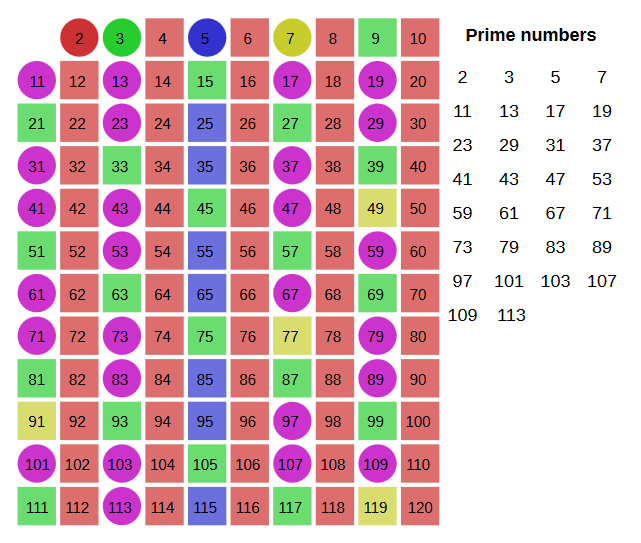
\includegraphics{figures/Primes-via-Eratosthenes-from-Wikipedia_en.png}
 }
% footnotemark, damit Nummer direkt hinter dem Titel; protect davor, um Compilierungsfehler
% zu vermeiden (http://www.undertec.de/blog/2013/06/latex-error-argument-of-caption-has-an-extra.html),
 % da es ein fragile command. footnotetext NACH end{figure}, sonst Fußnote nicht angezeigt.
 \caption[Das Sieb des Eratosthenes angewandt auf die ersten 120 Zahlen]
         {Das Sieb des Eratosthenes angewandt auf die ersten 120 Zahlen\protect\footnotemark}
\label{SieveEratosthenes01-figure}
\end{center}
\end{figure}
\footnotetext{%
   Grafik von
   \url{https://upload.wikimedia.org/wikipedia/commons/0/0b/Sieve_of_Eratosthenes_animation.svg}
   }

Durchzuführen braucht man das nur bis zu der größten Zahl,
deren Quadrat kleiner oder gleich $x$ ist (hier also bis 10, da $11^2$ schon $> 120$).%
\footnote{%
\index{ZT, Lernprogramm Zahlentheorie}%
\index{Lernprogramm ZT}%
Mit dem Lernprogramm \textbf{ZT} können Sie für beliebige eigene Wertemengen
das Sieb des Eratosthenes rechnergestützt und geführt Schritt für
Schritt anwenden: Siehe ZT-Lern-Kapitel 1.2, Seite 6/21 und 7/21.\\
ZT können Sie in CT1\index{CT1} über das Menü
\textbf{Einzelverfahren \textbackslash{} Zahlentheorie interaktiv \textbackslash{}
Lernprogramm für Zahlentheorie} aufrufen.
    Siehe Anhang \ref{s:appendix-Learn-NT}.\\
    Eine Visualisierung dieses Verfahrens ist in CT2\index{CT2}
    in dem Tutorial \textbf{\glqq Die Welt der Primzahlen\grqq}~enthalten.
}


Abgesehen von 2 sind Primzahlen nie gerade. Abgesehen von 2 und 5 haben Primzahlen nie die
Endziffern 2, 5 oder 0. Also braucht man sowieso nur Zahlen mit den Endziffern 1, 3, 7, 9 zu
betrachten (es gibt unendlich viele Primzahlen mit jeder dieser letzten Ziffern; vergleiche
\cite[Bd. 1, S. 137]{Tietze1973}).

Inzwischen findet man im Internet große Datenbanken, die entweder viele
Primzahlen oder die Zerlegung vieler zusammengesetzter Zahlen
in ihre Primfaktoren enthalten.


\paragraph*{Weitere interessante Themen rund um Primzahlen} \mbox{}\\
In diesem Kapitel \ref{Chapter_Primes} wurden weitere, eher zahlentheoretische
Themen wie Teilbarkeitsregeln, Modulo-Rechnung, modulare Inverse, modulare Potenzen
und Wurzeln, chinesischer Restesatz, Eulersche Phi-Funktion und perfekte Zahlen
nicht betrachtet. Auf einige dieser Themen geht das \hyperlink{Chapter_ElementaryNT}
{\textbf{nächste Kapitel}} (Kapitel \ref{Chapter_ElementaryNT}) ein.



% --------------------------------------------------------------------------
\pagebreak
\hypertarget{h_Notes-about-primes}{}
\section{Anmerkungen zu Primzahlen}
\label{l_Notes-about-primes}

Die folgenden Anmerkungen listen einzelne interessante Sätze, Vermutungen und
Fragestellungen zu Primzahlen auf, aber auch Kurioses und Übersichten.


% --------------------------------------------------------------------------
\vskip +20 pt
\subsection{Bewiesene Aussagen / Sätze zu Primzahlen}
\begin{itemize}

  \item Zu jeder Zahl $n$ aus $\textbf{N}$ gibt es $n$ aufeinanderfolgende
     natürliche Zahlen, die keine Prim"-zahlen sind.
     Ein Beweis findet sich in \cite[S. 79]{Padberg1996}.


  \item Paul Erdös\footnote{%
        Paul Erdös\index{Erdös, Paul}, ungarischer Mathematiker,
        26.03.1913$-$20.09.1996. }
     bewies:
     Zwischen jeder beliebigen Zahl ungleich $1$ und ihrem Doppelten gibt
     es mindestens eine Primzahl. Er bewies das Theorem nicht als erster,
     aber auf einfachere Weise als andere vor ihm.


  \item % \hypertarget{link-Primzahlfunktion-base-a-Proof}{}
        \label{link-Primzahlfunktion-base-a-Proof}
     Es existiert eine reelle Zahl a, so dass die Funktion
     $f: \textbf{N} \rightarrow {\mathbb Z}$ mit $n \mapsto \lfloor a^{3^n}\rfloor$
     für alle $n$ nur Primzahlenwerte annimmt\footnote{%
     Die Gaussklammer \index{Gaussklammer} $\lfloor x \rfloor $ der
     reellwertigen Zahl $x$ ist definiert als: $\lfloor x \rfloor $ ist die
     größte ganze Zahl kleiner oder gleich $x$.
     } (siehe \cite[S. 82]{Padberg1996}).
     Leider macht die Bestimmung von $a$ Probleme (siehe Kapitel
     \ref{link-Primzahlfunktion-base-a-Offen}).\footnote{%
     Wenn jemand weiß, wie man das beweist, würden wir uns sehr freuen, dies
     zu erfahren. Friedhelm Padberg sagte auf Nachfrage, er habe den
     Beweis nicht mehr.}

% \label{zahlentyp_mersenne}
% \hypertarget{GIMPS-project}{}
% \hyperlink{GIMPS-project}{GIMPS-Projekt} (Kapitel~\ref{zahlentyp_mersenne}),


  \vskip +6 pt
  \item \hypertarget{link-Arithmetic-sequence-of-primes}{}
     Es gibt arithmetische Primzahlfolgen \index{Primzahlfolge!arithmetische}
     beliebig großer Länge.\footnote{%
     Quellen: \\
     - \url{http://primes.utm.edu/glossary/page.php?sort=ArithmeticSequence}
         ~~~Original-Quelle\\
     - \url{http://en.wikipedia.org/wiki/Primes_in_arithmetic_progression}\\
     - \url{http://en.wikipedia.org/wiki/Problems_involving_arithmetic_progressions}\\
     - \url{https://de.wikipedia.org/wiki/Cunningham-Kette}\\
     - GEO 10 / 2004: \glqq Experiment mit Folgen\grqq\\
     - \url{http://www.faz.net}
       \glqq Hardys Vermutung -- Primzahlen ohne Ende\grqq~von Heinrich Hemme (06. Juli 2004)
     }$^,$\footnote{%  Doppelfussnote
     Arithmetische Folgen mit k Primzahlen werden auch Prime arithmetic progressions
     genannt und daher PAP-k bzw. AP-k abgekürzt.
     }

     Die 1923 von dem berühmten englischen Mathematiker Hardy\footnote{%
     Godfrey Harold Hardy\index{Hardy, Godfrey Harold}, britischer
     Mathematiker, 7.2.1877$-$1.12.1947.}
     aufge"-stellte Vermutung, dass es arithmetische Folgen beliebiger Länge
     gibt, die nur aus Prim"-zahlen bestehen, wurde 2004 von zwei jungen
     amerikanischen Mathematikern bewiesen.

     Jedes Schulkind lernt im Mathematikunterricht irgendwann einmal die
     arithmetischen Zahlenfolgen kennen. Das sind Aneinanderreihungen von
     Zahlen, bei denen die Abstände zwischen je zwei aufeinander folgenden
     Gliedern gleich sind - etwa bei der Folge 5, 8, 11, 14, 17, 20. Der
     Abstand der Glieder beträgt hierbei jeweils 3 und die Folge hat 6
     Folgenglieder. Eine arithmetische Folge muss mindestens 3 Folgenglieder
     haben, kann aber auch unendlich viele haben.

     Arithmetische Folgen sind seit Jahrtausenden bekannt und bergen eigentlich
     keine Ge"-heim"-nisse mehr.
     Spannend wird es erst wieder, wenn die Glieder einer arithmetischen Folge
     noch zusätzliche Eigenschaften haben sollen, wie das bei Primzahlen der
     Fall ist.

     Primzahlen sind ganze Zahlen, die größer als 1 und nur durch 1 und sich
     selbst ohne Rest teilbar sind. Die zehn kleinsten Primzahlen sind
     2, 3, 5, 7, 11, 13,  17, 19, 23 und 29.

     Eine arithmetische Primzahlfolge mit fünf Gliedern ist beispielsweise
     5, 17, 29, 41, 53. Der Abstand der Zahlen beträgt jeweils 12.

     Diese Folge lässt sich nicht verlängern, ohne ihre Eigenschaft
     einzubüßen, denn das nächste Glied müsste 65 sein, und diese Zahl ist
     das Produkt aus 5 und 13 und somit keine Primzahl.

     Wie viele Glieder kann eine arithmetische Primzahlfolge haben? Mit dieser
     Frage haben sich schon um 1770 der Franzose Joseph-Louis Lagrange und der
     Engländer Edward Waring beschäftigt. Im Jahre 1923 vermuteten der
     berühmte britische Mathematiker Godfrey Harold Hardy und sein Kollege
     John Littlewood, dass es keine Obergrenze für die Zahl der Glieder gebe.
     Doch es gelang ihnen nicht, das zu beweisen. Im Jahr 1939 gab es jedoch
     einen anderen Fortschritt: Der holländische Mathematiker Johannes van der
     Corput konnte nachweisen, dass es unendlich viele arithmetische
     Primzahlfolgen mit genau drei Gliedern gibt. Zwei Beispiele hierfür sind
     3, 5, 7  und  47, 53, 59.

     Die längste Primzahlfolge, die man bisher kennt, hat 25 Glieder.
     In der Tabelle~\ref{Smallest AP-k with minimal difference}
     sind die längsten bekannten arithmetischen
     Primzahlfolgen mit minimaler Distanz\footnote{%
        Dagegen sind in
        \url{http://en.wikipedia.org/wiki/Primes_in_arithmetic_progression}
        die \glqq Largest known AP-k\grqq~aufgelistet.
        Also ist dort das letzte Folgenelement eine möglichst große Primzahl.\\
        Tabelle \ref{Smallest AP-k with minimal difference} listet jedoch die
	Folgen auf, die die kleinsten bekannten Differenzen haben -- für eine
	gegebene Folgenlänge.
     }
     aufgelistet.

     Den beiden jungen\footnote{%
     In seinen Memoiren hat Hardy\index{Hardy, Godfrey Harold} 1940 geschrieben,
     dass die Mathematik mehr als alle anderen Wissenschaften und Künste
     ein Spiel für junge Leute sei. \\
     Der damals 27 Jahre alte Ben Green von der University of British Columbia
     in Vancouver und der damals 29 Jahre alte Terence Tao\index{Tao, Terence} von der
     University of California in Los Angeles scheinen ihm recht zu geben.
     }
     Mathematikern  Ben Green and Terence Tao ist es im Jahre 2004 gelungen,
     die mehr als achtzig Jahre alte Hardysche Vermutung zu beweisen:
     Es gibt arithmetische Primzahlfolgen beliebiger Länge. Außerdem bewiesen
     sie, dass es zu jeder vorgegebenen Länge unendlich viele verschiedene
     solcher Folgen gibt.

     Eigentlich hatten Green und Tao nur beweisen wollen, dass es unendlich
     viele arithmetische Primzahlfolgen mit vier Gliedern gibt. Dazu
     betrachteten sie Mengen, die neben Primzahlen auch
     Beinaheprimzahlen\index{Beinaheprimzahl}\index{Primzahl!Beinaheprimzahl}
     enthielten. Das sind Zahlen, die nur wenige Teiler haben - beispielsweise
     die Halbprimzahlen%
     \index{Halbprimzahl}\index{Primzahl!Halbprimzahl}%
     \index{Zahlen!semiprim}\index{Zahlen!Halbprimzahl},
     die Produkte aus genau zwei Primzahlen sind.
     Dadurch konnten die beiden Mathematiker ihre Arbeit wesentlich
     erleichtern, denn über Beinaheprimzahlen gab es schon zahlreiche
     nützliche Theoreme. Schließlich erkannten sie, dass ihr Verfahren viel
     mächtiger ist, als sie selbst angenommen hatten, und sie bewiesen damit
     die Hardysche Vermutung.

     Der Beweis von Green und Tao umfasst immerhin 49 Seiten. Tatsächlich
     beliebig lange arithmetische Primzahlfolgen kann man damit aber nicht
     finden. Der Beweis ist nicht konstruktiv, sondern ein so genannter
     Existenzbeweis\index{Beweis!Existenzbeweis}\index{Beweis!konstruktiv}.
     Das heißt, die beiden Mathematiker haben \glqq nur\grqq~gezeigt, dass
     beliebig lange Folgen existieren, aber nicht, wie man sie findet.

     Das heißt, in der Menge der natürlichen Primzahlen gibt es zum Beispiel
     eine Folge von einer Milliarde Primzahlen, die alle den gleichen Abstand
     haben; und davon gibt es unendlich viele. Diese Folgen liegen aber sehr
     \glqq weit draußen\grqq.   %\glqq D\grqq~


     \begin{table}[ht]
     \begin{center}
     \begin{tabular}{|r|r|r|r|r|}
     \hline
     Elemente & Startelement & Abstand & Wann   & Entdecker \\
              &              &         & Digits &           \\ \hline

      3 &                   3 &                   2 &      & \\
        &                     &                     &    1 & \\
	&&&& \\

      4 &                   5 &                   6 &      & \\
        &                     &                     &    2 & \\
	&&&& \\

      5 &                   5 &                   6 &      & \\
        &                     &                     &    2 & \\
	&&&& \\

      6 &                   7 &                  30 & 1909 & G. Lenaire \\
        &                     &                     &    3 & \\
	&&&& \\

      7 &                   7 &                 150 & 1909 & G. Lenaire \\
        &                     &                     &    3 & \\

....... &                     &                     &      & \\
	&&&& \\

     21 & 28.112.131.522.731.197.609 &          9.699.690 & 2008 & Jaroslaw Wroblewski\\
        &                            &              $= 19\#$ &   20 & \\
	&&&& \\

     22 &        166.537.312.120.867 &     96.599.212.710 & 2006 & Markus Frind\\
        &                            &        = 9.959·19\# &   15 & \\
	&&&& \\

     23 &        403.185.216.600.637 &  2.124.513.401.010 & 2006 & Markus Frind,\\
        &                            &        = 9.523·23\# &   15 & \\
	&&&& \\

     24 &        515.486.946.529.943 & 30.526.020.494.970 & 2008 & Raanan Chermoni,\\
        &                            &      = 136.831·23\# &   16 & Jaroslaw Wroblewski\\
	&&&& \\

     25 &      6.171.054.912.832.631 & 81.737.658.082.080 & 2008 & Raanan Chermoni,\\
        &                            &      = 366.384·23\# &   16 & Jaroslaw Wroblewski\\

     \hline
     \end{tabular}
     \caption{Arithmetische Primzahlfolgen mit minimaler Distanz (Stand Aug. 2012)}
     \label{Smallest AP-k with minimal difference}
     \end{center}
     \end{table}
     \clearpage

     Wer solche Folgen entdecken möchte, sollte folgendes berücksichtigen.
     Die Länge der Folge bestimmt den Mindestabstand zwischen den einzelnen
     Primzahlen. Bei einer Folge mit $k=6$ Gliedern muss der Abstand 30 oder ein
     Vielfaches davon betragen. Die Zahl 30 ergibt sich als das Produkt aller
     Primzahlen, die kleiner als die Folgenlänge, also kleiner als 6, sind:
     $ 6\# = 5\# = 2 * 3 * 5 = 30 $.
     Noch ein Beispiel: $ 10\# = 7\# = 2 * 3 * 5 * 7 = 210$.
     Sucht man Folgen mit der Länge 15, so muss der
     Abstand mindestens $ 15\# = 13\# = 2 * 3 * 5 * 7 * 11 * 13 = 30.030 $ betragen.
     \index{Primzahl!k Primorial} \index{Primzahl!k\#}

     Daraus ergibt sich, dass die Folgenlänge beliebig groß sein kann, aber
     der Abstand kann nicht jede beliebige Zahl annehmen: es kann keine
     arithmetische Primzahlfolge mit dem Abstand $100$ geben, denn 100 ist
     nicht durch die Zahl 3 teilbar.

     \begin{table}[ht]
     \begin{center}
     \hspace*{1cm}\begin{tabular}{|r|r|}
     \hline
      k &                k\# \\ \hline
      2 &                 2 \\
      3 &                 6 \\
      5 &                30 \\
      7 &               210 \\
     11 &             2.310 \\
     13 &            30.030 \\
     17 &           510.510 \\
     19 &         9.699.690 \\
     23 &       223.092.870 \\
      \hline
     \end{tabular}
     \caption{Produkte der ersten Primzahlen $<= k$ (genannt k Primorial oder $k\#$)}
     \end{center}
     \end{table}


     \vskip +10 pt
     \textbf{Weitere Restriktion an die arithmetische Folge:}\\
     Sucht man arithmetische Primzahlfolgen,
     die die {\em zusätzliche} Bedingung erfüllen, dass alle Primzahlen
     in der Folge auch {\em direkt hintereinander} liegen (consecutive
     primes sequence\footnote{%
     Sie werden auch consecutive prime arithmetic progressions genannt
     und daher CPAP-k bzw. CAP-k abgekürzt.
     }), wird es noch etwas schwieriger. Auf der
     Webseite von Chris Caldwell\footnote{%
     \url{http://primes.utm.edu/glossary/page.php?sort=ArithmeticSequence}
     }
     finden Sie weitere Informationen: Die längste bekannte arithmetische
     Folge, die nur aus direkt hintereinander liegenden Primzahlen besteht
     (Stand Aug. 2012), hat die Länge $10$, der Abstand beträgt
     $$ 10\# = 7\# = 2 * 3 * 5 * 7 = 210 $$
     und sie startet mit der 93-stelligen Primzahl\\
     100 9969724697 1424763778 6655587969 8403295093 2468919004 1803603417 7589043417 0334888215 9067229719\\


\end{itemize}



% --------------------------------------------------------------------------
% \vskip +10 pt
\newpage
\subsection[Verschiedene unbewiesene Aussagen / Vermutungen / offene Fragestellungen zu Primzahlen]
           {Verschiedene unbewiesene Aussagen / Vermutungen / offene Fragestellungen zu Primzahlen\footnote{%
  In seinem populärwissenschaftlichen Buch \glqq Die Musik der Primzahlen\grqq~
  beschreibt Marcus du Sautoy, Mathematikprofessor in Oxford, wie sich die
  brillantesten mathematischen Köpfe mit verschiedenen Aspekten der Primzahlen
  beschäftigten. Dabei stellt er diese Menschen vor (Gauß, Euler, Riemann, Ramanujan,
  Gödel, Connes, ...) und widmet sich insbesondere der \glqq Riemannschen Vermutung\grqq.
  Siehe \cite{duSautoy2005}.\index{Riemannsche Vermutung}\\
  Einfache Erläuterungen und Literaturhinweise zur Riemannschen Vermutung findet man
  auch in {\em RSA \& Co. in der Schule}, NF Teil 4 \cite{Witten2010a}.\index{RSA \& Co. in der Schule}
}
}

\begin{itemize}
  \item Goldbach\footnote{%
     Christian Goldbach\index{Goldbach, Christian}, deutscher Mathematiker,
     18.03.1690$-$20.11.1764. }
     vermutete:
     Jede gerade natür"-liche Zahl größer $2$ lässt sich als die Summe
     zweier Primzahlen darstellen.\footnote{Vergleiche auch Kapitel
     \ref{L-GoldbachConjecture}.}


\item Riemann\footnote{%
        Bernhard Riemann\index{Riemann, Bernhard}, deutscher Mathematiker,
        17.9.1826$-$20.7.1866.
     }
     stellte eine wichtige, bisher unbewiesene Hypothese\footnote{%
        \url{http://de.wikipedia.org/wiki/Riemannsche_Vermutung}
     }
     über die Nullstellen der Riemannschen Zetafunktion auf, aus der auch eine
     verbesserte Restglied"-ab"-schät"-zung im Primzahlsatz (Verteilung von
     Primzahlen) folgt.\index{Riemannsche Vermutung}


\item Das Benfordsche Gesetz\label{primes:Benford-Law}\index{Benfordsches Gesetz}\footnote{%
        \url{http://de.wikipedia.org/wiki/Benfordsches_Gesetz}, \\
        \url{http://www.spiegel.de/wissenschaft/mensch/0,1518,632541,00.html},\\
        \url{http://arxiv.org/PS_cache/arxiv/pdf/0906/0906.2789v1.pdf}.%Evtl. auch v3.pdf
        }$^,$\footnote{%
        Didaktische Darstellungen zu Anwendungen von Benfords Gesetz finden sich
        unter:
        \begin{compactitem}
         \item Rüdeger Baumann: \glqq Ziffernanalyse zwecks Betrugsaufdeckung
              --- Beispiel für kompetenzorientierten und kontextbezogenen
              Informatikunterricht\grqq, \\
              in LOGIN, Informatische Bildung und Computer in der Schule,
              Nr. 154/155, 2008, S. 68-72
         \item Norbert Hungerbühler: \glqq Benfords Gesetz über führende
              Ziffern\grqq, März 2007,\\
              %% Link tot: \url{http://www.educ.ethz.ch/unt/um/mathe/ana/benford}
	      \url{https://www.ethz.ch/content/dam/ethz/special-interest/dual/educeth-dam/documents/Unterrichtsmaterialien/mathematik/Benfords%20Gesetz%20%C3%BCber%20f%C3%BChrende%20Ziffern%20(Artikel)/benford.pdf}
        \end{compactitem}
        %\vspace{-\baselineskip} % Nützte nichts im Deutschen. Nötig im Englischen.
        }
     gilt nicht für Primzahlen.

     Nach dem Benfordschen Gesetz sind die Ziffern
     in den Zahlen bestimmter empirischer Datensätze (z.B. über Einwohnerzahlen
     von Städten, Geldbeträge in der Buchhaltung, Naturkonstanten) ungleichmäßig
     verteilt: Z.B. ist die Ziffer \verb#1# viel häufiger die erste Ziffer
     einer Zahl als jede andere.

     Welche Datensätze diesem Gesetz gehorchen ist noch nicht vollständig
     geklärt. Timo Eckhardt untersuchte in seiner Diplomarbeit 2008 ausführlich
     Eigenschaften von Primzahlen. Unter anderem wurden alle Primzahlen bis
     7.052.046.499 mit verschiedenen Stellenwert-Basen dargestellt.

     Beim Vergleich der Basen 3 bis 10 ergab sich, dass die Abweichung von
     Benfords Gesetz bei der Basis 3 am geringsten ist. Für die Basis zehn
     besteht in etwa eine Gleichverteilung der ersten Ziffern. Bei der
     Untersuchung größerer Basen ergab sich, dass die Verteilung der ersten
     Ziffern von Basis zu Basis sehr starke Unterschiede aufweist.



\item % \hypertarget{link-Primzahlfunktion-base-a-Offen}{}
      \label{link-Primzahlfunktion-base-a-Offen}
    Der in Kapitel \ref{link-Primzahlfunktion-base-a-Proof} erwähnte Beweis zu
    der Funktion  $f: \: N \rightarrow Z$ mit $n \mapsto \lfloor a^{3^n}\rfloor$
    garantiert nur die Existenz einer
    solchen Zahl $a$.  Wie kann diese Zahl $a$ bestimmt werden, und wird sie
    einen Wert haben, so dass die Funktion auch von praktischem Interesse ist?


\item Gibt es unendlich viele Mersenne-Primzahlen?
   \index{Primzahl!Mersenne}\index{Mersenne!Mersenne-Primzahl}

\item Gibt es unendlich viele Fermatsche Primzahlen?


\item Gibt es einen Polynomialzeit-Algorithmus\index{Polynom} zur
   Zerlegung einer Zahl in ihre Primfaktoren (vgl. \cite[S. 167]{Klee1997})?
   Diese Frage kann man auf die folgenden drei Fragestellungen aufsplitten:
   \begin{itemize}
        \item Gibt es einen Polynomialzeit-Algorithmus, der entscheidet, ob
	   eine Zahl prim ist? \\
	   Diese Frage wurde durch den AKS-Algorithmus\index{AKS}
	   beantwortet (vgl.  Kapitel \ref{PrimesinP}, \glqq PRIMES in P\grqq:
	   Testen auf Primalität ist polynominal).
        \item Gibt es einen Polynomialzeit-Algorithmus, mit dem man
           feststellen kann, aus wievielen Primfaktoren eine zusammengesetzte
           Zahl besteht (ohne diese Primfaktoren zu berechnen)?
        \item Gibt es einen Polynomialzeit-Algorithmus, mit dem sich für
	   eine zusammengesetzte Zahl $n$ ein nicht-trivialer (d.h.
	   von $1$ und von $n$ verschiedener) Teiler von $n$ berechnen
	   lässt?\footnote{Vergleiche auch Kapitel \ref{RSABernstein}
	   und Kapitel \ref{nt:NoteFactorization}.}
   \end{itemize}

   Am Ende von Kapitel \ref{nt:NoteFactorization},
   Abschnitt \hyperlink{RSA-200-chap3}{RSA-200}
   können Sie die Größenordnungen ersehen, für die heutige Algorithmen
   bei Primzahltests\index{Primzahltest} und bei der
   Faktorisierung\index{Faktorisierung!Faktorisierungsrekorde} gute
   Ergebnisse liefern.

\end{itemize}



% --------------------------------------------------------------------------
\vskip +10 pt
\hypertarget{HT-GoldbachConjecture}{}
\subsection{Die Goldbach-Vermutung}
\label{L-GoldbachConjecture}

Hier soll noch etwas tiefer auf die
\textbf{Goldbach-Vermutung}\index{Goldbach-Vermutung}\footnote{%
        \url{http://de.wikipedia.org/wiki/Goldbachsche_Vermutung} }
eingegangen werden.


%\vskip +25 pt
\hypertarget{HT-WeakGoldbachConjecture}{}
%\paragraph*{Die schwache Goldbach-Vermutung\footnote{%
%   Sie wird auch \textbf{ungerade} oder \textbf{ternäre} Goldbach-Vermutung
%   genannt.
%   } }%
%\subsubsubsection{xxx} 3*sub kennt er nicht, deshalb vorher paragraph !
% Ohne [] vor der { lässt er footnote nicht zu!
\subsubsection[Die schwache Goldbach-Vermutung]%
   {Die schwache Goldbach-Vermutung\footnote{%
   Sie wird auch \textbf{ungerade} oder \textbf{ternäre} Goldbach-Vermutung
   genannt.
   } }%
\index{Goldbach-Vermutung!schwach}%
\label{L-WeakGoldbachConjecture}%
%\mbox{}

 Goldbach stellte 1742 in einem Brief an den Mathematiker Euler die Behauptung auf:

Jede \textbf{ungerade} natürliche Zahl größer als 5 ist als Summe von \textbf{genau drei} Primzahlen darstellbar.

Beispiele: $7 = 3 + 2 + 2$ oder $27 = 19 + 5 + 3$ oder $27 = 17 + 5 + 5$

 Diese Behauptung ist immer noch (seit über 250 Jahren) unbewiesen.

 Mit Computern ist die \textbf{schwache Goldbach-Vermutung} für alle
ungeraden natürlichen Zahlen einfach bis $4*10^{18}$ (Stand April 2012) bzw.
doppelt bis  $4*10^{17}$ (Stand Mai 2013) verifiziert.\footnote{%
Siehe \url{http://sweet.ua.pt/tos/goldbach.html} von Tomás Oliveira e Silva
     }

Aus früheren Arbeiten ist bekannt, dass die schwache Goldbach-Vermutung
für alle ungeraden Zahlen größer $e^{3100}\approx 2 \times 10^{1346}$ wahr ist.

Wie bei vielen berühmten Vermutungen in der Mathematik gibt es auch für die
Goldbach-Vermutung eine Reihe angeblicher Beweise, die aber von der
mathematischen Gemeinschaft (noch) nicht akzeptiert sind.\footnote{%
Einer davon ist in dem Paper von Shan-Guang Tan, das am 16. Okt. 2011 (v1)
veröffentlicht, und zuletzt am 20. Mai 2016 (v19) revidiert wurde. Es
behauptet, sogar die starke Goldbach-Vermutung zu beweisen.\\
v1 hat den Titel \glqq A proof of the Goldbach conjecture\grqq.\\
v19 hat den Titel \glqq On the representation of even numbers as the sum and
difference of two primes and the representation of odd numbers as the sum of
an odd prime and an even semiprime and the distribution of primes in short
intervals\grqq.\\
Siehe \url{http://arxiv.org/abs/1110.3465}.
   }

Eine Vorarbeit für einen Beweis könnte die
kürzlich\footnote{\url{http://arxiv.org/abs/1201.6656}, eingereicht am
31. Jan. 2012 (v1), letzte Änderung 3. Juli 2012 (v4)} vorgestellte Arbeit
von Terence Tao\index{Tao, Terence} von der University of California sein.
Er bewies, dass sich jede \textbf{ungerade} natürliche Zahl größer 1 als
Summe von \textbf{höchstens fünf} Primzahlen darstellen lässt.

Inzwischen gab es erhebliche Arbeiten an der schwachen Goldbach-Vermutung. Sie
kulminierten 2013 in der Behauptung von Harald Helfgott, die Vermutung komplett
für alle natürlichen Zahlen größer 7 bewiesen zu haben.\footnote{%
Helfgott, H.A. (2013): \glqq Major arcs for Goldbach's theorem\grqq.
\url{http://arxiv.org/abs/1305.2897}.\\
v4 seines 79-seitigen Papers (14. April 2014) besagt, dass der Beweis für alle
natürlichen Zahlen ab $10^{29}$ (statt bisher $10^{30})$ gilt. Und für alle
Zahlen bis $10^{30}$ behauptet er, dass er und David Platt den Beweis durch
Probieren am Computer erbrachten.
\\
% BE_8.8.18: URL nicht erreichbar: \url{http://truthiscool.com/prime-numbers-the-271-year-old-puzzle-resolved}.\\
\url{https://www.newscientist.com/article/dn23535-proof-that-an-infinite-number-of-primes-are-paired.html}.\\
\url{www.spiegel.de/wissenschaft/mensch/beweis-fuer-schwache-goldbachsche-vermutung-a-901111.html}.
}



%\vskip +25 pt
\hypertarget{HT-StrongGoldbachConjecture}{}
%\subsubsubsection{xxx} 3*sub kannte er nicht, deshalb paragraph !
\subsubsection[Die starke Goldbach-Vermutung]%
   {Die starke Goldbach-Vermutung\footnote{%
   Sie wird auch \textbf{gerade} oder \textbf{binäre} Goldbach-Vermutung
   genannt.
   } }%
\index{Goldbach-Vermutung!stark}%
\label{L-StrongGoldbachConjecture}%
%\mbox{}

 Goldbachs starke Primzahlhypothese wurde von Euler nach einem Briefwechsel mit Goldbach formuliert, und wird meist einfach als \textbf{die} Goldbach-Vermutung bezeichnet:

Jede \textbf{gerade} natürliche Zahl größer als 2 ist als Summe von \textbf{genau zwei} Primzahlen darstellbar.

Beispiele für Goldach-Zerlegungen: $8 = 5 + 3$ oder $28 = 23 + 5$

 Mit Computern ist die \textbf{Goldbach-Vermutung}\index{Goldbach-Vermutung}
     für alle geraden Zahlen bis $4*10^{18}$ (Stand Mai 2013) einfach
     verifiziert\footnote{%
     Dass die Goldbach-Vermutung wahr ist, d.h. für alle geraden
     natürlichen Zahlen größer als $2$ gilt, wird heute allgemein nicht
     mehr angezweifelt. Der Mathematiker Jörg Richstein\index{Richstein 1999}
     vom Institut für Informatik der Universität Gießen hat 1999 die geraden
     Zahlen bis 400 Billionen ($4*10^{14}$) untersucht (\cite{Richstein1999})
     und kein Gegenbeispiel gefunden.\\
     Inzwischen wurden noch umfangreichere Überprüngen bis vorgenommem: Siehe\\
     \url{http://sweet.ua.pt/tos/goldbach.html} von Tomás Oliveira e Silva, \\
     \url{http://de.wikipedia.org/wiki/Goldbachsche\_Vermutung},\\
     \url{http://primes.utm.edu/glossary/page.php/GoldbachConjecture.html}.\\
     % http://www.mscs.dal.ca/\~{}joerg/res/g-en.html
     Trotzdem ist das kein allgemeiner Beweis.\\
     Dass die Goldbach-Vermutung trotz aller Anstrengungen bis heute
     nicht bewiesen wurde, lässt Folgendes befürchten:
     Seit den bahnbrechenden Arbeiten des österreichischen Mathematikers
     Kurt Gödel\index{Gödel, Kurt} ist bekannt, dass nicht jeder wahre
     Satz in der Mathematik auch beweisbar ist (siehe
     \url{https://www.mathematik.ch/mathematiker/goedel.php}).
     Möglicherweise hat Goldbach also Recht, und trotzdem wird nie ein
     Beweis gefunden werden. Das wiederum lässt sich aber vermutlich auch
     nicht beweisen.
     },   % end_footnote
     aber allgemein noch nicht bewiesen.\footnote{%
     Der englische Verlag {\em Faber} und die amerikanische
     Verlagsgesellschaft {\em Bloomsbury} publizierten 2000 das 1992 erstmals
     veröffentlichte Buch \glqq Onkel Petros und die Goldbachsche
     Vermutung\grqq~ von Apostolos Doxiadis (deutsch bei
     Lübbe 2000 und bei BLT als Taschenbuch 2001). Es ist
     die Geschichte eines Mathematikprofessors, der daran scheitert, ein
     mehr als 250 Jahre altes Rätsel zu lösen.\\
     Um die Verkaufszahlen zu fördern, schrieben die beiden Verlage einen
     Preis von 1 Million USD aus, wenn jemand die Vermutung beweist --
     veröffentlicht in einer angesehenen mathematischen Fachzeitschrift
     bis Ende 2004.\\
     Erstaunlicherweise durften nur englische und amerikanische Mathematiker
     daran teilnehmen.
     }${}^,$\footnote{%
     Die Aussage, die der starken Goldbach-Vermutung bisher am nächsten kommt,
     wurde 1966 von Chen Jing-Run bewiesen -- in einer schwer nachvollziehbaren
     Art und Weise: Jede gerade Zahl größer 2 ist die Summe einer Primzahl und
     des Produkts zweier Primzahlen. Z.B. $20=5+3*5.$\\
     Die wichtigsten Forschungsergebnisse zur Goldbach-Vermutung sind
     zusammengefasst in dem von Wang Yuan herausgegebenen Band:
     \glqq Goldbach Conjecture\grqq, 1984, World Scientific Series in Pure
     Maths, Vol. 4.
     }${}^,$\footnote{%
     Gerade diese Vermutung legt nahe, dass wir auch heute noch nicht in
     aller Tiefe den Zusammenhang zwischen der Addition und der Multiplikation
     der natürlichen Zahlen verstehen.
     }  % end_footnote

Je größer eine gerade Zahl ist, umso mehr solcher binärer Goldbach-Zerlegungen lassen sich im Durchschnitt finden: Für $4$ gibt es nur eine Zerlegung $2 + 2$; bei $16$ sind es schon zwei, nämlich $3 + 13$ und $5 + 11$. Bei $100$ sind es sechs $3 + 97$, $11 + 89$, $17 + 83$, $29 + 71$, $41 + 59$, $47 + 53$.\footnote{%
   Vergleiche \url{http://www.spiegel.de/wissenschaft/mensch/primzahlraetsel-loesung-der-goldbachschen-vermutung-rueckt-naeher-a-833216.html}. Dieser Artikel gehört in die Reihe
   der gut lesbaren Numerator-Kolumnen in Spiegel-Online von Holger Dambeck.
% Andere gute Kolumne zu seinen Forschungsergebnissen: http://terrytao.wordpress.com/
% Andere Disk.: http://mathforum.org/kb/message.jspa?messageID=7818160
% http://www.ams.org/news/math-in-the-media/06-2012-media
% http://aperiodical.com/2012/02/every-odd-integer-larger-than-1-is-the-sum-of-at-most-five-primes/
% http://oumathclub.wordpress.com/category/on-the-web/page/2/
% Vgl.: http://oumathclub.wordpress.com/  press column
   }   % end_footnote




\vskip +35 pt %Größer gemacht als 15, damit die ff. Überschrift nicht alle am Seitenende
%\subsubsubsection{xxx} 3*sub kannte er nicht, deshalb paragraph !
\subsubsection{Zusammenhang zwischen den beiden Goldbach-Ver\-mutungen}%
%\mbox{}

 Wenn die starke Goldbach-Vermutung gilt, gilt auch die schwache (d.h. die starke impliziert die schwache Vermutung).

Der Beweis dafür ist relativ einfach:\\
Voraussetzung: Sei $u$ eine ungerade Zahl größer als $5$.\\
Jede solche ungerade Zahl $u$ kann als Summe
$u = (u-3) + 3$ geschrieben werden. Der erste Summand ist dann gerade und $>= 4$, erfüllt
damit die Voraussetzung der starken Goldbach-Vermutung und kann damit als Summe zweier
Primzahlen $p_1$ und $p_2$ geschrieben werden (wobei $p_1$ und $p_2$ nicht notwendigerweise verschieden sein müssen). Damit hat man eine Zerlegung von $u$ in die drei Primzahlen $p_1, p_2$ und $3$ gefunden.
D.h. man kann sogar immer eine Summe finden, in der einer der drei primen Summanden die Zahl $3$ ist.

Ähnlich einfach kann man zeigen, dass aus der schwachen Golfbach-Vermutung die
oben erwähnte Behauptung von Terence Tao folgt (beide gelten für ungerade
Zahlen):
\begin{itemize}	
   \item Für ungerade Zahlen $u>5$ folgt direkt aus der schwachen
      Goldbach-Vermutung, dass die Summe aus höchstens fünf Primzahlen besteht.
   \item Für die restlichen ungeraden Zahlen $3$ und $5$ kann man es direkt
      einsetzen:\\
      $3 = 3$ (die \glqq Summe\grqq~hat nur einen und damit höchstens
      fünf prime Summanden);\\
      $5 = 2 + 3$ (die Summe hat zwei und damit höchstens fünf prime Summanden).
\end{itemize}




% --------------------------------------------------------------------------
\vskip +35 pt
\hypertarget{HT-TwinCousinPrimes}{}
\subsection{Offene Fragen zu Primzahlzwillingen und Primzahl-Cousins}
\label{L-TwinCousinPrimes}

Primzahlzwillinge\index{Primzahlzwilling} sind Primzahlen, die genau den
Abstand 2 voneinander haben, zum Beispiel 5 und 7, oder 101 und 103,
oder $1.693.965 \cdot 2^{66.443} \pm 1$.

 Das größte heutzutage bekannte Primzahlzwillingspaar
\[3.756.801.695.685\cdot 2^{666.669} \pm 1\] wurde im
Dezember 2011 gefunden und hat $200.700$ Dezimalstellen.\footnote{%
   \url{http://primes.utm.edu/primes},
   \url{http://www.primegrid.com/download/twin-666669.pdf} }


 Offen ist:
\begin{itemize}
\item Gibt es unendlich viele oder eine begrenzte Anzahl von
      Primzahlzwillingen?\footnote{%
      Bemerkung: Primzahl-\textbf{Drillinge} gibt es dagegen nur eines: 3, 5, 7.
      Bei allen anderen Dreierpacks aufeinanderfolgender ungerader Zahlen ist
      immer eine durch 3 teilbar und somit keine Primzahl.
                                  }${}^,$\footnote{%
      Die Vermutung, dass es unendlich viele Primzahlzwillinge gibt, ist nicht
      selbstverständlich. Man weiß, dass bei großen Zahlen im Durchschnitt der
      Abstand zwischen Primzahlen immer weiter wächst und ca. 2,3 mal so groß
      ist wie die Anzahl der Dezimalstellen. Beispielsweise beträgt bei
      100-stelligen Dezimalzahlen der Abstand zwischen Primzahlen im
      Durchschnitt 230.
      Aber diese Aussage gilt nur für den Durchschnitt -- oft ist der Abstand
      viel größer, oft viel kleiner.
                                  }${}^,$\footnote{%
      \url{http://de.wikipedia.org/wiki/Primzahlzwilling}
      }

\item Gibt es eine Formel für die Anzahl der Primzahlzwillinge pro Intervall?
\end{itemize}

 Im Folgenden werden zwei größere Meilensteine erläutert, die dem
Rätsel näher kommen.


\subsubsection{GPY 2003}

Einen großen Schritt zur Klärung der ersten Frage machten möglicherweise
Dan Goldston, J\'{a}nos Pintz und Cem Yildirim im Jahre 2003.\footnote{%
    D. A. Goldston: \glqq Gaps Between Primes\grqq \\
    \url{http://www.math.sjsu.edu/~goldston/OberwolfachAbstract.pdf}\\
    Siehe auch:
    \begin{compactitem}
       \item D. A. Goldstone: \glqq Are There Infinitely Many Twin Primes?\grqq, \\
          \url{http://www.math.sjsu.edu/~goldston/twinprimes.pdf}
       \item K. Soundararajan: \glqq Small Gaps Between Prime Numbers:
           The Work Of Goldston-Pintz-Yildirim\grqq, \\
           \url{http://www.ams.org/bull/2007-44-01/S0273-0979-06-01142-6/S0273-0979-06-01142-6.pdf}
    \end{compactitem}
    \vspace{-\baselineskip} % TODO_LaTeX: Geht das nicht anders?
   }
Die drei Mathematiker beschäftigten sich mit der Verteilung von Primzahlen.
Sie konnten beweisen, dass  \[ \liminf_{n\to\infty}{\frac{p_{n+1}-p_n}{\log{p_n}}}=0,\]
wobei $p_{n}$ die $n$-te Primzahl bezeichnet. \\
Dies bedeutet, dass der kleinste Häufungspunkt ($\liminf$) der Folge
$\frac{p_{n+1}-p_n}{\log{p_n}}$ gleich Null ist.\\
Ein Punkt heißt Häufungspunkt einer Folge, wenn in jeder noch so kleinen
Umgebung um diesen Punkt unendlich viele Folgeglieder liegen. \\
$\log{p_n}$ ist in etwa der erwartete Abstand zwischen der Primzahl $p_n$
und der darauf folgenden Primzahl $p_{n+1}$.\\
Der obige Term besagt also, dass es unendlich viele aufeinander folgende
Primzahlen gibt, deren Abstand im Verhältnis zum erwarteten durchschnittlichen
Abstand beliebig nah an Null bzw. beliebig klein ist.

Außerdem konnte gezeigt werden, dass für unendlich viele Primzahlen
gilt\footnote{ c't 2003, Heft 8, Seite 54}: \[p_{n+1}-p_n < (\log{p_n})^{8/9}\]



\subsubsection{Zhang 2013}

Im Mai 2013 wurde die Arbeit von Yitang Zhang\index{Zhang, Yitang}
bekannt.\footnote{%
   Erica Klarreich (19. Mai 2013): \glqq Unheralded Mathematician Bridges the
   Prime Gap\grqq \\
   \url{https://www.quantamagazine.org/yitang-zhang-proves-landmark-theorem-in-distribution-of-prime-numbers-20130519/}}
   % BE _8.8.18: Alte URL, die auf die neue umgeleitet wurde: \url{https://www.simonsfoundation.org/quanta/20130519-unheralded-mathematician-bridges-the-prime-gap/}}
Zhang beweist, dass es unendlich viele \glqq Primzahl-Cousins\grqq~gibt, oder
genauer, dass es unendlich viele Primzahlpaare gibt, die einen Abstand von $H$
haben und dass die Zahl $H$ kleiner als 70 Millionen ist.\footnote{%
Während bei einem Primzahl-Zwilling der Abstand der beiden Primzahlen genau
$2$ ist, bezeichnen Primzahl-Cousins\index{Primzahl-Cousin} zwei Primzahlen,
deren Abstand den Wert einer größeren geraden, aber endlichen Zahl $H$ hat.
      }${}^,$\footnote{%
Dies ist nahezu der Beweis für die Vermutung, die 1849 von dem französichen
Mathematiker Alphonse de Polignac aufgestellt wurde, dass es unendlich viele
Primzahl-Paare gibt zu jeder möglichen geraden und endlichen Lücke (nicht nur
für die $2$).
       }${}^,$\footnote{%
In weiteren Arbeiten wurde dieser Mindestabstand $H$ von 70 Millionen
weiter verbessert. Diese Fortschritte werden im 8. Polymath-Projekt
(massively collaborative online mathematical projects) dokumentiert: "Bounded
gaps between primes". Der beste bisher bekannte Werte für $H$ war $4680$ (Stand
August 2013) und ist $246$ (Stand April 2014) -- das ist ein guter Fortschritt
gegenüber 70 Millionen, aber immer noch weit entfernt von $2$.\\
Siehe \url{http://michaelnielsen.org/polymath1/index.php?title=Bounded_gaps_between_primes}
%%% TODO-Check-Current-Research-xxxxx:
%%% Bester Wert (Mindestabstand unendlich vieler Primzahlzwillinge) = 246 laut
%%% http://www.golem.de/news/mathematik-er-denkt-nur-an-2-3-5-7-11-13-1607-122284.html vom 22.7.16
%%% http://www.magd.ox.ac.uk/member-of-staff/james-maynard/
%%% http://arxiv.org/abs/1311.4600, Small gaps between primes, James Maynard, 19 Nov 2013 --> 600
%%% https://en.wikipedia.org/wiki/James_Maynard_(mathematician)  --> 246:
%%% --> As of April 14, 2014, one year after Zhang's announcement, according to the
%%%     Polymath project wiki, N has been reduced to 246.
   }

Diese Aussagen könnten Grundlage sein um zu beweisen, dass es unendlich
viele Primzahl"-zwillinge gibt.



% --------------------------------------------------------------------------
%\vskip +25 pt
\newpage
% Die eckigen Klammern sind nötig, will man \footnotmark innerhalb der {}
% verwenden.
% Man muss den Titel sowohl in die [] als auch in die {} stellen:
% - Fehlt er innerhalb {}, ist die Überschrift innerhalb des Textes leer.
% - Fehlt er innerhalb [], fehlt die Überschrift links im PDF-Rahmen und
%   im Inhaltsverzeichnis.
\subsection[Kurioses und Interessantes zu Primzahlen]
              {Kurioses und Interessantes zu Primzahlen\footnotemark}
    \footnotetext{%
Weitere kuriose und seltsame Dinge zu Primzahlen finden sich auch unter:\\
- \url{http://primes.utm.edu/curios/home.php}\\
- \url{http://www.primzahlen.de}.
}
\label{HT-Quaint-curious-Primes-usage}

Primzahlen sind nicht nur ein sehr aktives und ernstes mathematisches
Forschungsgebiet. Mit ihnen beschäftigen sich Menschen auch hobbymäßig und
außerhalb der wissenschaftlichen For"-schung.


\vskip +25 pt
\hypertarget{HT-GoogleRecruitment2004}{}
\subsubsection{Mitarbeiterwerbung bei Google im Jahre 2004}
% \paragraph*{Mitarbeiterwerbung bei Google im Jahre 2004}%
\index{Google!Mitarbeiterwerbung}%
\label{HT-GoogleRecruitment2004}%
\mbox{}
Im Sommer 2004 benutzte die Firma Google die Zahl $e$, um Bewerber zu
gewinnen.\footnote{Die Basis des natürlichen Logarithmus\index{Logarithmus!natürlich}
$e$ ist ungefähr 2,718 281 828 459.
Dies ist eine der bedeutendsten Zahlen in der Mathematik. Sie wird gebraucht
für komplexe Analysis, Finanzmathematik, Physik und Geometrie. Nun wurde sie
-- meines Wissens -- das erste Mal für Marketing oder Personalbeschaffung
verwendet.}${}^,$\footnote{Die meisten Informationen für diesen Paragraphen
stammen aus dem Artikel \glqq e-number crunching\grqq~ von John Allen Paulos
in TheGuardian vom 30.09.2004 und aus dem Internet:\\
%% Veraltet, geht aber noch: \url{http://www.mkaz.com/math/google/}\\
- \url{https://mkaz.blog/math/google-billboard-problems/}\\
- \url{http://epramono.blogspot.com/2004/10/7427466391.html}\\
- \url{http://mathworld.wolfram.com/news/2004-10-13/google/}.
%% Nur zum Autor: \url{http://www.math.temple.edu/~paulos/}.
}

Auf einer hervorstechenden Reklamewand im kalifornischen Silicon Valley
erschien am 12. Juli das folgende geheimnisvolle Rätsel:
\begin{center}
{\em  (first 10-digit prime found in consecutive digits of e).com  }
\end{center}
In der Dezimaldarstellung von $e$ sollte man also die erste 10-stellige Primzahl
finden, die sich in den Nachkommastellen befindet. Mit verschiedenen
Software-Tools kann man die Antwort finden:
$$ 7.427.466.391 $$

Wenn man dann die Webseite $www.7427466391.com$ besuchte, bekam man ein noch
schwie"-rigeres Rätsel gezeigt. Wenn man auch dieses zweite Rätsel löste, kam
man zu einer weiteren Webseite, die darum bat, den Lebenslauf an Google zu
senden. Diese Werbekampagne erzielte eine hohe Aufmerksamkeit.

Wahrscheinlich nahm Google an, dass man gut genug ist, für sie zu arbeiten, wenn
man diese Rätsel lösen kann. Aber bald konnte jeder mit Hilfe der Google-Suche
ohne Anstrengung die Antworten finden, weil viele die Lösung der Rätsel ins
Netz gestellt hatten.\footnote{%
Im zweiten Level der Rätsel musste man das 5. Glied einer gegebenen
Zahlenfolge finden: Dies hatte nichts mehr mit Primzahlen zu tun.}



\vskip +25 pt
\hypertarget{HT-Movie-Contact01}{}
\subsubsection{Contact [Film, 1997] -- Primzahlen zur Kontaktaufnahme}
% \paragraph*{xxx}
\index{Filme}\index{Zemeckis 1997}
\label{HT-Movie-Contact01}%
\mbox{}
Der Film von Regiseur Robert Zemeckis entstand nach dem gleichnamigen Buch von
Carl Sagan.

Die Astronomin Dr. Ellie Arroway (Jodie Foster) entdeckt nach jahrelanger vergeblicher
Suche Signale vom 26 Lichtjahre entfernten Sonnensystem Wega.
In diesen Signalen haben Außerirdische die Primzahlen lückenlos in der richtigen
Reihenfolge verschlüsselt. Daran erkennt die Heldin, dass diese Nachricht anders
ist als die ohnehin ständig auf der Erde eintreffenden Radiowellen, die
kosmischer und zufälliger Natur sind (von Radiogalaxien, Pulsaren oder Quasaren).
In einer entlarvenden Szene fragt sie daraufhin ein Politiker, warum diese
intelligenten Wesen nicht gleich Englisch sprechen ...

Eine Kommunikation mit absolut fremden und unbekannten Wesen aus dem All ist
aus 2 Gründen sehr schwierig:
Zunächst kann man sich bei der hier angenommenen Entfernung und dem damit
verbundenen langen Übertragungsweg in einem durchschnittlichen Menschenleben
nur einmal in jeder Richtungen nacheinander austauschen.
Zum Zweiten muss man für den Erstkontakt darauf achten, dass eine möglichst
hohe Chance besteht, dass der Empfänger der Radiowellen die Botschaft überhaupt
bemerkt und dass er sie als Nachricht von intelligenten Wesen einstuft.
Deshalb senden die Außerirdischen am Anfang ihrer Nachricht Zahlen, die als
der einfachste Teil jeder höheren Sprache angesehen werden können  und die nicht
ganz trivial sind: die Folge der Primzahlen. Diese speziellen Zahlen spielen in der
Mathematik eine so fundamentale Rolle, dass man annehmen kann, dass sie jeder
Spezies vertraut sind, die das technische Know-how hat, Radiowellen zu
empfangen.

Die Aliens schicken danach den Plan zum Bau einer mysteriösen Maschine ...



% --------------------------------------------------------------------------
\newpage
\hypertarget{primhfk}{}
\section{Anhang: Anzahl von Primzahlen in verschiedenen Intervallen}
\label{s:primhfk}
\vskip +10 pt

\begin{table}[ht]
\begin{center}
\begin{tabular}{|l|l||l|l||l|l|}\hline
\multicolumn{2}{|l||}{Zehnerintervall} & \multicolumn{2}{l||}{Hunderterintervall} & \multicolumn{2}{l|}{Tausenderintervall} \\ \hline
Intervall  &     Anzahl &    Intervall  &  Anzahl &  Intervall  &    Anzahl\\ \hline \hline
1-10     &       4     &     1-100   &     25  &     1-1.000     &    168 \\
11-20    &       4     &     101-200 &     21  &     1.001-2.000  &    135 \\
21-30    &       2     &     201-300 &     16  &     2.001-3.000  &    127  \\
31-40    &       2     &     301-400 &     16  &     3.001-4.000  &    120 \\
41-50    &       3     &     401-500 &     17  &     4.001-5.000  &    119 \\
51-60    &       2     &     501-600 &     14  &     5.001-6.000  &    114 \\
61-70    &       2     &     601-700 &     16  &     6.001-7.000  &    117 \\
71-80    &       3     &     701-800 &     14  &     7.001-8.000  &    107 \\
81-90    &       2     &     801-900 &     15  &     8.001-9.000  &    110 \\
91-100   &       1     &     901-1.000 &     14 &     9.001-10.000 &    112 \\ \hline
\end{tabular}
\caption{Wieviele Primzahlen gibt es innerhalb der ersten Zehner-/Hunderter-/Tausender-Intervalle?}
\end{center}
\end{table}
\vskip +20 pt


\begin{table}[ht]
\begin{center}
\begin{tabular}{|l|r|r|r|}\hline
Dimension & Intervall & Anzahl & Durchschnittl. Anzahl pro 1000 \\ \hline
  4  &  1 - 10.000           &   1.229       &    122,900 \\
  5  &  1 - 100.000          &   9.592       &     95,920 \\
  6  &  1 - 1.000.000        &   78.498      &     78,498 \\
  7  &  1 - 10.000.000       &   664.579     &     66,458 \\
  8  &  1 - 100.000.000      &   5.761.455   &     57,615 \\
  9  &  1 - 1.000.000.000    &   50.847.534  &     50,848 \\
 10  &  1 - 10.000.000.000   &   455.052.512 &     45,505 \\ \hline
\end{tabular}
\caption{Wieviele Primzahlen gibt es innerhalb der ersten Dimensionsintervalle?}
\end{center}
\end{table}
\vskip +6 pt

Eine Visualisierung der Anzahl von Primzahlen in höheren Intervallen von
Zehnerpotenzen finden Sie in Kapitel \ref{primes:_Appendix_Plotting-Primes-Quantity}
auf Seite \pageref{primes:_Appendix_subsubsection_NumberofPrimes-in-intervals}.



% --------------------------------------------------------------------------
\newpage
\hypertarget{ntePrimzahl}{}
\section{Anhang: Indizierung von Primzahlen (\texorpdfstring{$n$}{n}-te Primzahl)}
\label{s:ntePrimzahl}
\vskip +10 pt

\begin{table}[ht]
\begin{center}
\begin{tabular}{|l|l|l|l|}\hline
Index   &   Genauer Wert  &       Gerundeter Wert &    Bemerkung \\
\hline \hline
1       &   2             &     2  & \\
2       &   3             &     3  &  \\
3       &   5             &     5  & \\
4       &   7             &     7  & \\
5       &   11            &     11 & \\
6       &   13            &     13 & \\
7       &   17            &     17 & \\
8       &   19            &     19 & \\
9       &   23            &     23 & \\
10      &   29            &     29 & \\
100     &   541           &     541 & \\
1000    &   7917          &     7917 & \\
664.559  &  9.999.991     &     9,99999E+06 & Alle Primzahlen bis zu 1E+07 waren am\\
         &                &                 & Beginn des 20. Jahrhunderts bekannt.\\
1E+06  &    15.485.863   &      1,54859E+07 & \\
6E+06  &    104.395.301    &    1,04395E+08  & Diese Primzahl wurde 1959 entdeckt.\\
1E+07  &    179.424.673     &    1,79425E+08 & \\
1E+09  &    22.801.763.489  &    2,28018E+10 & \\
1E+12  &    29.996.224.275.833 & 2,99962E+13 & \\ \hline
\end{tabular}
\caption{Liste selektierter $n$-ter Primzahlen P(n)}\index{P(n)}
\end{center}
\end{table}


\vskip +10pt
\begin{remark}{:} Mit Lücke wurden früh sehr große Primzahlen entdeckt. \\
\end{remark}

\vskip +12pt
 \textbf{Web-Links (URLs):}\\
\url{https://primes.utm.edu/nthprime/} \\
\url{https://primes.utm.edu/notes/by_year.html}.



% --------------------------------------------------------------------------
\newpage
\section{Anhang: Größenordnungen / Dimensionen in der Realität}
\label{s:grosord}
Bei der Beschreibung kryptographischer Protokolle und Algorithmen
treten Zahlen auf, die so groß bzw. so klein sind, dass sie einem
intuitiven Verständnis nicht zugänglich sind. Es kann daher
nützlich sein, Vergleichszahlen aus der uns umgebenden realen
Welt bereitzustellen, so dass man ein Gefühl für die Sicherheit
kryptographischer Algorithmen entwickeln kann. Die angegebenen
Werte stammen größtenteils aus \cite{Schwenk1996} und
\cite[S.18]{Schneier1996}.  \hypertarget{grosord}{}

% be_2005: noch mit tabbing:
% Wahrscheinlichkeit, dass Sie auf ihrem nächsten Flug entführt werden:	&~~ \= abcdefhijk \= \kill
% Wahrscheinlichkeit, dass Sie auf ihrem nächsten Flug entführt werden \> $ 5,5 \cdot 10^{-6} $\> \\

\vskip +20pt
\begin{table}[ht]
\begin{center}
\begin{tabular}{|l|l|}\hline
Wahrscheinlichkeit, dass Sie auf ihrem nächsten Flug entführt werden	&  $ 5,5 \cdot 10^{-6} $  \\
Jährliche Wahrscheinlichkeit, von einem Blitz getroffen zu werden	&  $ 10^{-7} $            \\
Wahrscheinlichkeit für 6 Richtige im Lotto				&  $ 7,1 \cdot 10^{-8} $  \\
Risiko, von einem Meteoriten erschlagen zu werden			&  $ 1,6 \cdot 10^{-12} $ \\
\hline
Zeit bis zur nächsten Eiszeit (in Jahren)	&  $14.000 $   =  $(2^{14})$ \\
Zeit bis die Sonne verglüht (in Jahren)	&  $10^{9} $   =  $(2^{30})$ \\
Alter der Erde (in Jahren)			&  $ 10^9 $    =  $(2^{30})$ \\
Alter des Universums (in Jahren)		&  $ 10^{10} $ =  $(2^{34})$ \\
Anzahl der Moleküle in einem Wassertropfen	&  $10^{20} $  =  $(2^{63})$ \\
Anzahl der auf der Erde lebenden Bakterien	&  $10^{30,7} $ = $(2^{102})$ \\
%Quelle: ISBN 3-7776-1258-8 Küssen müssen wir noch lernen + Hummer haben blaues Blut, Herzel-Verlag
Anzahl der Atome der Erde 			&  $10^{51} $  =  $(2^{170})$ \\
Anzahl der Atome der Sonne			&  $10^{57}$   =  $(2^{190})$ \\
Anzahl der Atome im Universum (ohne dunkle Materie)	&  $10^{77}$  = $(2^{265})$ \\
Volumen des Universums (in $cm^3$)		&  $10^{84}$   = $(2^{280})$ \\ \hline
\end{tabular}
\caption{Wahrscheinlichkeiten und Größenordnungen aus Physik und Alltag}
\end{center}
\end{table}


% --------------------------------------------------------------------------
\newpage
\section{Anhang: Spezielle Werte des Zweier- und Zehnersystems}

Diese Werte können dazu benutzt werden, aus einer Schlüssellänge in Bit
die Anzahl möglicher Schlüssel und den Such-Aufwand abzuschätzen (wenn man
z.B. annimmt, dass 1 Million Schlüs"-sel in 1 sec durchprobiert werden können).

% be_2005 vorher nur getappt, nun als Tabelle mit Rahmen
% \begin{tabbing}
% DualSystem~~~ \= \kill
% Dualsystem \> Zehnersystem \\*[4pt]
% $2^{10}$ \> $1024$ \\
% ...
% $2^{2048}$ \>   $3,23170\cdot 10^{616}$ \\
% \end{tabbing}

\begin{table}[ht]
\begin{center}
\begin{tabular}{|l|l|}\hline
Dualsystem   &   Zehnersystem \\
\hline \hline
$2^{10}$ 	&   $1024$ \\
$2^{40}$ 	&   $1,09951\cdot 10^{12}$ \\
$2^{56}$ 	&   $7,20576\cdot 10^{16}$ \\
$2^{64}$ 	&   $1,84467\cdot 10^{19}$ \\
$2^{80}$ 	&   $1,20893\cdot 10^{24}$ \\
$2^{90}$ 	&   $1,23794\cdot 10^{27}$ \\
$2^{112}$ 	&   $5,19230\cdot 10^{33}$ \\
$2^{128}$ 	&   $3,40282\cdot 10^{38}$ \\
$2^{150}$ 	&   $1,42725\cdot 10^{45}$ \\
$2^{160}$ 	&   $1,46150\cdot 10^{48}$ \\
$2^{192}$ 	&   $6,27710\cdot 10^{57}$ \\
$2^{250}$ 	&   $1,80925\cdot 10^{75}$ \\
$2^{256}$ 	&   $1,15792\cdot 10^{77}$ \\
$2^{320}$ 	&   $2,13599\cdot 10^{96}$ \\
$2^{512}$ 	&   $1,34078\cdot 10^{154}$ \\
$2^{768}$ 	&   $1,55252\cdot 10^{231}$ \\
$2^{1024}$ 	&   $1,79769\cdot 10^{308}$ \\
$2^{2048}$ 	&   $3,23170\cdot 10^{616}$ \\ \hline
\end{tabular}
\caption{Spezielle Werte des Zweier- und Zehnersystems}
\end{center}
\end{table}

Solche Tabellen lassen sich mit Computer-Algebra-Systemen einfach berechnen.
Hier ein Codebeispiel für das CAS-System SageMath\index{SageMath}\index{CAS}:

\begin{sagecode}
\begin{Verbatim}%
[fontsize=\footnotesize]
E = [10, 40, 56, 64, 80, 90, 112, 128, 150, 160, 192, 256, 1024, 2048]
for e in E:
    # print "2^" + str(e), "---", 1.0*(2^e)
    print "2^%4d" % e , " --- ", RR(2^e).n(24)
....:
2^  10  ---  1024.00
2^  40  ---  1.09951e12
2^  56  ---  7.20576e16
2^  64  ---  1.84467e19
2^  80  ---  1.20893e24
2^  90  ---  1.23794e27
2^ 112  ---  5.19230e33
2^ 128  ---  3.40282e38
2^ 150  ---  1.42725e45
2^ 160  ---  1.46150e48
2^ 192  ---  6.27710e57
2^ 256  ---  1.15792e77
2^1024  ---  1.79769e308
2^2048  ---  3.23170e616
\end{Verbatim}
\caption{Spezielle Werte des Zweier- und Zehnersystems}
\end{sagecode}






% ---------------------------------------------------------------------------
% ---------------------------------------------------------------------------
\newpage
\hypertarget{primes:_Appendix_Plotting-Primes-Quantity}{}
\section{Anhang: Visualisierung der Menge der Primzahlen in hohen Bereichen}
\label{primes:_Appendix_Plotting-Primes-Quantity}
\index{SageMath!Programmbeispiele}
\index{SageMath}
\vskip +15pt

% ---------------------------------------------------------------------------
\subsection*{Zur Verteilung von Primzahlen}
Zwischen $1$ und $10$ gibt es $4$ Primzahlen. Zwischen $10^3$ und $10^4$ sind
es schon $1061$. Im Intervall $[10^9,10^{10}]$ liegen
$404.204.977\approx 4\cdot 10^{8}$ Primzahlen, und in dem Intervall von
$10^{19}$ bis $10^{20}$ sind es schon $1.986.761.935.284.574.233\approx 1,9\cdot 10^{18}$
Primzahlen.\footnote{\url{http://de.wikipedia.org/wiki/Primzahlsatz}}

Warum unterscheidet sich die Anzahl der Primzahlen, die in den verschiedenen
Intervallen liegen so stark, obwohl sich die Intervallgrenzen jeweils nur um
den Wert 1 im Exponenten der $10$-er Potenz unterscheiden?


\subsubsection*{Primzahlsatz}
Die Anzahl der Primzahlen PI(x) bis zu einer gegebenen Zahl $x$ kann durch
eine Formel nach dem sogenannten Primzahlsatz näherungsweise bestimmt werden
(siehe Kapitel \ref{l_Primes_Distrib-of-Primes}).
$PI(x)$ bezeichnet die Anzahl der Primzahlen kleiner oder gleich der Zahl $x$.
Dann lautet die Formel
\[PI(x)\sim \frac{x}{\ln{x}}.\]
\index{PI(x), $\Pi(x)$}
Es ist zu beachten, dass diese Formel die Anzahl der Primzahlen kleiner oder gleich $x$ nur
ungefähr angibt. Sie wird jedoch genauer je größer $x$ wird.
Im folgenden wollen wir den Primzahl"-satz nutzen, um uns die Verteilung der Primzahlen anzusehen.

Um zu verstehen, warum die Anzahl der Primzahlen so schnell wächst, obwohl sich
die Intervallgrenzen jeweils nur um einen Exponentenwert von 1  unterscheiden,
werfen wir einen Blick auf beide Komponenten der rechten Seite der Formel:
$x$ und $\ln{x}$.


\subsubsection*{Die Funktionen $x$ und $10^x$}
Die Funktion $x$ ist eine Gerade. Sie ist in Abbildung \ref{x} auf Seite \pageref{x} zu sehen.\\
Als nächstes tragen wir die Funktion der Intervallgrenzen in einem Graphen ab, der in
Abbildung \ref{10hochx} auf Seite \pageref{10hochx} zu finden ist. Um einen Eindruck zu
bekommen, wie die Funktionen aussehen, wurde der Definitionsbereich von $0$ bis $10^{10}$
bzw. entprechend von $0$ bis $10$ gewählt.
Es ist zu sehen, dass mit steigendem Exponenten $x$ die Zahlen immer größer werden.

\begin{figure}[!htb]
	\centering
	\subfloat[$x$]{\label{x}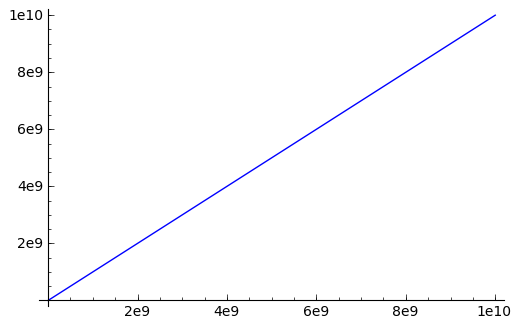
\includegraphics[height=4cm]{figures/x.png}}
	\hfill
	\subfloat[$10^x$]{\label{10hochx}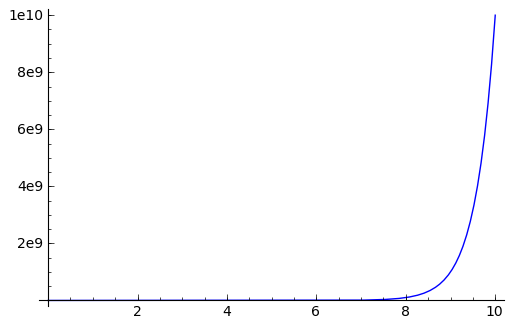
\includegraphics[height=4cm]{figures/10hochx.png}}
	\caption{Graph der Funktionen $x$ und $10^x$}
	\label{xund10hochx}
        \vskip +25pt
\end{figure}
% \\ nach end{figure} führt zu  LaTeX Error: There's no line here to end.
% \vskip +30pt  nach end{figure} stellt den Space an den falschen Ort, da die Grafik eigenständig gesetzt wird.
% \clearpage


\subsubsection*{Die Funktion $\ln{x}$}
Im Vergleich dazu betrachten wir die Funktion $\ln{x}$.
Auf dem linken Bild von Abbildung \ref{lnxbis} auf Seite \pageref{lnxbis} wurde der
Definitionsbereich von $1$ bis $100$ gewählt. Das rechte Bild zeigt die Werte der
Funktion bis $10^{10}$.\\
Es ist gut zu erkennen, dass die Werte der Funktion $\ln{x}$ im Vergleich zu $x$
langsam wachsen. Dies verdeutlicht auch der Graph beider Funktionen in Abbildung
\ref{xundlnxundxdurchlnx} auf Seite \pageref{xundlnxundxdurchlnx}. Zudem wurde
in diesen Graphen auch die Funktion $\frac{x}{\ln{x}}$ eingezeichnet.

\begin{figure}[!htb]
	\centering
	\subfloat[ ]{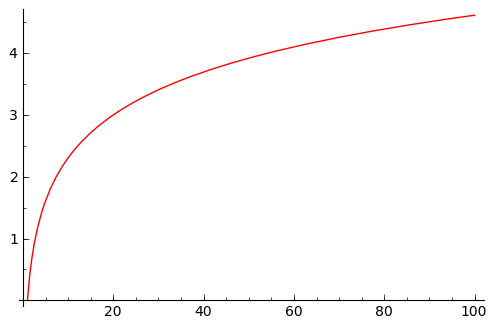
\includegraphics[height=4cm]{figures/lnxbis100.png}}
	\hfill
	\subfloat[ ]{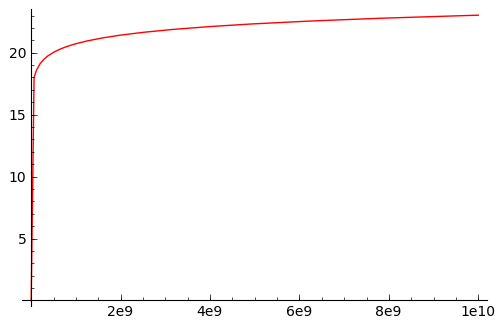
\includegraphics[height=4cm]{figures/lnxbis10hoch10.png}}
	\caption{Graph der Funktion $\ln{x}$ bis $100$ und bis $10^{10}$}
	\label{lnxbis}
        \vskip +25pt
\end{figure}

\begin{figure}[!htb]
	\centering
	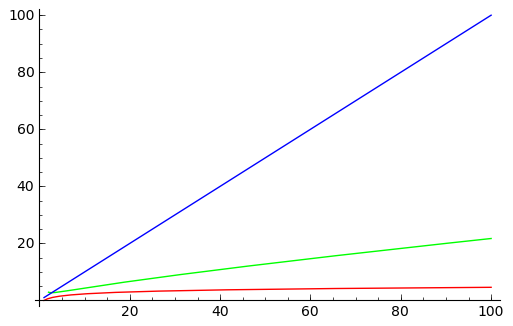
\includegraphics[height=4cm]{figures/xundlnxundxdurchlnx.png}
	\caption{Die Funktionen $x$ (blau), $\ln{x}$ (rot)
                 und $\frac{x}{\ln{x}}$ (grün)}
	\label{xundlnxundxdurchlnx}
        \vskip +15pt
\end{figure}


\subsubsection*{Die Funktion $PI(x) = \frac{x}{\ln{x}}$}
\index{PI(x), $\Pi(x)$}
Die Funktion $\frac{x}{\ln{x}}$ setzt sich also zusammen aus der Funktion $x$ im Zähler und der im Verhältnis dazu sehr langsam wachsenden Funktion $\ln{x}$ im Nenner. Die Anzahl der Primzahlen kleiner oder gleich einer Zahl $x$ ist zwar verhältnismäßig klein im Vergleich zu $x$ selbst. Dennoch ist $\frac{x}{\ln{x}}$ eine wachsende Funktion. Dies wird auch deutlich in Abbildung \ref{xundlnxundxdurchlnx} auf Seite \pageref{xundlnxundxdurchlnx}.


\subsubsection*{Die Anzahl der Primzahlen in verschiedenen Intervallen}
\label{primes:_Appendix_subsubsection_NumberofPrimes-in-intervals}
Abbildung \ref{deltazehnxdurchlnxbis}
% auf Seite \pageref{deltazehnxdurchlnxbis}
veranschaulicht, wie sich die Anzahl der Primzahlen in den Intervallen
$[1, 10^x]$ und $[10^{x-1},10^{x}]$ entwickelt. Um es schneller
berechnen zu können, wird
nicht die exakte Anzahl (wie in den Tabellen in Kapitel \ref{s:primhfk})
benutzt, sondern der Wert der Näherungsfunktion.

Dabei werden pro Zehner-Exponenten zwei Balken gezeichnet:
$\frac{10^{x}}{\ln{10^{x}}}$ im Vergleich zu $\frac{10^{x}}{\ln{10^{x}}}-\frac{10^{x-1}}{\ln{10^{x-1}}}$:
Die linke Grafik für $x$ von $1$ bis $5$, und die rechte für $x$ von $1$ bis $10$, wobei x der Wert des Zehner-Exponenten ist.\\

Die blauen Balken geben an, wieviele Primzahlen es ingesamt bis $10^x$ gibt.
Die roten Balken zeigen, wieviele Primzahlen jeweils im letzten Intervall
$[10^{x-1},10^x]$ hinzukommen.
Dies verdeutlicht, dass die Anzahl der Primzahlen in Intervallen mit höheren
Exponenten immer noch stark steigt.

\begin{figure}[!htb]
	\centering
	\subfloat[ ]{\label{deltazehnxdurchlnxbis5}
                     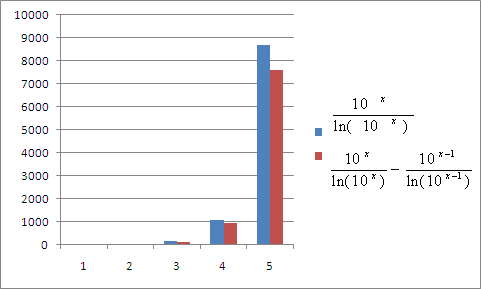
\includegraphics[height=4cm]{figures/deltazehnxdurchlnxbis5.png}}
	\hfill
	\subfloat[ ]{\label{deltazehnxdurchlnxbis10}
                     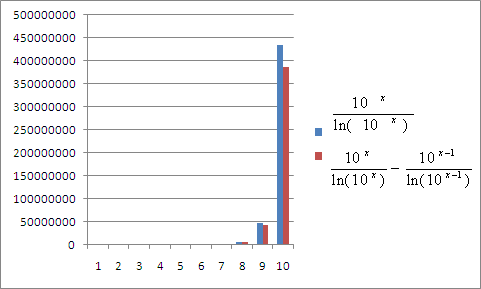
\includegraphics[height=4cm]{figures/deltazehnxdurchlnxbis10.png}}
	\caption{Anzahl der Primzahlen im Intervall $[1, 10^x]$ (blau) und im
         Intervall $[10^{x-1},10^x]$ (rot) (für verschiedene Exponenten $x$)}
	\label{deltazehnxdurchlnxbis}
\end{figure}


Eine Tabelle mit den Anzahlen von Primzahlen in einigen ausgewählten Intervallen
finden Sie in Kapitel \ref{s:primhfk} auf Seite \pageref{s:primhfk}:
Z.B. liegen im Intervall $[1, 10^4]$ 1229 Primzahlen; davon befinden sich im
Intervall $[10^3, 10^4]$ 1229 - 168 = 1061 Primzahlen.

Theorie zum Primzahlsatz und zur Funktion PI(x) steht in Kapitel
\ref{l_Primes_Distrib-of-Primes}.



\begin{sagecode}
\begin{Verbatim}%
[fontsize=\footnotesize]

# Definition der Funktion f(x)=x und Plots für die Definitionsbereiche 0 bis 10^10 und 0 bis 100
sage: def f(x):return x
....:
sage: F=plot(f,(0,10^10))
sage: F.plot()

sage: F2=plot(f,(1,100))
sage: F2.plot()


# Definition der Funktion g(x)=10^x und Plot für den Definitionsbereich 0 bis 10
sage: def g(x): return 10^x
....:
sage: G=plot(g,(0,10))
sage: G.plot()


# Definition der Funktion h(x)=log(x) und Plots für die Definitionsbereiche 1 bis 100 und 1 bis 10^10
sage: def h(x): return log(x)
....:
sage: H=plot(h,(1,100),color="red")
sage: H.plot()

sage: H2=plot(h,(1,10^10),color="red")
sage: H2.plot()


# Definition der Funktion k(x)=x/log(x) und Plot für den Definitionsbereich 2 bis 100
sage: def k(x): return x/log(x)
....:
sage: K=plot(k,(2,100),color="green")
sage: K.plot()


# Plot der Funktionen f, k und h für den Definitionsbereich von 1 bzw. 2 bis 100
sage: F2+K+H


# Generieren der Daten für die Balkencharts ..........................
# Bestimmen der Anzahl der Primzahlen im Intervall [1,10]
sage: pari(10).primepi()-pari(1).primepi()
4

# Bestimmen der Anzahl der Primzahlen im Intervall [10^3,10^4]
sage: pari(10**4).primepi()-pari(10**3).primepi()
1061

# Bestimmen der Anzahl der Primzahlen im Intervall [10^8,10^9]
sage: pari(10**9).primepi()-pari(10**8).primepi()
45086079

# (ab 10^10: OverflowError: long int too large to convert)

\end{Verbatim}
\caption{Erzeugen der Graphen zu den drei Funktionen x, log(x) und x/log(x)}
\end{sagecode}




% ---------------------------------------------------------------------------
% ---------------------------------------------------------------------------
\clearpage
\newpage
\hypertarget{primes:_Appendix_Sage-Samples}{}
\section{Anhang: Beispiele mit SageMath}
% \section*{Appendix A: Beispiele mit SageMath}
% \addcontentsline{toc}{section}{Appendix A: Beispiele mit SageMath}
\label{primes:_Appendix_Sage-Samples}
\index{SageMath!Programmbeispiele}
\index{SageMath}

 Der folgende Abschnitt enthält SageMath Source-Code zu den Inhalten aus
Kapitel~\ref{Chapter_Primes} (\glqq \nameref{Chapter_Primes}\grqq).


% ---------------------------------------------------------------------------
% \newpage
\subsection{Einfache Funktionen zu Primzahlen mit SageMath}
\index{SageMath}

In diesem Teil des Anhangs finden Sie den Quellcode für SageMath, mit dem man
einige einfache Berechnungen zu Primzahlen durchführen kann.%
\footnote{Siehe die SageMath-Dokumentation über Elementare Zahlentheorie
   \url{http://doc.sagemath.org/html/en/constructions/number_theory.html}.}

\begin{sagecode}
\begin{Verbatim}%
[fontsize=\footnotesize]

# Primzahlen (allgemeine Befehle)
# Die Menge der Primzahlen
sage: P=Primes(); P
Set of all prime numbers: 2, 3, 5, 7, ...

# Gibt die nächste Primzahl aus
sage: next_prime(5)
7

# Gibt die Anzahl der Primzahlen <=x aus
sage: pari(10).primepi()
4

# Gibt die ersten x Primzahlen aus
sage: primes_first_n(5)
[2, 3, 5, 7, 11]

# Gibt die Primzahlen in einem Interval aus
sage: list(primes(1,10))
[2, 3, 5, 7]

\end{Verbatim}
\caption{Einige einfache Funktionen zu Primzahlen}
\end{sagecode}



% ---------------------------------------------------------------------------
\newpage
\subsection{Primalitäts-Check der von einer quadratischen Funktion erzeugten Zahlen}
\index{SageMath}

In diesem Anhang finden Sie den Quellcode für SageMath, mit dem man
z.B.\ prüfen kann, ob die von der Funktion $f(n) = n^2 - 9n + 61$
erzeugten Zahlen prim sind.
Der Quellcode definiert eine Funktion namens \verb!quadratic_prime_formula()!,
die die folgenden drei Argumente hat:
\begin{itemize}
\item \verb!start! --- Ein natürliche Zahl, die die Untergrenze der Folge
  $\texttt{start}, \texttt{start} + 1,
  \texttt{start} + 2, \dots, \texttt{end} - 1, \texttt{end}$ darstellt.

\item \verb!end! --- Ein natürliche Zahl, die die Obergrenze der Folge
  $\texttt{start}, \texttt{start} + 1,
  \texttt{start} + 2, \dots, \texttt{end} - 1, \texttt{end}$ darstellt.

\item \verb!verbose! --- (Standardwert: \verb!True!) Ein Schalter, der festlegt,
  ob für jede erzeugte Einzelzahl $f(n)$ eine Ausgabe zur Primalität erfolgen soll.
\end{itemize}

 Eine sinnvolle Änderung dieses Codes besteht darin, eine andere Funktion anzugeben,
deren Funktionswerte auf Primalität geprüft werden sollen.


\begin{sagecode}
\begin{Verbatim}%
[fontsize=\footnotesize]
def quadratic_prime_formula(start, end, verbose=True):
    print "N -- N^2 - 9*N + 61"
    P = 0 # the number of primes between start and end
    for n in xrange(start, end + 1):
        X = n^2 - 9*n + 61
        if is_prime(X):
            P += 1
            if verbose:
                 print str(n) + " -- " + str(X) + " is prime"
        else:
            if verbose:
                 print str(n) + " -- " + str(X) + " is NOT prime"
    print "Number of primes: " + str(P)
    print "Percentage of primes: " + str(float((P * 100) / (end - start + 1)))
\end{Verbatim}
\caption{Testen der Primalität von Funktionswerten, erzeugt von einer quadratischen Funktion}
\end{sagecode}

\vspace{12pt}
Mit dem folgenden Funktionsaufruf berechnen wir die Werte von $f(n) = n^2 - 9n + 61$
für $n = 0, 1, 2, \dots, 50$ und verifizieren die Primalität der erzeugten Funktionswerte:

\begin{Verbatim}%
[fontsize=\footnotesize]
sage: quadratic_prime_formula(0, 50)
 N -- N^2 - 9*N + 61
0 -- 61 is prime
1 -- 53 is prime
2 -- 47 is prime
3 -- 43 is prime
4 -- 41 is prime
5 -- 41 is prime
6 -- 43 is prime
7 -- 47 is prime
8 -- 53 is prime
9 -- 61 is prime
10 -- 71 is prime
11 -- 83 is prime
12 -- 97 is prime
13 -- 113 is prime
14 -- 131 is prime
15 -- 151 is prime
16 -- 173 is prime
17 -- 197 is prime
18 -- 223 is prime
19 -- 251 is prime
20 -- 281 is prime
21 -- 313 is prime
22 -- 347 is prime
23 -- 383 is prime
24 -- 421 is prime
25 -- 461 is prime
26 -- 503 is prime
27 -- 547 is prime
28 -- 593 is prime
29 -- 641 is prime
30 -- 691 is prime
31 -- 743 is prime
32 -- 797 is prime
33 -- 853 is prime
34 -- 911 is prime
35 -- 971 is prime
36 -- 1033 is prime
37 -- 1097 is prime
38 -- 1163 is prime
39 -- 1231 is prime
40 -- 1301 is prime
41 -- 1373 is prime
42 -- 1447 is prime
43 -- 1523 is prime
44 -- 1601 is prime
45 -- 1681 is NOT prime
46 -- 1763 is NOT prime
47 -- 1847 is prime
48 -- 1933 is prime
49 -- 2021 is NOT prime
50 -- 2111 is prime
Number of primes: 48
Percentage of primes: 94.1176470588
\end{Verbatim}

 Die Statistik in den letzten beiden Zeilen der Ausgabe zeigt, dass
$f(n)$ 48 Primzahlen erzeugt für $0 \leq n \leq 50$, was ca. 94\% der von
$f(n)$ erzeugten Werte darstellt.\\

Bei längeren Sequenzen ist die Einzelausgabe der erzeugten Zahl und ihrer Primalität
ziemlich unpraktisch. Deshalb wird in der folgenden SageMath-Session nur die Statistik am
Ende ausgegeben (indem man den Verbose-Parameter auf False setzt): die Gesamtzahl und
der prozentuale Anteil der Primzahlen, die von
$f(n)$ im Bereich $0 \leq n \leq 1000$ erzeugt wurde.

\begin{Verbatim}%
[fontsize=\footnotesize]
sage: quadratic_prime_formula(0, 1000, verbose=False)
N -- N^2 - 9*N + 61
Number of primes: 584
Percentage of primes: 58.3416583417
\end{Verbatim}





%------------------------------------------------------------------------------

\printbibliography[%
	heading=subbibintoc,
	title={Literatur zu Kapitel \thechapter},
	segment=\therefsegment,
]

 Alle Links wurden am 11.07.2016 überprüft.


% --------------------------------------------------------------------------
\newpage
\chapter*{Web-Links}\addcontentsline{toc}{section}{Web-Links}

\begin{enumerate}
   \item GIMPS (Great Internet Mersenne Prime Search)
      \index{Mersenne!Mersenne-Primzahl} \\
         www.mersenne.org ist die Homepage des GIMPS-Projekts, \index{GIMPS} \\
      \url{http://www.mersenne.org/primes/}

\item Die Proth Search Page mit dem Windows-Programm von Yves Gallot \\
      \url{http://primes.utm.edu/programs/gallot/index.html}

\item Verallgemeinerte Fermat-Primzahlen-Suche \\
      \url{http://primes.utm.edu/top20/page.php?id=12}

\item Verteilte Suche nach Teilern von Fermatzahlen \\
      \url{http://www.fermatsearch.org/}

%\item An der Universität von Tennessee findet man umfangreiche
%      Forschungsergebnisse über Primzahlen. \\
\item Die Universität von Tennessee hostet umfangreiche
      Forschungsergebnisse über Primzahlen. \\
      \url{http://www.utm.edu/}

\item Den besten Überblick zu Primzahlen (weil sehr aktuell und vollständig)
      bieten m.E.  ~\glqq The Prime Pages\grqq~ von Professor Chris Caldwell.
      \index{Caldwell, Chris} \\
      \url{http://primes.utm.edu/}

\item Beschreibungen u.a. zu Primzahltests\\
      \url{http://primes.utm.edu/mersenne/index.html}\\
      \url{http://primes.utm.edu/prove/index.html}

\item Ausgabe der $n$-ten Primzahl P(n)\\
      \url{https://primes.utm.edu/notes/by_year.html}\\
      \url{https://primes.utm.edu/nthprime/}

\item Der Supercomputerhersteller SGI Cray Research beschäftigte nicht
      nur hervorragende Mathematiker, sondern benutzte die Primzahltests
      auch als Benchmarks für seine Maschinen.\\
      \url{http://www.isthe.com/chongo/tech/math/prime/prime_press.html}

\item Das Cunningham-Projekt\index{Cunningham-Projekt}\\
      \url{http://www.cerias.purdue.edu/homes/ssw/cun/}

\item EFF Cooperative Computing Awards\\
	\url{https://www.eff.org/awards/coop}

\item Goldbach conjecture verification project von Tomás Oliveira e Silva,
      \index{Goldbach-Projekt}\\
      \url{http://sweet.ua.pt/tos/goldbach.html}

\item Kurt Gödel\\
	\url{https://www.mathematik.ch/mathematiker/goedel.php}

% Info: http://www.mathematik.ch/mathematiker/Goldbachsche_Vermutung.php
% tot: \item \url{http://www.informatik.uni-giessen.de/staff/richstein/de/Goldbach.html}
% tot: \item \url{http://www.mscs.dal.ca/~dilcher/golbach/index.html}
% tot:       \url{http://www.mscs.dal.ca/~joerg/res/g-en.html}

% tot: \item \url{http://www.informatik.tu-darmstadt.de/TI/LiDIA/}

% tot: \item \url{http://www.math.Princeton.EDU/~arbooker/nthprime.html}
	% {\tt http://www.math.Princeton.EDU/\~{}arbooker/nthprime.html}
	% Nun bei http://www.maths.bris.ac.uk/~maarb/public/papers/
	% (Reader of Pure Mathematics) andrew.booker@bristol.ac.uk

\end{enumerate}

 Alle Links wurden am 06.08.2018 überprüft.



\vskip +10 pt
% --------------------------------------------------------------------------(5\cdot2^7 - 1)(5^2\cdot2^14 + 1)
\section*{Dank} \addcontentsline{toc}{section}{Dank}
Für das sehr konstruktive Korrekturlesen der ersten Versionen
dieses Artikels: Hr. Henrik Koy und Hr. Roger Oyono.




\end{refsegment}
% Local Variables:
% TeX-master: "../script-de.tex"
% End:(5\cdot2^7 - 1)(5^2\cdot2^14 + 1)(5\cdot2^7 - 1)(5^2\cdot2^14 + 1)
